%% ============================================================
%%  From Retrospective Benchmarking to Anticipatory Policy: A Data Driven Framework for Governance Indexing and
%%  Forecasting Using the Viet Nam Provincial Governance and Public Administration Performance Index (PAPI)
%%
%%  Author    : Ngoc Kim Son Hoang
%%  Affiliation: Faculty of Development Economics,
%%               VNU University of Economics and Business,
%%               Vietnam National University, Hanoi 10000, Vietnam
%%  Email     : 23050613@vnu.edu.vn
%%
%%  Compile   : xelatex main.tex (twice for cross-references)
%%              biber main
%%              xelatex main.tex (twice again)
%% ============================================================

\documentclass[12pt,a4paper]{article}

% ---------- Encoding & Fonts ----------
\usepackage{fontspec}
\setmainfont[
  Path=./font/,
  Extension=.ttf,
  UprightFont=CharisSIL-Regular,
  ItalicFont=CharisSIL-Italic,
  BoldFont=CharisSIL-Bold,
  BoldItalicFont=CharisSIL-BoldItalic
]{CharisSIL-Regular}
\usepackage[%
  stretch=25,%
  shrink=25,%
  step=1%
]{microtype}         % Improved justification with character protrusion and expansion

% ---------- Page Layout ----------
\usepackage[
  top=25mm, bottom=20mm,
  left=20mm, right=20mm,
  headheight=15pt
]{geometry}

% ---------- Hyphenation & Line Breaking ----------
\hyphenpenalty=50           % Encourage hyphenation for better line breaking
\exhyphenpenalty=50         % Allow hyphenation after explicit hyphens
\doublehyphendemerits=6500  % Discourage consecutive hyphenated lines
\widowpenalty=5000          % Strong penalty for widow lines
\clubpenalty=5000           % Strong penalty for orphan lines
\raggedbottom               % Allow flexible bottom margins

% ---------- Line Spacing ----------
\usepackage{setspace}
\onehalfspacing

% ---------- Mathematics ----------
\usepackage{amsmath}
\usepackage{amssymb}
\usepackage{amsthm}
\usepackage{bm}                % bold math symbols
\usepackage{mathtools}
\usepackage{siunitx}
\sisetup{
  table-alignment=right,
  table-number-alignment=right,
  separate-uncertainty=true,
  multi-part-units=single,
  group-minimum-digits=4
}

% ---------- Figures & Tables ----------
\usepackage{graphicx}
\usepackage{booktabs}
\usepackage{tabularx}
\usepackage{multirow}
\usepackage{array}
\usepackage{longtable}
\usepackage{float}
\usepackage{caption}
\usepackage{subcaption}
\captionsetup{
  font=small,
  labelfont=bf,
  skip=6pt,
  justification=justified,
  singlelinecheck=false
}

% ---------- Table Configuration ----------
\renewcommand{\arraystretch}{1.1}  % Slightly increase vertical padding in tables

% ---------- Lists ----------
\usepackage{enumitem}
\setlist{itemsep=2pt, topsep=4pt}

% ---------- Colors ----------
\usepackage[dvipsnames]{xcolor}
\definecolor{linkblue}{RGB}{0,70,140}

% ---------- Hyperlinks ----------
\usepackage[
  colorlinks=true,
  linkcolor=black,
  citecolor=black,
  urlcolor=black,
  bookmarksopen=true,
  pdfauthor={Ngoc Kim Son Hoang},
  pdftitle={From Retrospective Benchmarking to Anticipatory Policy: A Data Driven Framework for Governance Indexing and Forecasting Using the Viet Nam Provincial Governance and Public Administration Performance Index (PAPI)}
]{hyperref}

% ---------- Headers & Footers ----------
\usepackage{fancyhdr}
\pagestyle{fancy}
\fancyhf{}
\fancyhead[L]{\small\textit{From Benchmarking to Anticipatory Policy: A Data-Driven Governance Framework}}
\fancyhead[R]{\small\textit{Hoang, N.K.S.}}
\fancyfoot[C]{\thepage}
\renewcommand{\headrulewidth}{0.4pt}

% ---------- Bibliography ----------
\usepackage[style=apa, backend=biber, natbib=true]{biblatex}
\addbibresource{main.bib}


% ---------- Miscellaneous ----------
\usepackage{xspace}
\usepackage{lipsum}   % placeholder text
\usepackage{url}
\urlstyle{same}
\usepackage{ragged2e} % For justify environment

% Prevent floats from breaking paragraphs
\usepackage{placeins}

% ---------- Custom Commands ----------
\newcommand{\PAPI}{\textsc{papi}\xspace}
\newcommand{\MCDM}{\textsc{mcdm}\xspace}
\newcommand{\MICE}{\textsc{mice}\xspace}
\newcommand{\CRITIC}{\textsc{critic}\xspace}
\newcommand{\TOPSIS}{\textsc{topsis}\xspace}
\newcommand{\VIKOR}{\textsc{vikor}\xspace}
\newcommand{\COPRAS}{\textsc{copras}\xspace}
\newcommand{\EDAS}{\textsc{edas}\xspace}
\newcommand{\PROMETHEE}{\textsc{promethee}\xspace}
\newcommand{\SAW}{\textsc{saw}\xspace}
\newcommand{\OOF}{\textsc{oof}\xspace}
\newcommand{\CI}{\textsc{ci}\xspace}
\newcommand{\ie}{\textit{i.e.,}\xspace}
\newcommand{\eg}{\textit{e.g.,}\xspace}

\newtheorem{definition}{Definition}
\newtheorem{proposition}{Proposition}

% =============================================================
%  TITLE PAGE
% =============================================================

\begin{document}

\begin{titlepage}
  \centering
  \vspace*{-2cm}

  {\LARGE\bfseries
    From Retrospective Benchmarking to Anticipatory Policy: A Data Driven Framework for Governance Indexing and Forecasting Using the Viet Nam Provincial Governance and Public Administration Performance Index (PAPI)
  \par}

  \vspace{1cm}

  {\large Hoang Ngoc Kim Son}

  \vspace{0.5cm}

  {\large \textit{Supervised by:} Assoc. Prof. Luu Quoc Dat}
  
  \vspace{0.5cm}

  {\normalsize
    Faculty of Development Economics,\\
    VNU University of Economics and Business,\\
    Vietnam National University, Hanoi 10000, Vietnam\\[4pt]
    Correspondence:  23050613@vnu.edu.vn
  }
  
  \vspace{1.0cm}
  
  {\small March 19, 2026}

  \vspace{0.5cm}

  \hrule

  \vspace{1cm}

  {\large\textbf{Abstract}}

  {\footnotesize
  \begin{justify}
  Governance assessments in developing economies typically rely on equal-weighting and single-method ranking, precluding temporal forecasting and proactive policymaking. Addressing this, this study develops a three-tier framework for subnational governance indexing and probabilistic forecasting, validated on Vietnam's Provincial Governance and Public Administration Performance Index (\textsc{papi}) dataset (2011--2024). The framework integrates: (i) a hierarchical \textsc{critic} weighting model capturing multidimensional information; (ii) a multi-method consensus ranking of five distinct decision algorithms (\textsc{topsis}, \textsc{vikor}, \textsc{promethee~ii}, \textsc{copras}, and \textsc{edas}); and (iii) a stacked ensemble forecasting pipeline combining ten diverse machine learning models. The consensus ranking yields high inter-algorithm concordance (mean $\bar{\rho} = 0.96$), while the stacked ensemble achieves a Mean Absolute Scaled Error of 0.6411, outperforming the best individual baseline by 14.12\%. Projections for 2025 identify 29 provinces at risk of governance contraction, with severe declines (exceeding 40\%) localized in corruption control and digital accessibility. These empirical insights support a proposed Tiered Governance Compact for targeted policy interventions. This work provides a transferable, open-source pipeline to transition global institutional assessment from retrospective benchmarking to anticipatory policymaking.
  \end{justify}
  }

  \vspace{0.5cm}

  \noindent\textbf{Keywords:} Ensemble Machine Learning; Governance Assessment; \textsc{mcdm}; \textsc{papi}; Probabilistic Forecasting; Provincial Governance; Vietnam

  \vspace{0.5cm}
\end{titlepage}

\clearpage
\tableofcontents
\clearpage

% =============================================================
\section{Introduction}
\label{sec:introduction}

% ============================================================
% MOVE 1: ESTABLISHING A TERRITORY (CONTEXT)
% ============================================================

The empirical assessment of sub-national governance capacity has emerged as a critical frontier in development economics and institutional research. Effective governance, operationalized through transparency, accountability, administrative efficiency, and service delivery quality, constitutes a fundamental determinant of economic growth and citizen welfare across developing economies \citep{Acemoglu2012, Kaufmann2011}. In Vietnam's transition to a market-oriented system, institutional reforms at provincial levels remain uneven across 63 administrative divisions \citep{PAPI2024}.

Over the past fifteen years, multiple governance assessment frameworks have been institutionalized within Vietnam to benchmark provincial performance and catalyze administrative reform. The Provincial Governance and Public Administration Performance Index (\PAPI), administered jointly by CECODES, the Vietnam Fatherland Front Research and Training Committee, and the United Nations Development Programme, has established itself as the preeminent system for measuring citizen-perceived governance quality across eight hierarchically-organized dimensions, including civic participation, transparency, accountability, anti-corruption efficacy, administrative procedural efficiency, public service delivery quality, environmental governance, and e-governance accessibility \citep{PAPI2024}. Parallel frameworks interrogate complementary dimensions: the Satisfaction Index of Public Administrative Services (SIPAS) focuses on citizen satisfaction with bureaucratic transactions; the Provincial Competitiveness Index (PCI) combines governance metrics with economic and business-environment indicators; the Digital Transformation Index (DTI) assesses technological adoption and digital service maturity; and the Public Administration Reform Index (PAR Index) tracks incremental progress in administrative modernization. Collectively, these indices constitute a rich empirical substrate for comparative provincial governance assessment, yet their methodological foundations remain fragmented, frequently relying on ad hoc aggregation choices rather than principled, data-driven approaches \citep{Greco2016}.

The dominant methodological in governance indexing practice, both in Vietnam and globally, has gravitated toward composite index construction via equal weighting of constituent indicators. This paradigm assumes that all dimensions contribute equally to the composite governance construct, assigning each indicator a symmetric $1/n$ normalizing weight. While equal weighting offers transparent communicability and computational simplicity, it confronts a critical limitation: equal weighting discards two vital sources of empirical information embedded in the data itself. First, indicators exhibit heterogeneous \emph{discriminatory power}, or contrast intensity, across provinces. An administrative procedure indicator that yields identical scores across all 63 provinces carries zero ranking information, yet under equal weighting receives the same axiological weight as a corruption perception indicator that substantially differentiates provinces. Second, indicators exhibit heterogeneous \emph{redundancy}, or information overlap. When multiple indicators measuring related aspects of governance (e.g., access-to-information versus transparency-of-budget-execution) correlate strongly, equal weighting implies that correlated information is double-counted, inflating its influence in the final composite ranking \citep{Diakoulaki1995, Greco2016}.

Beyond weighting methodology, existing Vietnamese governance indices have adopted singular ranking aggregation methods. The \PAPI composite, for instance, employs simple additive aggregation of normalized component scores after equal weighting. The PCI relies on principal component analysis for dimension reduction, followed by ad hoc element weighting. This reliance on a single aggregation paradigm introduces a fundamental vulnerability: the methodological idiosyncrasy problem. A central theorem in multi-criteria decision analysis establishes that no single aggregation function satisfies all desirable axiomatic properties simultaneously \citep{Arrow1951}. Consequently, rankings derived from any single method risk instability when the underlying preference model is altered marginally.

% ============================================================
% MOVE 2: ESTABLISHING A NICHE (IDENTIFYING THE GAP)
% ============================================================

Despite the maturity attained by Vietnam's governance indices over nearly 14 years of annual measurement (2011--2024), three methodological gaps remain insufficiently addressed in extant applied research and policy practice.

The first gap concerns the absence of data-driven weighting schemes validated against temporal stability and robustness criteria. While equal weighting is often adopted as a convenient default rather than a reflection of true equal importance \citep{Seth2018}, recent literature increasingly advocates for objective weighting to capture actual data variance and structural correlations \citep{Greco2018, Becker2017}. Objective methods have been shown to significantly enhance discriminatory power and reduce arbitrary rank distortions in composite indices, though their robustness depends on proper methodological constraints \citep{Liborio2024}. However, current Vietnamese indices continue to employ either equal weighting, which is canonical yet informationally wasteful, or subjective expert weighting, which is transparent in rationale but vulnerable to expert bias and unstable across different panels. No published study systematically applies objective weighting methods, such as the Criteria Importance Through Intercriteria Correlation (CRITIC) method, to the hierarchical structure of the \PAPI or its peer indices, nor does extant literature validate whether estimated weights exhibit temporal stability across the full measurement window (2011--2024) or remain robust to methodological perturbations. This gap is non-trivial: if governance priorities shift substantially over 14 years, a single unified weight vector may conceal important structural breaks; conversely, if weights prove unstable, confidence in the underlying governance assessment methodology itself is undermined. Formal temporal validation and sensitivity analysis remain conspicuously absent from the governance indexing literature on Vietnam.

The second gap involves the absence of multi-methodological ranking frameworks that achieve robustness across diverse MCDM algorithms. The architectural assumption implicit in single-method ranking, that a particular mathematical formalism (distance minimization, outranking logic, or proportional aggregation) correctly encodes the governance assessment problem, lacks empirical validation. No published study applies a multi-method ensemble of MCDM algorithms to Vietnamese governance data, nor does extant research characterize the sensitivity of provincial rankings to methodological variation. This omission is significant because practitioners and policymakers require confidence that provincial governance orderings reflect genuine performance differentiation, not ephemeral artifacts of mathematical choice. A ranking framework incorporating multiple methods would substantially elevate methodological credibility and policy robustness.

The third gap stems from the disconnection between static MCDM ranking assessment and dynamic temporal forecasting of future governance trajectories. Existing governance indices are inherently retrospective in nature, ranking provinces based on observed data from a single calendar year or multi-year average, without explicitly projecting likely governance evolution. However, predictive analytics have begun to shift public policy frameworks globally from retrospective benchmarking toward anticipatory governance and scenario simulation \citep{Maffei2020, Williamson2016}. By leveraging machine learning, policymakers can transition toward proactive intervention and forward-looking institutional design \citep{Athey2017}. For forward-looking governance planning and resource allocation in Vietnam, policymakers require not only current rankings but also probabilistic forecasts of future performance. Machine learning ensemble forecasting, which combines diverse base learners with metalearned combination weights, constitutes a methodologically mature framework for this temporal prediction. Yet no study integrates hierarchical MCDM, temporal weighting validation, and ensemble machine learning forecasting into a unified governance assessment architecture. The absence of this integration means that governance assessment remains siloed from the powerful arsenal of time-series and ensemble learning methodologies that have transformed demand forecasting, economic nowcasting, and other high-stakes prediction domains \citep{Hastie2009, Wolpert1992}.

% ============================================================
% MOVE 3: OCCUPYING THE NICHE (SOLUTION & CONTRIBUTION)
% ============================================================

To address these three gaps simultaneously, this study develops and validates a comprehensive hybrid framework for governance assessment applied to PAPI data spanning 14 years and 63 provinces. The framework synthesizes three complementary innovations: hierarchical CRITIC weighting with temporal stability validation; multi-methodological MCDM ranking transcending single-method idiosyncrasy; and ensemble machine learning forecasting with calibrated uncertainty quantification.

The first innovation involves hierarchical CRITIC weighting with temporal stability validation. The methodological extension applies the classical CRITIC method, which derives criterion weights from data heterogeneity (variance) and inter-criterion independence (correlation), to a novel two-level hierarchical architecture tailored to the multi-tier structure of the PAPI dataset. Level 1 applies \CRITIC independently within each of the 8 governance criteria, computing data-driven weights for the 29 constituent sub-criteria while respecting hierarchy and preventing over-weighting of sub-criteria in weak-signal criteria. Level 2 applies \CRITIC across the 8 criterion-level composite scores, reflecting both within-criterion redundancy mitigation (Level 1) and inter-criterion information assessment. Critically, multi-window temporal stability analysis is conducted using overlapping 5-year windows, Spearman's rank correlation, Kendall's omnibus concordance coefficient $W$, and per-criterion coefficient-of-variation metrics. This analysis empirically establishes whether governance prioritization (operationalized through the weight vector) exhibits sufficient temporal consistency across the 14-year span to justify deployment as a unified parameter, or whether time-variant weighting would be warranted. Additionally, three-tier Monte Carlo perturbation sensitivity analysis (conservative ±5\%, moderate ±15\%, aggressive ±50\%) quantifies ranking robustness to weight specification uncertainty, addressing a critical but under-examined aspect of indexing methodology.

The second innovation establishes a multi-methodological MCDM ranking framework. Rather than relying on a single ranking algorithm, the framework employs an ensemble of five distinct MCDM methods representing three orthogonal aggregation paradigms: (i) distance-based (TOPSIS), (ii) outranking (VIKOR, PROMETHEE), and (iii) proportional assessment (COPRAS, EDAS). For each method and each year (2011--2024), independent provincial rankings are generated. Rank-order correlations and agreement indices (Spearman's $\rho$, Kendall's tau-b) characterize inter-method concordance, identifying methodological consensus regions and divergence zones. Final provincial rankings are derived via weighted aggregation of method-specific rankings.

The third innovation concerns integration with ensemble machine learning forecasting. The validated weighting scheme and multi-method ranking framework are integrated into an ensemble forecasting pipeline that projects likely governance trajectories (2025). A heterogeneous set of ten base learners, spanning classical statistical models (Naive, AutoARIMA, AutoETS), tabular machine learning (RecursiveTabular, DirectTabular), deep learning architectures (PatchTST, TemporalFusionTransformer, DeepAR), a foundation model (Chronos), and an optimized classical model (DynamicOptimizedTheta), is trained on the panel dataset using modular feature engineering. Stacking is operationalized using AutoGluon's \texttt{WeightedEnsemble} framework, wherein a second-level meta-learner optimizes combination weights on out-of-fold predictions. Out-of-sample predictive performance is evaluated using Mean Absolute Scaled Error (MASE) across multiple validation windows, while probabilistic forecasting is enabled through quantile regression to construct 80\% prediction intervals that quantify forecast uncertainty.

The full framework is implemented in a reproducible, modular Python software architecture, enabling practitioners and policymakers to apply the approach to Vietnam's governance indices or parallel assessment frameworks. A rigorous comparative validation demonstrates that the hierarchical CRITIC-weighted, multi-method MCDM approach yields rankings that are temporally stable, methodologically robust, and substantially concordant across diverse aggregation algorithms, representing improvements over existing practice.

The paper proceeds as follows. Section 2 describes the data structure, presents the hierarchical CRITIC weighting procedure with temporal stability and sensitivity analysis, specifies the multi-method MCDM framework and ensemble machine learning forecasting architecture. Section 3 presents empirical results on temporal weight evolution, divergence across MCDM methods, and ensemble forecasting projects governance trajectories through 2025. Section 4 synthesizes findings, contextualizes contributions, discusses policy implications, and identifies future research directions.


% =============================================================
\section{Methods and Data}
\label{sec:methods}
% =============================================================

\subsection{Data Description}
\label{subsec:data}

The Provincial Governance and Public Administration Performance Index (\PAPI) is Viet Nam's premier citizen-centric diagnostic tool, designed to assess the performance of subnational authorities in governance, public administration, and public service delivery. Jointly initiated and administered since 2009 (achieving nationwide coverage of all 63 provinces in 2011) by the Centre for Community Support and Development Studies (CECODES), the Vietnam Fatherland Front Research and Training Committee (VFF-CRT), and the United Nations Development Programme (UNDP), \PAPI serves as a critical bridge between citizen feedback and policy reform \citep{PAPI2024}. Unlike business-oriented metrics like the Provincial Competitiveness Index (PCI), which capture the perceptions of private firms, \PAPI focuses exclusively on the lived experiences and direct encounters of ordinary citizens with local administration. Utilizing a rigorous, multi-stage stratified random sampling design, the index draws on annual face-to-face interviews with a nationally representative sample of approximately 14,000 to 16,000 citizens, ensuring the representation of diverse demographic, ethnic, and geographic groups. By systematically aggregating bottom-up feedback, \PAPI provides international and domestic researchers with a robust dataset to analyze institutional variation, public policy efficacy, and administrative modernization across Viet Nam's subnational jurisdictions.

% ================================================================
% Section 2.1: PAPI Dataset as Multi-Level Longitudinal Structure
% ================================================================

The PAPI dataset represents a multi-level longitudinal panel of provincial governance indicators spanning 14 annual waves (2011\--2024) with hierarchical structuring: temporal dimension (survey year $t$), spatial dimension (province $i$), and conceptual dimension (governance criteria and sub-criteria).

\subsubsection{Panel Structure and Dimensionality}

The dataset comprises observations of $N = 63$ Vietnamese provinces and centrally administered municipalities (hereafter provinces) measured annually across $T = 14$ survey waves. The underlying constructs are measured through $K = 8$ criteria (denoted $C_k$ for $k = 1, \ldots, 8$), each composed of multiple sub-criteria (denoted $\text{SC}_{jk}$ for $j = 1, \ldots, n_k$). In total, there are $p = 29$ sub-criteria distributed across all criteria.

The data define a balanced panel in spatial ($N = 63$ provinces) and temporal ($T = 14$ years) dimensions, yielding a theoretical maximum of $M = N \times T = 882$ province-year observations. Each observation indexed by $(i, t)$ contains measurements of all $p = 29$ sub-criteria (subject to structural missingness, discussed in Section~\ref{subsec:missing}).

Data collection occurs annually during each survey wave. The survey is administered by Centre for Community Support \& Development Studies (CECODES), the Vietnam Fatherland Front Research and Training Committee (VFF-CRT), and the United Nations Development Programme (UNDP) in collaboration with provincial statistical offices. Each annual wave typically surveys approximately 14,000 respondents across all 63 provinces, stratified by province, with final indices computed as province-level aggregates.

Survey data are collected and published on an annual calendar. The 14 waves span 2011--2024 inclusive:

$$\mathcal{T} = \{2011, 2012, \ldots, 2024\}$$

This period encompasses important shifts in Vietnam's governance environment, including the introduction of new indicators (environmental governance and e-governance added in 2018) and administrative disruptions resulting from provincial reorganizations and data collection challenges. The 14-year span provides sufficient temporal variation for forecasting model training.

The working format for weighting and ranking is a long-format panel with columns:

$$\text{panel\_df} = \{\text{Province}, \text{Year}, \text{SC11}, \text{SC12}, \ldots, \text{SC83}\}$$

Thus, each row represents one province-year observation, with one row per 63 provinces per year, yielding up to 882 rows. Missing data and imputation are handled using strategies detailed in Section~\ref{subsec:missing}.

\subsubsection{Measurement Framework and Indicator Definitions}

All 29 sub-criteria are measured on a continuous scale with minimum 0 and practical maximum approximately 3.33 (reflecting the underlying survey instrument's design). Crucially, all sub-criteria are benefit-type indicators, meaning that higher values indicate stronger governance performance in the respective dimension. This uniform directionality has important implications for MCDM normalization and aggregation (discussed in Sections~\ref{subsec:critic} and~\ref{subsec:mcdm}).

The hierarchical composition of criteria and sub-criteria is presented in Table~\ref{tab:hierarchy}. Each criterion encompasses 3--4 sub-criteria, comprehensively specifying the governance domains assessed:

\newcolumntype{C}[1]{>{\centering\arraybackslash}m{#1}}

\begin{table}[!ht]
\centering
\caption{Comprehensive hierarchical structure of PAPI criteria and sub-criteria with measurement framework}
\label{tab:hierarchy}
\small
\begin{tabular}{c >{\centering\arraybackslash}m{3.6cm} c l}
\toprule
\textbf{Criterion} & \textbf{Criterion Name} & \textbf{Sub-Criterion} & \multicolumn{1}{c}{\textbf{Sub-Criterion Name}} \\
\midrule
\multirow{4}{*}{$C_1$} & \multirow{4}{3.6cm}{\centering Civic Participation} & SC11 & Civic Knowledge \\
 & & SC12 & Opportunities for Participation in Elections \\
 & & SC13 & Quality of Village Head Elections \\
 & & SC14 & Voluntary Contributions \\
\midrule
\multirow{4}{*}{$C_2$} & \multirow{4}{3.6cm}{\centering Transparency of Local Decision-Making} & SC21 & Access to Information \\
 & & SC22 & Poverty List Transparency \\
 & & SC23 & Communal Budget Transparency \\
 & & SC24 & Transparent Land-Use Plan/Price Frames \\
\midrule
\multirow{3}{*}{$C_3$} & \multirow{3}{3.6cm}{\centering Vertical Accountability} & SC31 & Interactions With Local Authorities \\
 & & SC32 & Governments Responsive to Citizen Appeals \\
 & & SC33 & Access to Justice Services \\
\midrule
\multirow{4}{*}{$C_4$} & \multirow{4}{3.6cm}{\centering Control of Corruption in Public Sector} & SC41 & Limits on Corruption in Local Governments \\
 & & SC42 & Limits on Corruption in Service Delivery \\
 & & SC43 & Equity in State Employment \\
 & & SC44 & Willingness to Fight Corruption \\
\midrule
\multirow{4}{*}{$C_5$} & \multirow{4}{3.6cm}{\centering Public Administrative Procedures} & SC51 & Certification Procedures \\
 & & SC52 & Construction Permits \\
 & & SC53 & Land Title Procedures \\
 & & SC54 & Personal Procedures \\
\midrule
\multirow{4}{*}{$C_6$} & \multirow{4}{3.6cm}{\centering Public Service Delivery} & SC61 & Public Healthcare \\
 & & SC62 & Primary Education \\
 & & SC63 & Basic Infrastructure \\
 & & SC64 & Law and Order \\
\midrule
\multirow{3}{*}{$C_7$} & \multirow{3}{3.6cm}{\centering Environmental Governance} & SC71 & Environmental Protection \\
 & & SC72 & Quality of Air \\
 & & SC73 & Quality of Water \\
\midrule
\multirow{3}{*}{$C_8$} & \multirow{3}{3.6cm}{\centering E-Governance} & SC81 & Access to E-Government Portals \\
 & & SC82 & Access to the Internet \\
 & & SC83 & E-Responsiveness of Provincial Authorities \\
\bottomrule
\end{tabular}
\end{table}

\FloatBarrier

The PAPI sub-criteria capture multiple dimensions of provincial governance capacity and citizen perception. Criterion $C_1$ (Civic Participation) reflects the extent and inclusiveness of civic engagement in provincial affairs, encompassing electoral participation and consultation mechanisms. Criterion $C_2$ (Transparency of Local Decision-Making) assesses the accessibility of provincial government information and transparency of budget execution and policy decisions. Criterion $C_3$ (Vertical Accountability) measures government responsiveness to citizen grievances and access to justice mechanisms for redress. Criterion $C_4$ (Control of Corruption in the Public Sector) captures the perceived effectiveness of anti-corruption measures and equitable treatment in service delivery. Criterion $C_5$ (Public Administrative Procedures) evaluates the efficiency and simplification of administrative procedures and the burden of compliance on businesses and individuals. Criterion $C_6$ (Public Service Delivery) measures the quality and accessibility of province-delivered public services including healthcare, education, infrastructure, and utilities. Criterion $C_7$ (Environmental Governance) reflects environmental protection, sustainability of natural resources, and response to pollution and climate issues. Finally, Criterion $C_8$ (E-Governance) captures the availability of online government services, digital information systems, and internet accessibility.

\subsection{Missing Data Structure and Data Imputation}
\label{subsec:missing}

% ================================================================
% Section 2.2: Missing Data Analysis and Robust Imputation Strategy
% ================================================================

The \PAPI dataset exhibits substantial structural missingness reflecting both design constraints and administrative disruptions. The data comprise a balanced panel of 63 Vietnamese provinces measured across 14 annual survey waves (2011--2024) with 29 governance sub-criteria per province-year observation, yielding a theoretical maximum of 25,578 data cells (63 $\times$ 14 $\times$ 29). Across this domain, 3,687 cells are missing, corresponding to a global missingness rate of 14.41\%. While non-trivial, this missingness follows deterministic and partially predictable patterns that permit principled recovery. Understanding and properly addressing these missing data is essential to prevent bias propagation in the ensemble forecasting phase.

It is imperative to distinguish the analytical scope of the data imputation procedure within this study's bifurcated framework. The reconstructed dataset, generated through the \MICE algorithm, is specifically and exclusively utilized to facilitate the ensemble machine learning forecasting phase, where maximum temporal and cross-sectional continuity is mathematically required for model training and stability. Conversely, the hierarchical \CRITIC weighting and multi-criteria ranking procedures (Section~\ref{subsec:critic} and~\ref{subsec:mcdm}) respect the empirical integrity of the initial dataset. These phases employ an adaptive exclusion mechanism that calculates composite indices based only on observed sub-criteria for each respective province-year observation, thereby ensuring that the resulting performance rankings are grounded in direct citizen experience rather than imputed values.

\subsubsection{Missing Data Characterization and Quantification}

Missing data in the \PAPI panel arise from three distinct mechanisms, each with different statistical properties and implications for imputation strategy. These mechanisms are systematically categorized and quantified in Table~\ref{tab:missing_by_type}, which provides a comprehensive temporal breakdown of missingness across all 14 survey waves. The subsequent analysis characterizes each type's statistical nature and its empirical justification for specific imputation treatment.

\begin{table}[!ht]
\centering
\caption{Missing data inventory by type and year (original dataset)}
\label{tab:missing_by_type}
\small
\begin{tabular}{c c c c c}
\toprule
\textbf{Year} & \textbf{Type 1} & \textbf{Type 2} & \textbf{Type 3} & \textbf{Total} \\
\midrule
2011 & 441 & 0 & 0 & 441 \\
2012 & 441 & 0 & 0 & 441 \\
2013 & 441 & 0 & 0 & 441 \\
2014 & 441 & 44 & 0 & 485 \\
2015 & 441 & 0 & 0 & 441 \\
2016 & 441 & 0 & 0 & 441 \\
2017 & 441 & 0 & 0 & 441 \\
2018 & 63 & 0 & 16 & 79 \\
2019 & 0 & 0 & 0 & 0 \\
2020 & 0 & 0 & 0 & 0 \\
2021 & 63 & 84 & 0 & 147 \\
2022 & 63 & 0 & 29 & 92 \\
2023 & 63 & 56 & 0 & 119 \\
2024 & 63 & 56 & 0 & 119 \\
\midrule
\textbf{Total} & \textbf{3,402} & \textbf{240} & \textbf{45} & \textbf{3,687} \\
\bottomrule
\end{tabular}
\end{table}

\FloatBarrier

Type 1 missing data reflect the deliberate evolution of the governance index itself, arising from the formal introduction of new sub-criteria and discontinuation of existing ones. Environmental Governance sub-criteria (SC71, SC72, SC73) were not measured from 2011--2017, accounting for $3 \times 7 \times 63 = 1,323$ missing cells. E-Governance sub-criteria (SC81, SC82, SC83) similarly were absent during 2011--2017, with SC83 becoming consistently available only from 2019 onward, contributing $3 \times 7 \times 63 = 1,323$ missing cells in the 2011--2017 interval. The Transparency sub-criterion SC24 was absent in 2011--2017 and reintroduced in 2018, accounting for $7 \times 63 = 441$ missing cells. Administrative Procedures sub-criterion (SC52) was entirely discontinued from 2021 onward, creating $4 \times 63 = 252$ missing cells in the terminal four years. Across these indicator-level absences, Type 1 missingness totals 3,402 cells, representing 92.27\% of all missing data. These missings are deterministic and observable: the measurement agencies maintain explicit knowledge of which indicators were not operational in each year. This property makes Type 1 missingness conceptually Missing At Random (MAR) dependent on the observed year, since the absence stems from known governance index design choices rather than data collection failures or outcome-dependent processes.

Type 2 missingness comprises entire province-year observations where all 29 sub-criteria are absent, reflecting administrative disruptions in data collection rather than structural index design. Nine distinct province-year instances are identified, totaling 240 missing cells (excluding overlap with Type 1 classification). In 2014, provinces P15 and P56 exhibit complete data absence. Three provinces (P14, P15, P18) are entirely absent in 2021. In 2023, provinces P14 and P47 lack data; similarly, P17 and P52 are absent in 2024. These gaps reflect documented administrative disruptions in provincial survey administration, provincial-level data collection failures, or data processing errors. Under the assumption that such collection failures depend on observable administrative variables (provincial administrative capacity, data infrastructure maturity) rather than the underlying governance quality being measured, Type 2 missingness is assessed as MAR conditional on administrative covariates. This characterization justifies the use of conditional imputation methods, including predictive models trained on reporting provinces within the given year, or within-province temporal interpolation.

Type 3 missingness comprises isolated cells within otherwise substantially populated province-year observations, primarily reflecting individual questionnaire item non-responses or data entry errors. Type 3 missingness totals 47 cells (1.28\% of total missingness). In 2018, provinces P14 and P56 each lack eight sub-criteria concentrated in the Transparency and Corruption Control dimensions (SC21--SC24 and SC41--SC44). In 2022, province P15 lacks 16 cells spanning participation, transparency, corruption, and administrative procedures, while province P18 lacks 15 cells in similar domains. These localized absences suggest category-specific non-response patterns or data entry anomalies affecting particular sub-criteria clusters, rather than complete survey failure or measurement design changes. Type 3 missingness is assessed as Missing At Random (MAR), under which MICE imputation incorporating relevant auxiliary variables yields unbiased recovery.

Given that sub-criterion SC52 (Construction Permits, within the Public Administrative Procedures dimension) has been discontinued from 2021 onward, the forecasting procedure (Section~\ref{subsec:ensemble_forecasting}) conducts temporal prediction using the current indicator architecture, excluding sub-criterion SC52 from the imputation dataset and correspondingly producing no forecasts for this criterion.

\begin{table}[!ht]
\centering
\caption{Missing data inventory by type and year (imputation dataset, SC52 excluded)}
\label{tab:missing_by_type_imputed}
\small
\begin{tabular}{c c c c c}
\toprule
\textbf{Year} & \textbf{Type 1} & \textbf{Type 2} & \textbf{Type 3} & \textbf{Total} \\
\midrule
2011 & 441 & 0 & 0 & 441 \\
2012 & 441 & 0 & 0 & 441 \\
2013 & 441 & 0 & 0 & 441 \\
2014 & 441 & 42 & 0 & 483 \\
2015 & 441 & 0 & 0 & 441 \\
2016 & 441 & 0 & 0 & 441 \\
2017 & 441 & 0 & 0 & 441 \\
2018 & 63 & 0 & 16 & 79 \\
2019 & 0 & 0 & 0 & 0 \\
2020 & 0 & 0 & 0 & 0 \\
2021 & 0 & 84 & 0 & 84 \\
2022 & 0 & 0 & 29 & 29 \\
2023 & 0 & 56 & 0 & 56 \\
2024 & 0 & 56 & 0 & 56 \\
\midrule
\textbf{Total} & \textbf{3,150} & \textbf{238} & \textbf{45} & \textbf{3,433} \\
\bottomrule
\end{tabular}
\end{table}

\FloatBarrier

Table~\ref{tab:missing_by_type_imputed} presents a revised accounting of missing data requiring imputation following the exclusion of SC52-associated missingness across 2021--2024. After removing cells corresponding to SC52 discontinuation, the effective imputation target comprises 3,433 cells, representing 13.90\% of the temporal panel.

\subsubsection{Multivariate Imputation by Chained Equations}

The missing data across all three types are recovered using Multivariate Imputation by Chained Equations (MICE), a principled statistical framework that estimates missing values by leveraging the multivariate interdependence structure among governance sub-criteria \citep{Rubin1987, vanBuuren2018}. MICE supersedes simpler univariate methods, such as temporal forward-fill, cross-sectional mean imputation, or last-observation-carried-forward, by respecting the correlation structure among criteria and accommodating both point estimation and propagation of imputation uncertainty through multiple imputations \citep{vanBuuren2018}. For a dataset like \PAPI with moderate missingness ($\rho \approx 0.1441$), well-defined feature relationships (governance sub-criteria are inherently correlated through latent governance quality), and mixed missingness mechanisms (Type 1 MCAR-by-design, Type 2/3 potentially MAR), MICE provides a theoretically justified and empirically robust approach.

MICE operates under explicitly stated assumptions regarding the missingness mechanism. The fundamental classification distinguishes three regimes. Missing Completely At Random (MCAR) holds when:
\begin{equation}
\label{eq:mcar}
P(\text{Missing}(X_j) = 1 \mid X_{\text{obs}}, X_{\text{miss}}) = P(\text{Missing}(X_j) = 1)
\end{equation}
that is, missingness depends on neither observed nor unobserved data. Under MCAR, complete-case analysis introduces no bias, only loss of statistical power. Missing At Random (MAR) permits:
\begin{equation}
\label{eq:mar}
P(\text{Missing}(X_j) = 1 \mid X_{\text{obs}}, X_{\text{miss}}) = P(\text{Missing}(X_j) = 1 \mid X_{\text{obs}})
\end{equation}
where missingness may depend on observed variables but not on the unobserved missing values themselves. Finally, Missing Not At Random (MNAR) violates MAR:
\begin{equation}
\label{eq:mnar}
P(\text{Missing}(X_j) = 1 \mid X_{\text{obs}}, X_{\text{miss}}) \neq P(\text{Missing}(X_j) = 1 \mid X_{\text{obs}})
\end{equation}
occurring when missingness depends inherently on unobserved values, for instance, if corruption indicators were underreported when actual corruption is high. Under MNAR, standard imputation methods including MICE become biased without strong domain assumptions \citep{vanBuuren2018}.

For the \PAPI dataset, the mixed missingness characterization is empirically appropriate. Type~1 missingness (Structural Index Expansion) stems from known governance index design decisions: Environmental and E-Governance indicators were absent in 2011--2017 by explicit measurement-agency choice, independent of both observed and unobserved governance quality. This constitutes \emph{Missing At Random} (MAR) dependent on the observed year variable, since the probability of missingness is deterministically governed by the year indicator alone with no dependence on the unobserved underlying governance quality. Type~2 (Entire Province-Year Gaps) reflects administrative disruptions plausibly attributable to observable administrative factors, supporting MAR treatment conditional on administrative covariates. Type~3 (Scattered Cells) represents item non-response possibly dependent on respondent characteristics captured in auxiliary variables, further supporting MAR assessment. Under this comprehensive MAR framework, MICE yields asymptotically unbiased value recovery.

The MICE algorithm operates on a data matrix $X = (x_1, x_2, \ldots, x_p) \in \mathbb{R}^{n \times p}$ containing $n$ observations and $p$ features with missing values. Initialization fills all missing entries with column-wise empirical means:
\begin{equation}
\label{eq:mice_init}
X_{ij}^{(0)} = \begin{cases} X_{ij} & \text{if } X_{ij} \text{ observed} \\ \bar{x}_j = \frac{1}{n} \sum_{i'=1}^{n} X_{i'j} & \text{if } X_{ij} \text{ missing} \end{cases}
\end{equation}
This initialization provides starting values for the iterative imputation loop. The algorithm then cycles through iterations $t = 1, 2, \ldots, T_{\max}$ (default: $T_{\max} = 20$). At each iteration and for each feature $j = 1, \ldots, p$: (1) the missing entries of feature $x_j$ are temporarily restored to missing status; (2) a regression model is fitted on the complete cases using all other features as predictors and the observed values of $x_j$ as the target:
\begin{equation}
\label{eq:mice_regress}
\hat{f}_j^{(t)} = \text{Regressor}(X_{\text{obs}, -j}^{(t-1)}, X_{\text{obs}, j}^{(t-1)})
\end{equation}
(3) the fitted model predicts imputed values for the missing entries:
\begin{equation}
\label{eq:mice_predict}
X_{\text{miss}, j}^{(t)} = \hat{f}_j^{(t)}(X_{\text{miss}, -j}^{(t-1)})
\end{equation}
and (4) feature $j$ is updated with both observed and imputed values for use in subsequent feature iterations:
\begin{equation}
\label{eq:mice_update}
X_{\cdot j}^{(t)} = \begin{cases} X_{\text{obs}, j}^{(t-1)} & \text{observed cells} \\ X_{\text{miss}, j}^{(t)} & \text{imputed cells} \end{cases}
\end{equation}

For the regression component, this study employs ExtraTreesRegressor (Extremely Randomized Trees) following guidance in the imputation literature \citep{Doove2014}. ExtraTreesRegressor is selected because it captures nonlinear relationships among governance criteria without assuming parametric form; exhibits robustness to scale heterogeneity since governance metrics span different measurement scales and distributions; achieves rapid convergence with tree-based ensembles typically stabilizing by iterations 10--15; and integrates seamlessly with scikit-learn's \texttt{IterativeImputer} implementation \citep{Pedregosa2011}. Regarding convergence, formal monotone log-likelihood guarantees hold for the EM algorithm under parametric models \citep{Dempster1977}; however, MICE with Fully Conditional Specification (FCS) does not maximize a single joint likelihood, and convergence to a proper joint distribution is guaranteed only when the specified conditionals are mutually compatible \citep{vanBuuren2018}. With a nonparametric estimator such as \texttt{ExtraTreesRegressor}, convergence is therefore empirical rather than formally guaranteed. In practice, imputed values stabilise across iterations and the marginal distributions of imputed data approach those of a proper multivariate distribution \citep{vanBuuren2011, vanBuuren2018}. Convergence rate depends on missingness proportion (the \PAPI rate of 13.4\% facilitates rapid convergence), feature correlation structure (highly correlated governance criteria enable rapid imputation), and estimator choice (tree-based methods typically exhibit numerical stabilisation by iteration 15).

Modern imputation practice employs multiple imputation ($M > 1$) to quantify imputation uncertainty. The procedure runs the MICE algorithm $M$ times with different random seeds to generate $M$ independent complete datasets, analyzes each independently, and pools estimates via Rubin's Rules. The pooled point estimate is the arithmetic mean:
\begin{equation}
\label{eq:rubin_point}
\hat{\theta}_{\text{pooled}} = \frac{1}{M} \sum_{m=1}^{M} \hat{\theta}^{(m)}
\end{equation}
The total variance reflects both within-imputation variance (averaged across the $M$ datasets) and between-imputation variance (variability of estimates across imputations):
\begin{equation}
\label{eq:rubin_within}
\bar{V}_{\text{within}} = \frac{1}{M} \sum_{m=1}^{M} \hat{V}^{(m)} \quad ; \quad V_{\text{between}} = \frac{1}{M-1} \sum_{m=1}^{M} \left(\hat{\theta}^{(m)} - \hat{\theta}_{\text{pooled}}\right)^2
\end{equation}
\begin{equation}
\label{eq:rubin_total}
\hat{V}_{\text{total}} = \bar{V}_{\text{within}} + \left(1 + \frac{1}{M}\right) V_{\text{between}}
\end{equation}
For the ensemble machine learning forecasting phase, $M = 5$ imputations are employed, the standard in applied multiple imputation practice \citep{vanBuuren2018}. This multiple imputation approach enables principled uncertainty quantification. Crucially, the hierarchical \CRITIC weighting and multi-method \MCDM ranking procedures (Sections~\ref{subsec:critic} and~\ref{subsec:mcdm}) operate on the original empirical dataset with adaptive missing-value handling, preserving data integrity for governance assessment. Only the forecasting component leverages the MICE-imputed dataset to ensure all models receive complete multivariate input.

Implementation details are summarized in Table~\ref{tab:mice_hyperparams}. All imputation is executed via scikit-learn's \texttt{sklearn.impute.IterativeImputer} with ExtraTreesRegressor as the estimator, $T_{\max} = 20$ iterations, 100 trees, maximum tree depth of 6 (to prevent overfitting to imputation residuals), minimum leaf size of 3 (to ensure predictions reflect diverse training examples), and a fixed random seed of 42 for reproducibility. Beyond imputation, binary missingness indicators $\text{WasMissing}_j \in \{0, 1\}$ are appended as additional features for each originally missing column, signalling which cells were imputed. These indicators are incorporated into downstream forecasting models, allowing predictive algorithms to learn and account for differential uncertainty between imputed and observed values, an approach validated by empirical evidence showing model improvements when explicit imputation signals are provided \citep{vanBuuren2018}.

\begin{table}[!ht]
\centering
\caption{\MICE implementation hyperparameters}
\label{tab:mice_hyperparams}
\small
\begin{tabular}{c c c}
\toprule
\textbf{Parameter} & \textbf{Value} & \textbf{Rationale} \\
\midrule
Estimator & ExtraTreesRegressor & Nonlinear, robust, fast \\
Max iterations & 20 & Achieves convergence for $\rho \approx 0.13$ \\
$n$-estimators (trees) & 100 & Sufficient for stable predictions \\
Max depth & 6 & Prevents overfitting to imputation residuals \\
Min samples leaf & 3 & Ensures diverse predictions \\
Random state & 42 & Reproducibility \\
\bottomrule
\end{tabular}
\end{table}

\subsubsection{Post-Imputation Data Quality}

After MICE imputation, the complete dataset contains no missing values and is ready for ensemble forecasting. To validate that the MICE procedure generates plausible and stable imputations, quality diagnostics are conducted examining distributional fidelity and cross-model consistency. Preliminary validation analyses confirm that:
\begin{itemize}[itemsep=2pt]
  \item Post-imputation sub-criterion marginal distributions exhibit symmetry and bounded range consistent with the theoretical space $[0, 3.33]$, with no implausible extreme values.
  \item Vector variance structure is preserved: correlations among sub-criteria within each criterion remain stable post-imputation, maintaining the multivariate relationships that enable supervised learning.
  \item Convergence diagnostics indicate that the MICE algorithm (20 iterations) achieves stable imputed values; increasing iterations beyond 20 produces negligible changes ($< 0.5\%$) in imputation estimates.
\end{itemize}

\begin{table}[!ht]
\centering
\caption{Post-imputation descriptive statistics of PAPI criteria}
\label{tab:descriptive}
\small
\begin{tabular}{c c c c c c c c}
\toprule
\textbf{Criterion} & \textbf{Mean} & \textbf{Std.\ Dev.} & \textbf{Min} & \textbf{0.25} & \textbf{0.50} & \textbf{0.75} & \textbf{Max} \\
\midrule
$C_1$ (Participation) & 5.09 & 0.82 & 2.78 & 4.51 & 5.11 & 5.65 & 7.57 \\
$C_2$ (Transparency) & 6.14 & 1.23 & 3.72 & 5.07 & 5.87 & 7.19 & 9.33 \\
$C_3$ (Accountability) & 5.02 & 1.07 & 2.52 & 4.11 & 5.06 & 5.83 & 8.02 \\
$C_4$ (Anti-Corruption) & 6.38 & 0.79 & 3.32 & 5.89 & 6.46 & 6.95 & 8.48 \\
$C_5$ (Admin Procedures) & 5.82 & 0.94 & 3.87 & 5.15 & 5.48 & 6.80 & 7.97 \\
$C_6$ (Service Delivery) & 7.15 & 0.79 & 4.77 & 6.67 & 7.15 & 7.74 & 9.01 \\
$C_7$ (Environmental) & 4.03 & 0.78 & 2.33 & 3.38 & 4.12 & 4.54 & 7.29 \\
$C_8$ (E-Governance) & 3.68 & 0.86 & 1.84 & 2.94 & 3.80 & 4.29 & 6.55 \\
\bottomrule
\end{tabular}
\end{table}

Summary statistics for sub-criteria across all provinces and years are reported in Table~\ref{tab:descriptive}, computed on the post-imputation dataset. The complete balanced panel structure (63 provinces $\times$ 14 years = 882 observations) with full dimensionality (29 sub-criteria per observation) provides the statistical foundation for ensemble forecasting. By preserving the inherent cross-sectional and temporal correlation structures through \MICE with extremely randomized trees, the imputation strategy maintains distributional plausibility and enables downstream machine learning models with no missing value handling burden. The weighting and ranking analyses, as previously established, respect the empirical dataset directly; the imputed dataset is exclusively leveraged for the forecasting phase to ensure maximum temporal and cross-sectional continuity for model training.

\subsection{Criteria Importance Through Intercriteria Correlation}
\label{subsec:critic}

% ================================================================
% Section 2.3: Two-Level CRITIC Method with Temporal Validation
% ================================================================

The Criteria Importance Through Intercriteria Correlation (\CRITIC) method \citep{Diakoulaki1995} is an objective weighting procedure that derives criterion importances directly from data heterogeneity and interdependence, without subjective expert elicitation. This study extends the classical CRITIC method beyond its traditional single-level application to a novel two-level hierarchical architecture specifically tailored to the multi-tier structure of the PAPI dataset. This extension solves a critical architectural problem: without hierarchy-aware weighting, naive application of CRITIC to all 29 sub-criteria simultaneously would conflate within-criterion importance with between-criterion importance, potentially over-weighting sub-criteria in weak-signal criteria or under-weighting sub-criteria in high-signal criteria.

Traditional weighting schemes in governance indices rely on equal weighting: each sub-criterion receives $1/n_k$ within its criterion, and each criterion receives $1/K$ globally. While transparent and easily communicated, equal weighting ignores two critical sources of information in the data: (i) contrast intensity, which means a sub-criterion with high variance across provinces carries more discriminatory power than one where all provinces score similarly; and (ii) redundancy, which means two sub-criteria with high correlation carry overlapping information and should not receive full joint weight.

The CRITIC method operationalizes these principles by computing an ``informativeness score'' for each criterion that simultaneously rewards high variance and low correlation with peers, thereby identifying dimensions with both strong discriminatory power and informational independence. This principled approach provides a data-driven alternative to equal weighting that respects the effective dimensionality of the dataset.

\subsubsection{Two-Level Hierarchical CRITIC Weighting}

The CRITIC method addresses a fundamental problem in multi-dimensional governance assessment: identifying which dimensions carry unique discriminatory information while accounting for redundancy and within-hierarchy constraints. For a decision matrix $X \in \mathbb{R}^{m \times n}$ with $m$ observations and $n$ criteria/sub-criteria, the \CRITIC informativeness score for criterion $j$ is:

\begin{equation}
\label{eq:critic_score}
\mathcal{I}_j = \sigma_j \, \sum_{j'=1}^{n} (1 - r_{jj'})
\end{equation}

This score simultaneously rewards two desirable properties. First, $\sigma_j = \text{std}(X_{\cdot j})$ captures contrast intensity (the degree to which criterion $j$ discriminates across provinces). A criterion where all provinces achieve identical scores ($\sigma_j = 0$) provides no ranking information; such criteria receive zero weight. Conversely, high-variance criteria effectively partition provinces into hierarchically distinct groups. Second, the term $\sum_{j'=1}^{n} (1 - r_{jj'})$ measures \emph{informational uniqueness} by summing the non-correlation of criterion $j$ with all peers. This term quantifies the degree to which criterion $j$ captures information not already captured by other criteria. For $j' = j$, $r_{jj} = 1$ by definition, yielding $(1 - 1) = 0$. For $j' \neq j$: when two criteria are highly positively correlated ($r_{jj'} \to 1$), the term $(1 - r_{jj'}) \to 0$, signaling that criterion $j$ carries largely redundant information; conversely, when criteria are uncorrelated or negatively correlated, the term is maximized, indicating unique information content.

The normalized weight for criterion $j$ is then:

\begin{equation}
\label{eq:critic_weight}
w_j = \frac{\mathcal{I}_j}{\sum_{j'=1}^{n} \mathcal{I}_{j'}}
\end{equation}

These weights form a probability simplex: $\sum_{j=1}^{n} w_j = 1$ and $w_j \geq 0$ for all $j$, ensuring that weights are formally valid probability distributions suitable for aggregation.

The \CRITIC framework can be interpreted through the lens of information theory. A criterion that is (1)~highly variable carries high \emph{Shannon entropy}, indicating capacity to differentiate observations; simultaneously, uncorrelated criteria contribute to \emph{mutual information reduction} across the criterion set, meaning each criterion is less redundant. Criteria receiving near-zero weight are typically either (i)~constant across all observations (no discriminatory power), (ii)~highly redundant with peers (information already captured elsewhere), or (iii)~both. Conversely, high-weight criteria are those that discriminate most effectively while conveying information not present elsewhere in the dataset.

\textbf{Level 1: Local Sub-Criterion Weights per Criterion.} 

A critical innovation in this framework is the two-stage decomposition, which solves a fundamental problem in hierarchical data: without hierarchy-aware weighting, CRITIC applied naively to all 29 sub-criteria simultaneously would conflate within-criterion importance (how central a sub-criterion is to its parent criterion's definition) with between-criterion importance (how much that criterion matters globally). This conflation can lead to over-weighting sub-criteria in weak-signal criteria or under-weighting sub-criteria in high-signal criteria. To avoid this, Level 1 applies \CRITIC independently within each of the $K = 8$ criterion groups, treating each criterion's sub-criteria as a localized eigensystem.

For criterion group $C_k$:

\textit{\textbf{1. Extract sub-matrix:}} Retain only the columns corresponding to sub-criteria belonging to $C_k$. Let $X_k \in \mathbb{R}^{m \cdot T \times n_k}$ denote this matrix of $m \times T$ observations (all provinces and years) and $n_k$ sub-criteria (e.g., $n_1 = 4$ for Civic Participation). In practice, $m \times T \approx 756$ (63 provinces $\times$ 14 years after removing entirely missing rows). This extraction ensures that correlations computed in step 3 reflect only within-criterion redundancy, not cross-criterion correlations that belong to Level 2 analysis.

\textit{\textbf{2. Normalize to common scale:}} Apply min-max normalization to place all sub-criteria on a common $[0, 1]$ scale:

\begin{equation}
\label{eq:minmax_norm}
\tilde{X}_{k,ij} = \frac{X_{k,ij} - \min_i X_{k,ij}}{\max_i X_{k,ij} - \min_i X_{k,ij} + \varepsilon}
\end{equation}

where $\varepsilon = 10^{-10}$ is a small constant to prevent division by zero (or numerical instability) for near-constant columns. Sub-criteria within a criterion may be measured on different scales (e.g., Civic Knowledge on a 0.25--2.5 scale, Interactions With Local Authorities on a 0.33--3.33 scale). The standard deviation $\sigma$ used in \CRITIC (Eq.~\eqref{eq:critic_level1}) is scale-dependent; normalization ensures that all sub-criteria are comparable on a common dimension. Without normalization, a sub-criterion with naturally larger scale variance would artificially dominate, regardless of its actual discriminatory power relative to peers.

\textit{\textbf{3. Compute local CRITIC scores:}} Calculate informativeness for each sub-criterion within $C_k$:

\begin{equation}
\label{eq:critic_level1}
\mathcal{I}_{k,j} = \sigma(\tilde{X}_{k,\cdot j}) \, \sum_{j'=1}^{n_k} \left(1 - r(\tilde{X}_{k,\cdot j}, \tilde{X}_{k,\cdot j'})\right)
\end{equation}

This score $\mathcal{I}_{k,j}$ reflects the combined discriminatory power and uniqueness of sub-criterion $j$ within criterion $k$'s local universe of $n_k$ sub-criteria.

\textit{\textbf{4. Normalize to local weights:}} Derive locally-normalized weights within the criterion group:

\begin{equation}
\label{eq:weights_level1}
u_{k,j} = \frac{\mathcal{I}_{k,j}}{\sum_{j'=1}^{n_k} \mathcal{I}_{k,j'}} \quad \text{where} \quad \sum_{j=1}^{n_k} u_{k,j} = 1
\end{equation}

These weights, $\mathbf{u}_k = (u_{k,1}, \ldots, u_{k,n_k})^\top$, represent the \emph{relative} importance of each sub-criterion within its parent criterion, forming a probability distribution over the $n_k$ sub-criteria in group $k$. For any future projection onto this criterion, a weighted score is:

\begin{equation}
\text{Score}_{C_k} = \sum_{j=1}^{n_k} u_{k,j} \cdot \text{SC}_{kj}
\end{equation}

Notably, $u_{k,j}$ represents the fraction of criterion $C_k$'s 'information budget' allocated to sub-criterion $j$, reflecting the relative importance of that sub-criterion within its parent criterion.

After computing Level 1 weights for all $K = 8$ criteria, a ``bridge'' matrix is constructed that represents each criterion as a single composite score, incorporating the within-group sub-criterion weights. For each province-year observation $(i, t)$, the following is computed:

\begin{equation}
\label{eq:criterion_composite}
Z_{i,k} = \sum_{j=1}^{n_k} u_{k,j} \cdot \tilde{X}_{k,ij}
\end{equation}

where $u_{k,j}$ are the Level 1 local weights (from Equation~\eqref{eq:weights_level1}), and $\tilde{X}_{k,ij}$ are the \emph{min-max normalized} sub-criterion values (normalized to $[0,1]$ at Level 1) for province $i$ in criterion $k$, sub-criterion $j$.

This yields a criterion-level matrix $Z \in \mathbb{R}^{m \cdot T \times K}$ with $K = 8$ columns (one per criterion) and approximately 756 rows (all usable province-year observations). In cases where one or more sub-criteria are missing for a specific province-year $(i, t)$, the composite score $Z_{i,k}$ is computed by adaptively re-normalizing the local weights (\ie $u_{k,j} / \sum_{j \in \text{Obs}} u_{k,j}$ where $\text{Obs}$ is the set of observed indicators) to preserve the proportionality of the available measurements. The use of normalized values $\tilde{X}_{k,ij}$ at the bridge matrix stage ensures that Level 2 CRITIC operates on a theoretically consistent scale. Normalization does \emph{not} lose information about governance differentiation; rather, it removes artificial scaling artifacts that arise when sub-criteria are measured on different ordinal or natural scales. By normalizing at Level 1, variance in $Z$ reflects \emph{true discriminatory power}, that is, genuine differences in how provinces rank on each criterion, rather than being inflated or deflated by measurement units. Specifically, the variance $\sigma(Z_{\cdot k})$ computed at Level 2 thus becomes scale-invariant and directly comparable across criteria, enabling fair assessment of which governance dimensions exhibit the greatest inter-provincial differentiation. This hierarchical consistency is essential: both Level 1 and Level 2 CRITIC operate on normalized spaces, ensuring that correlation and variance calculations reflect genuine information content rather than numerical artifacts.

The composite matrix $Z$ performs dimensionality reduction (from 29 dimensions to 8), guided by data-driven Level 1 weights rather than ad hoc averaging. This ensures two properties: (i)~within-criterion redundancy is accounted for (high internal correlation → lower composite weight), and (ii)~all 29 sub-criteria contribute to the final governance assessment (no criterion is entirely discarded). Level 2 then operates on this intelligently reduced representation, viewing inter-criterion information rather than raw sub-criterion information. This recursive hierarchy naturally separates concerns: Level 1 identifies the most informative sub-criteria within each criterion, while Level 2 determines which criteria convey unique information about inter-provincial governance differentiation.

Formally, the composite matrix $Z$ respects the hierarchical information structure: variance in $Z$ comes from (i)~true differences in criterion scores and (ii)~covariation between sub-criteria within each criterion (weighted by $u_{k,j}$). Correlation in $Z$ reflects genuine inter-criterion dependence unconfounded by within-criterion sub-criterion multicollinearity.

\textbf{Level 2: Global Criterion Weights (Inter-Criterion Information Assessment).} \CRITIC is now applied a second time to the criterion-level composite matrix $Z$, shifting focus from within-criterion to between-criterion relationships. No further normalization is applied at Level 2, preserving the natural scale variance that reflects true discriminatory power across criteria.

\textit{\textbf{1. Extract and prepare matrix:}} Take $Z \in \mathbb{R}^{m \cdot T \times 8}$ with 8 criterion columns and approximately 756 rows (all usable province-year observations).

\textit{\textbf{2. Compute global CRITIC scores directly on original scale:}} Calculate informativeness for each of the 8 criteria, working with criterion composite values on their original scale:

\begin{equation}
\label{eq:critic_level2}
\mathcal{I}_k = \sigma(Z_{\cdot k}) \, \sum_{k'=1}^{K} \left(1 - r(Z_{\cdot k}, Z_{\cdot k'})\right)
\end{equation}

This score $\mathcal{I}_k$ on the original scale captures: (i) \emph{variance of criterion $k$}: $\sigma(Z_{\cdot k})$ reflects the true magnitude of how criterion $k$'s composite score differentiates provinces, preserving natural scale differences from Level 1's weighted composition; and (ii) \emph{inter-criterion uniqueness}: $\sum_{k'=1}^{K} (1 - r(Z_{\cdot k}, Z_{\cdot k'}))$ measures how much criterion $k$ provides independent information relative to peers. Working on the original scale respects CRITIC's fundamental principle: variance magnitude is intrinsic to discriminatory power and should not be obscured by normalization. At this stage, correlation is computed across criteria (not sub-criteria), so a high $1 - r_{kk'}$ value means ``criterion $k$ varies independently of criterion $k'$,'' indicating minimal redundancy at the criterion level.

\textit{\textbf{3. Compute global criterion weights:}} Normalize the scores to derive global weights for each criterion:

\begin{equation}
\label{eq:weights_level2}
v_k = \frac{\mathcal{I}_k}{\sum_{k'=1}^{K} \mathcal{I}_{k'}} \quad \text{where} \quad \sum_{k=1}^{K} v_k = 1
\end{equation}

These weights, $\mathbf{v} = (v_1, \ldots, v_K)^\top$, represent the \emph{global importance coefficient} for each criterion, reflecting its discriminatory power and informational uniqueness at the criterion level. They encode the determination of which criteria are most informative about inter-provincial governance differentiation after accounting for within-criterion redundancy (Level 1). Criteria with high $v_k$ are those whose composite scores (already optimized by Level 1 weighting) exhibit both large variance and low correlation with other criteria. Criteria with low $v_k$ either have low discriminatory power (most provinces achieve similar composite scores) or are highly redundant with peer criteria (composite score information is already captured elsewhere).

While this two-level approach elegantly manages the hierarchical index structure, it introduces a methodological nuance termed \emph{variance shrinkage}. By mathematical property, the composite sum of variables (Level 1) typically exhibits lower variance than its constituents. Consequently, criteria encompassing numerous sub-criteria, or sub-criteria with low inter-correlation, naturally yield composite scores with attenuated standard deviations. As Level 2 CRITIC allocates weight proportionally to this variance, it systematically penalizes these criteria. We acknowledge this variance shrinkage as an inherent characteristic of hierarchical data-driven weighting that warrants consideration when interpreting final criterion weights.

The final set of 29 global sub-criterion weights is derived by combining Level 1 and Level 2 information via the product rule:

\begin{equation}
\label{eq:global_weights}
w_{k,j} = u_{k,j} \cdot v_k, \quad
\text{for all } j \in \{1,\ldots,n_k\},\; k \in \{1,\ldots,K\}
\end{equation}

This product decomposes global importance into multiplicative components: each global weight $w_{k,j}$ is the product of (i)~its local rank within its parent criterion ($u_{k,j}$, the ``within-criterion importance'') and (ii)~the importance of that parent criterion globally ($v_k$, the ``global criterion importance''). This decomposition ensures non-compensatory hierarchical constraints:

\begin{itemize}[itemsep=3pt]
  \item A sub-criterion with the highest $u_{k,j}$ in a low-$v_k$ criterion cannot achieve high global weight, because multiplying a large local weight by a small global criterion weight yields a small global sub-criterion weight. Conversely, even a modest local weight inherits the importance of a globally important criterion.
  
  \item The product form is intuitive: a physician's sub-criterion (e.g., ``Public Healthcare'') under Criterion 6 (Public Service Delivery) inherits importance both from (a) being the highest-variance healthcare indicator (high $u_{k,j}$) and (b) healthcare delivery being a critical determinant of provincial governance (high $v_k$). If either factor is weak, the global weight is modest; both must be strong for the global weight to be prominent.
  
  \item All 29 sub-criteria retain positive weights (since $u_{k,j} > 0$ and $v_k > 0$ for all $k, j$), ensuring that every dimension of the governance index contributes to the final assessment, albeit with data-driven proportionality.
\end{itemize}

The global weights automatically satisfy the fundamental probability simplex constraint:

\begin{equation}
\label{eq:simplex_proof}
\sum_{k=1}^{K} \sum_{j=1}^{n_k} w_{k,j}
= \sum_{k=1}^{K} v_k \underbrace{\sum_{j=1}^{n_k} u_{k,j}}_{=\,1}
= \sum_{k=1}^{K} v_k = 1
\end{equation}

For each criterion $k$, Level~1 weights satisfy $\sum_{j=1}^{n_k} u_{k,j} = 1$ by construction. Summing global weights $w_{k,j} = u_{k,j} v_k$ across all sub-criteria in criterion $k$ yields $\sum_{j=1}^{n_k} w_{k,j} = v_k \cdot 1 = v_k$. Summing across all $K$ criteria then gives $\sum_{k=1}^{K} v_k = 1$, since Level~2 weights are also simplex-normalised. Thus, global weights $\{w_{k,j}\}$ sum exactly to unity without ad hoc re-normalisation, confirming that the hierarchical product rule preserves the required probabilistic structure.

These 29 globally-normalized weights are now passed to both the Hierarchical \MCDM ranking pipeline (Section~\ref{subsec:mcdm}) and to the ensemble forecasting pipeline (Section~\ref{subsec:ensemble_forecasting}). The two-level framework, represented by weights $\mathbf{w} = (w_1, \ldots, w_{29})^\top$, constitutes the objective, data-driven prioritization of information across all governance dimensions.

\subsubsection{Weighting Temporal Stability and Sensitivity Analysis}

\textbf{Temporal Stability Analysis: Window-Based Assessment}

The split-half test provides a binary temporal stability verdict. To capture more nuanced temporal dynamics and characterize weight evolution across the full 14-year window, a window-based approach is employed that extracts multiple overlapping time windows and computes agreement statistics across them. This approach is more statistically powerful than binary tests and provides actionable information about \textit{when} and \textit{where} weight shifts occur.

The motivation for temporal stability analysis is that a core assumption in governance assessment is the prioritization of criteria (their relative importance for discriminating provinces) remains stable across time. Substantial drift in weights over 14 years would suggest either cumulative data quality degradation, genuine structural breaks in governance patterns requiring time-variant analysis, or both. A robust weighting system should exhibit temporal consistency, enabling the use of a single unified weight vector across all observation years.

Rather than a single binary temporal stability test, a window-based approach is employed that extracts multiple overlapping time windows and computes rank agreement metrics across them. This approach is statistically more powerful than binary tests and provides disaggregated information identifying \textit{when} and \textit{where} weight instability emerges, should it occur.

The 14-year panel (2011--2024) is decomposed into overlapping time windows of fixed length $L = 5$ years with unit step size (consecutive windows overlap by 4 years). This yields $(T - L) + 1 = 10$ distinct windows:

\begin{equation}
\text{Window}_k = [\text{year}_{\min} + (k-1), \ldots, \text{year}_{\min} + (k-1) + 4] \quad \text{for } k = 1, 2, \ldots, 10
\end{equation}

For each window, a mean weight vector is computed by averaging the criterion weights across the constituent years:

\begin{equation}
\bar{\mathbf{w}}_k = \frac{1}{L} \sum_{t \in \text{Window}_k} \mathbf{w}_t
\end{equation}

This produces 10 window-specific mean weight vectors, each representing the average prioritization scheme in a 5-year epoch. Comparisons among these vectors reveal medium-term weight trajectories and any persistent deviations.

Root Mean Square Difference (RMSD) analysis quantifies magnitude stability of weight vectors across consecutive windows. Specifically, for adjacent windows $k$ and $k+1$, compute the Euclidean distance between their mean weight vectors:

\begin{equation}
\text{RMSD}_{k,k+1} = \sqrt{\frac{1}{K} \sum_{k'=1}^{K} (\bar{w}_{k,k'} - \bar{w}_{k+1,k'})^2}
\end{equation}

where $K = 8$ is the number of criteria. This metric captures point-wise weight magnitude changes and is expressed in the original weight scale (approximately 0.07--0.17 for main criteria). Low RMSD values (e.g., $< 0.02$) indicate stable weight magnitudes across windows; higher values signal notable shifts in criterion importance. Computing RMSD for all 9 consecutive window pairs yields a temporal profile of weight volatility, identifying periods of sudden re-prioritization or cumulative drift. This metric complements rank-based assessments by directly measuring weight vector distance in Euclidean space, providing information about magnitude stability independent of ordinal position changes.

A coefficient of variation analysis is conducted to capture relative weight volatility. The Coefficient of Variation (CV) for each criterion $j$, computed as:

\begin{equation}
\text{CV}_j = \frac{\sigma_j}{\bar{w}_j}
\end{equation}

where $\sigma_j$ and $\bar{w}_j$ are the standard deviation and mean of criterion $j$'s weight across all 14 individual years. CV values range $[0, \infty)$: CV $< 0.10$ indicates highly stable weight magnitude; CV $\in [0.10, 0.30]$ indicates moderate variation; CV $> 0.30$ signals substantial weight volatility. Computing CV for all 29 criteria yields a per-criterion sensitivity profile identifying which criteria exhibit most/least temporal stability. Criteria with low CV are reliable components of the weighting scheme, while high-CV criteria warrant additional scrutiny.

The window-based temporal stability analysis yields complementary outputs for interpretation: first, a time-series of 9 pairwise RMSD values quantifying Euclidean distance between consecutive weight vectors; second, a per-criterion CV profile revealing which criteria experience most/least temporal weight volatility; and third, overall assessment of whether the weight vector exhibits sufficient temporal consistency to justify unified use across all years 2011--2024, or whether time-variant weighting would be warranted. Together, RMSD and CV provide magnitude-focused stability metrics directly interpretable in the context of weight uncertainty.

\textbf{Sensitivity Analysis: Three-Tier Perturbation Framework}

While temporal stability assesses parameter consistency over time, sensitivity analysis evaluates the resilience of final rankings to perturbations in weight values. This resilience assessment is essential because weight uncertainty arises from multiple sources: (i) measurement error in the underlying governance sub-criteria, (ii) model specification ambiguity in the hierarchical CRITIC procedure, (iii) legitimate alternative governance prioritizations reflecting different stakeholder preferences, and (iv) sampling variability if the analysis were repeated with different cohorts or years. Sensitivity analysis quantifies how much ranking positions would change under plausible deviations from the point-estimate CRITIC weights.

A Monte Carlo perturbation framework is employed with three progressively intense perturbation magnitudes through the following three-tier framework design, progressively stressing the weight vector:

\begin{itemize}[itemsep=2pt]
  \item Conservative tier (±5\%) reflects small measurement errors or minor model variations. If rankings prove stable under ±5\% weight perturbations, the weighting scheme is robust to small specification uncertainties.
  
  \item Moderate tier (±15\%) reflects realistic policy revisions or substantial criterion data revisions (for example, 2018 governance index redesign). Stability under ±15\% perturbations suggests resilience to non-trivial weight changes.
  
  \item Aggressive tier (±50\%) represents extreme stress testing. Massive weight deviations (±50\%) simulate worst-case scenarios where governance assessment paradigms shift radically. Robustness here is unexpected but highly desirable.
\end{itemize}

The perturbation procedure respects the probability simplex structure via Dirichlet distributions. For each tier $t$ (where $t$ is one of the sets $\{\text{conservative},\ \text{moderate},\ \text{aggressive}\}$), conduct $R = 1000$ independent Monte Carlo replicates. For each replicate $r$:

\begin{enumerate}
  \item Compute concentration parameter: $\alpha_t = 2 / m_t$ where $m_t \in \{0.05, 0.15, 0.50\}$ for the three tiers. This parameterization ensures that perturbations with lower $m_t$ (conservative tier) yield tighter clustering around original weights.
  
  \item Generate Dirichlet-distributed perturbed weights: $\tilde{\mathbf{w}}_r \sim \text{Dirichlet}(\alpha_t \cdot \mathbf{w}^*)$, where $\mathbf{w}^*$ is the original weight vector and $\alpha_t \cdot \mathbf{w}^*$ denotes element-wise multiplication. This ensures that perturbed weights automatically lie on the probability simplex $\sum_j \tilde{w}_{r,j} = 1.0$ without post-hoc re-normalization.
  
  \item Re-rank all criteria by perturbed weights and compute the rank ordering change relative to the original.
\end{enumerate}

To calculate the rank correlation metric, for each replicate, quantify the stability of criterion orderings using Kendall's $\tau_b$ (weighted rank correlation) between the original and perturbed criterion orderings. Unlike Kendall's $\tau_a$ which assumes complete rankings of unweighted alternatives, $\tau_b$ is designed for weighted comparisons where tied weights reflect comparable criteria:

\begin{equation}
\tau_{b,r} = \frac{n_c - n_d}{\sqrt{(n_0 - n_t)(n_0 - n_u)}}
\end{equation}

where:
\begin{itemize}
  \item $n_c$ = number of concordant pairs (both orderings agree on dominance direction)
  \item $n_d$ = number of discordant pairs (orderings disagree on dominance direction)
  \item $n_t$ = number of pairs tied in the original ranking
  \item $n_u$ = number of pairs tied in the perturbed ranking
  \item $n_0 = n(n-1)/2$ = total number of pairs
\end{itemize}

Kendall's $\tau_b$ properly accounts for ties introduced by similar weight magnitudes, providing an appropriate metric for perturbation robustness. It ranges $[-1, 1]$: a value near 1.0 indicates that criterion orderings remain essentially identical despite perturbation (high robustness), a value near 0 indicates random rank changes, and a value near -1 indicates reversed orderings (very sensitive). Aggregating across all 1000 replicates per tier yields the mean Kendall's $\tau_{b,t}$ for each perturbation tier $t$, providing a continuous measure of weight ordering stability appropriate to the simplex-constrained weighting framework.

By construction, Kendall's $\tau_b$ should decrease monotonically as perturbation intensity increases:

$$\tau_{b,\text{conservative}} \geq \tau_{b,\text{moderate}} \geq \tau_{b,\text{aggressive}}$$

This monotonicity property is both expected and diagnostic: violation of this order signals either numerical instability or weight configurations prone to pathological sensitivity. For a well-designed weighting system, conservative tier $\tau_b$ should exceed 0.75, and moderate tier $\tau_b$ should remain above 0.50, indicating resilience to realistic and substantial data quality perturbations.

\subsection{Multi-Method MCDM Ranking Approaches}
\label{subsec:mcdm}

To construct a robust performance index that is invariant to methodological idiosyncrasies, a multi-methodological framework is employed comprising five distinct Multi-Criteria Decision Making (MCDM) algorithms. A known limitation of composite indexing is the sensitivity of the final ranking to the aggregation technique \citep{Greco2016}. By generating independent rankings utilizing distance-based, outranking, and proportional assessment paradigms, robust comparative evaluation is established that mitigates the risk of any single algorithm's mathematical artefacts dominating the governance ranking.

Let \( \tilde{X} \in \mathbb{R}^{m \times n} \) represent the performance matrix, where \( \tilde{x}_{ij} \in [0, 1] \) denotes the min-max normalized score of province \( i \) on sub-criterion \( j \) (as defined in Section~\ref{subsec:critic}), and \( w_j \) constitutes the corresponding global \CRITIC weight such that \( \sum_j w_j = 1 \). Consistent with the weighting phase, the \MCDM ranking framework utilizes the original dataset, excluding missing values from the normalization and distance-based calculations. For province-year observations with missing data (primarily for environmental and e-governance indicators prior to 2018), the algorithms adaptively re-scale the global weights $\mathbf{w}$ to ensure that the composite index represents a valid weighted average of the observed performance dimensions. This methodology prevents the propagation of imputation uncertainty into the normative ranking of provincial governance performance. Given that the \PAPI assessment framework operates strictly with benefit-type indicators (as detailed in Table~\ref{tab:hierarchy}), cost-type formulations in the following algorithms are presented for generalized theoretical completeness but are effectively constrained to the benefit subspace in empirical application.

\subsubsection{TOPSIS}
\label{subsubsec:topsis}
The Technique for Order of Preference by Similarity to Ideal Solution (\TOPSIS) establishes rankings based on the geometric distance of an alternative from hypothetical ideal states \citep{Hwang1981}. The foundational premise of \TOPSIS is that the optimal alternative should simultaneously minimize the distance to the Positive Ideal Solution (PIS) and maximize the distance from the Negative Ideal Solution (NIS). This simultaneous geometric optimization is highly effective in differentiating alternatives that might otherwise appear similar under simple linear aggregation.

First, the normalized performance matrix is mapped into a weighted metric space: \( v_{ij} = w_j \tilde{x}_{ij} \). The PIS (\( A^+ \)) and NIS (\( A^- \)) vectors are determined by the extremum performance values across all observed provinces:
\begin{align}
    A^+ &= \bigl(v_1^+,\, v_2^+,\, \ldots,\, v_n^+\bigr), \quad v_j^+ = \max_{i}\, v_{ij} \label{eq:pis}\\
    A^- &= \bigl(v_1^-,\, v_2^-,\, \ldots,\, v_n^-\bigr), \quad v_j^- = \min_{i}\, v_{ij} \label{eq:nis}
\end{align}
where $v_j^+$ and $v_j^-$ denote the per-criterion ideal and anti-ideal values, and we assume $v_j^+ > v_j^-$ for all $j$ (guaranteed by the $\varepsilon$-guard in Eq.~\eqref{eq:minmax_norm}).

The separation of each province \( i \) from these ideal solutions is measured using the Euclidean distance metric (\( L_2 \) norm). The \( L_2 \) norm implies a compensatory relationship where severe underperformance in one criterion can be partially offset by strong outperformance in another, though the quadratic penalty disproportionately heavily weights extreme deviations:
\begin{equation}
    d_i^+ = \sqrt{ \sum_{j=1}^{n} (v_{ij} - v_j^+)^2 }, \quad d_i^- = \sqrt{ \sum_{j=1}^{n} (v_{ij} - v_j^-)^2 }
\end{equation}

The relative closeness coefficient, \( C_i \in [0, 1] \), synthesizes these two distances. It dictates the final ranking order, where a value closer to unity indicates superior alignment with the positive ideal:
\begin{equation}
    C_i = \frac{d_i^-}{d_i^+ + d_i^-}
\end{equation}

\subsubsection{VIKOR}
\label{subsubsec:vikor}
VlseKriterijumska Optimizacija I Kompromisno Resenje (\VIKOR) is rooted in compromise programming. It advances beyond simple distance minimization by establishing a ranking based on the particular measure of ``closeness'' to the ideal solution, explicitly balancing the maximum absolute ``group utility'' against the minimum individual regret of the ``opponent'' \citep{Opricovic2004}. Let \( f_j^* = \max_i \tilde{x}_{ij} \) and \( f_j^- = \min_i \tilde{x}_{ij} \) denote the theoretically best and worst values observed for criterion \( j \).

The algorithm calculates a multi-criteria utility measure, \( S_i \) (derived from the \( L_1 \) city-block distance norm, capturing aggregate consensus), and a regret measure, \( R_i \) (derived from the \( L_\infty \) Chebyshev distance norm, reflecting the maximum deviation across all criteria). Since all sub-criteria are min-max normalized to $[0,1]$ (Section~\ref{subsec:critic}), the best and worst observed values simplify to $f_j^* = \max_i \tilde{x}_{ij}$ and $f_j^- = \min_i \tilde{x}_{ij}$ for each criterion $j$. Noting that under full-panel normalization $f_j^* \leq 1$ and $f_j^- \geq 0$, the normalized gap $\smash{(f_j^* - \tilde{x}_{ij})/(f_j^* - f_j^-)}$ remains well-defined provided no criterion is constant ($f_j^* > f_j^-$, guaranteed by the $\varepsilon$-guard in Eq.~\eqref{eq:minmax_norm}):
\begin{align}
    S_i &= \sum_{j=1}^{n} w_j \frac{f_j^* - \tilde{x}_{ij}}{f_j^* - f_j^-} \\
    R_i &= \max_j \left[ w_j \frac{f_j^* - \tilde{x}_{ij}}{f_j^* - f_j^-} \right]
\end{align}

The comprehensive compromise index, \( Q_i \), is subsequently aggregated as a convex combination of normalized utility and regret:
\begin{equation}
    Q_i = v \frac{S_i - S^*}{S^- - S^*} + (1 - v) \frac{R_i - R^*}{R^- - R^*}
\end{equation}
where \( S^* = \min_i S_i \), \( S^- = \max_i S_i \), \( R^* = \min_i R_i \), and \( R^- = \max_i R_i \). The strategic parameter \( v \in [0, 1] \) represents the weight given to the mechanism of maximum group utility (the majority rule), while \( (1-v) \) weights the individual regret (the veto of the most opposed criterion). In this study, the standard neutral consensus threshold \( v = 0.5 \) is adopted, ensuring balanced consideration between group utility maximization and individual regret minimization \citep{Opricovic2004}. This equal weighting is particularly appropriate in public governance assessment, where policy consensus requires balancing the maximization of overall provincial performance across all criteria against the mitigation of critical institutional failures in any single dimension. A lower \( Q_i \) score signifies better performance and less regret.

\subsubsection{PROMETHEE II}
\label{subsubsec:promethee}
The Preference Ranking Organization Method for Enrichment Evaluation (\textsc{promethee~ii}) diverges fundamentally from distance-based methods by constructing a complete pre-ranking through the modeling of continuous outranking relations \citep{Brans1985}. By utilizing pairwise comparisons, the method explicitly models the decision-maker's bounded rational preference structures, accommodating indifference thresholds where minor differences in scores are considered statistically or practically inconsequential.

A V-shape preference function is implemented with strict parameterization. Let \( d_j = \tilde{x}_{aj} - \tilde{x}_{bj} \) be the difference in performance between province \( a \) and province \( b \) on criterion \( j \), where scores are min-max normalized to $[0,1]$. A preference threshold \( p = 0.3 \) is defined, beyond which preference is absolute, and an indifference threshold \( q = 0.1 \), beneath which the alternatives are considered strictly equivalent. These specific thresholds are calibrated to reflect the empirical properties of the \PAPI dataset: a score difference of $0.1$ standard units aligns with typical margin-of-error noise inherent in large-scale household survey sampling, thus justifying its treatment as strict equivalence, whereas a $0.3$ gap roughly corresponds to a full quartile shift in cross-provincial performance distributions, definitively signaling substantive governance superiority. The continuous preference degree \( P_j(a,b) \) is mathematically operationalized as:
\begin{equation}
    P_j(a,b) = 
    \begin{cases} 
        0 & \text{if } d_j \leq q \\
        \frac{d_j - q}{p - q} & \text{if } q < d_j \leq p \\
        1 & \text{if } d_j > p 
    \end{cases}
\end{equation}

This bounded functional form prevents an overwhelmingly large difference in one criterion from fully compensating for deficiencies in another, distinguishing \textsc{promethee} as a partially non-compensatory approach. The aggregated multi-criteria preference index is \( \pi(a,b) = \sum_{j=1}^{n} w_j P_j(a,b) \). The final net outranking flow, \( \Phi_{\text{net}}(a) \), which establishes the absolute ranking order (higher flow is superior), is derived from the balance of positive flow (dominance over others) and negative flow (subjugation to others):
\begin{equation}
\label{eq:promethee_net}
    \Phi_{\text{net}}(a) = \frac{1}{N - 1} \sum_{b \neq a} \Big( \pi(a,b) - \pi(b,a) \Big)
\end{equation}
where $N = 63$ is the number of provinces.

\subsubsection{COPRAS}
\label{subsubsec:copras}
The Complex Proportional Assessment (\COPRAS) algorithm evaluates alternatives by analytically computing the ratio of their performance concerning benefit criteria to their performance regarding cost criteria. This method is distinct because it evaluates both vectors simultaneously to ascertain multidimensional proportional utility \citep{Zavadskas1994}. For a mutually exclusive partition of benefit attributes (\( \mathcal{B} \)) and cost attributes (\( \mathcal{C} \)), the weighted sums bounding the alternative's efficacy and risk are:
\begin{equation}
    S_i^+ = \sum_{j \in \mathcal{B}} w_j \tilde{x}_{ij}, \quad S_i^- = \sum_{j \in \mathcal{C}} w_j \tilde{x}_{ij}
\end{equation}

The relative significance index, \( Q_i \), accommodates the inverse scaling of cost variables by embedding them in the harmonic sum proportion. In the general case with both benefit and cost criteria ($\mathcal{C} \neq \emptyset$, with $S_i^- > 0$ for all $i$):
\begin{equation}
    Q_i = S_i^+ + \frac{\sum_{k=1}^{m} S_k^-}{S_i^- \sum_{k=1}^{m} \frac{1}{S_k^-}},
    \quad S_i^- > 0 \;\forall\, i,
\end{equation}
where the second term penalises poor performance on cost-oriented sub-criteria.

In the context of the \PAPI framework, where all sub-criteria are benefit-oriented ($\mathcal{C} = \emptyset$), every $S_i^- = 0$. Since both the numerator $\sum_k S_k^- = 0$ and the denominator contain $S_i^- = 0$, the cost-penalty term evaluates to $0/0$ in naive substitution. By continuity, $\lim_{S^- \to 0^+}\bigl[\text{cost term}\bigr] = 0$; equivalently, removing cost terms from the summation yields $Q_i = S_i^+$ trivially. COPRAS therefore reduces to:
\begin{equation}
    Q_i = S_i^+ = \sum_{j \in \mathcal{B}} w_j \tilde{x}_{ij}
\end{equation}
This reduction renders COPRAS functionally equivalent to simple weighted sum aggregation under the benefit-only constraint. This mathematical equivalence is expected and reflects that under a pure-benefit information structure, proportional assessment methods converge to identical solution schemes. However, retaining both COPRAS and EDAS in the multi-method ensemble enriches the methodological assessment pipeline and enables transparent comparison of theoretically distinct approaches when applied to a constrained problem domain (benefit criteria exclusively). The normalized utility degree, \( U_i = Q_i / \max_k Q_k \), expresses scores as a percentage of the best-performing province, yielding a bounded index in \([0, 1]\) where higher values indicate superior governance performance.

\subsubsection{EDAS}
\label{subsubsec:edas}
The Evaluation Based on Distance from Average Solution (\EDAS) introduces a paradigm shift by appraising alternatives based on their deviations from the cross-sectional mean performance, rather than evaluating them relative to theoretical extremum ideals (as in \TOPSIS or \VIKOR) \citep{Keshavarz2015}. This average-centric approach offers robust differentiation particularly when performance scores are highly clustered, as it penalizes underperformance while rewarding outperformance symmetrically around the true sample state.

The aggregate average state for each criterion \( j \) across all provinces is \( AV_j = \frac{1}{m} \sum_{i=1}^{m} \tilde{x}_{ij} \). The Positive Distance from Average (\( \text{PDA} \)) and Negative Distance from Average (\( \text{NDA} \)) for benefit criteria are normalized scales of deviation:
\begin{equation}
    \text{PDA}_{ij} = \frac{\max(0, \tilde{x}_{ij} - AV_j)}{AV_j}, \quad 
    \text{NDA}_{ij} = \frac{\max(0, AV_j - \tilde{x}_{ij})}{AV_j}
\end{equation}

The weighted sums of these positive and negative distance deviations (\( SP_i \) and \( SN_i \)) provide the magnitude of overall excellence and deficiency:
\begin{equation}
    SP_i = \sum_{j=1}^{n} w_j \text{PDA}_{ij}, \quad SN_i = \sum_{j=1}^{n} w_j \text{NDA}_{ij}
\end{equation}

Finally, these measures are structurally normalized cross-sectionally to bound the final Appraisal Score (\( AS_i \)):
\begin{equation}
    AS_i = \frac{1}{2} \left[ \frac{SP_i}{\max_k SP_k} + \left( 1 - \frac{SN_i}{\max_k SN_k} \right) \right]
\end{equation}
where \( AS_i \in [0,1] \) acts as the definitive composite index of relative efficacy, effectively balancing outperformance rewards against underperformance penalties.

\subsubsection{Concordance and Stability Analysis of Multi-Method Rankings}

A fundamental methodological strength of our multi-method ensemble framework is the emergent agreement structure among five distinct MCDM methods plus a baseline comparison. The five MCDM methods represent three distinct philosophical paradigms: (i)~distance-based methods (\TOPSIS, \EDAS), which minimize deviations from ideal solution profiles; (ii)~compromise-balancing methods (\VIKOR, \COPRAS), which seek utility-optimized consensus solutions; and (iii)~outranking approaches (\PROMETHEE~II), which model pairwise preference dominance. Additionally, a simple unweighted sum baseline (``Base``) is computed by taking the arithmetic mean of normalized sub-criteria scores without any weighting, providing a transparent reference point for comparison. By executing all methods simultaneously and examining their concordance via multiple statistical lenses (namely: ranking stability, discriminatory power, and pairwise agreement), robust validation is obtained that consensus rankings reflect genuine provincial governance differentiation rather than artifacts of singular methodological choice.

\textbf{Temporal Ranking Stability}

For each MCDM method $j \in \{1, \ldots, 5\}$ (representing the five MCDM methods plus the unweighted baseline), temporal ranking persistence is assessed (the stability of provincial governance orderings across consecutive years). The rationale is that a method possessing high temporal ranking persistence produces consistent orderings of provinces across successive years, indicating robustness to short-term score fluctuations and reflecting underlying institutional quality rather than methodological artifact or measurement noise. Conversely, a method exhibiting volatile rankings year-to-year may reflect either genuine governance instability or methodological sensitivity to minor score variations.

Let $\mathbf{R}_j^{(t)} = (r_{1j}^{(t)}, \ldots, r_{Nj}^{(t)})^\top$ denote the vector of ranks assigned by method $j$ to all $N = 63$ provinces in year $t \in \{2011, \ldots, 2024\}$. Temporal stability for method $j$ is computed as the average Spearman rank correlation between consecutive annual rankings:

\begin{equation}
\label{eq:method_stability}
\mathrm{Stab}_j = \frac{1}{T-1} \sum_{t=1}^{T-1} \rho_s\left( \mathbf{R}_j^{(t)}, \mathbf{R}_j^{(t+1)} \right),
\end{equation}

where $T = 14$ (number of survey years) and $\rho_s(\cdot, \cdot)$ is Spearman's rank correlation coefficient, computed as:

\begin{equation}
\label{eq:spearman_formula}
\rho_s(\mathbf{a}, \mathbf{b}) =
  \frac{\displaystyle\sum_{i=1}^{n}
        \bigl(r_{a,i} - \bar{r}_a\bigr)\bigl(r_{b,i} - \bar{r}_b\bigr)}
       {\sqrt{\displaystyle\sum_{i=1}^{n}\bigl(r_{a,i}-\bar{r}_a\bigr)^2
              \cdot\displaystyle\sum_{i=1}^{n}\bigl(r_{b,i}-\bar{r}_b\bigr)^2}},
\end{equation}

where $r_{a,i}$ and $r_{b,i}$ denote the fractional (averaged) ranks of $a_i$ and $b_i$, respectively, with ties resolved by rank averaging, and $n = 63$ the number of provinces. The stability coefficient $\mathrm{Stab}_j \in [-1, 1]$ characterizes method persistence: high values ($\mathrm{Stab}_j > 0.70$) indicate that provincial governance rankings remain highly consistent year-to-year, reflecting a stable institutional landscape and robust method properties; moderate values ($0.50 < \mathrm{Stab}_j \leq 0.70$) indicate substantial persistence with notable annual variations in borderline rankings; low values ($\mathrm{Stab}_j \leq 0.50$) suggest volatile rankings sensitive to annual score fluctuations, which may indicate either genuine institutional dynamism or methodological instability warranting investigation. This temporal metric empirically validates that each MCDM method, despite algorithmic differences, captures consistent governance hierarchies that persist across the 14-year observation period, conferring confidence that rankings reflect durable institutional patterns rather than ephemeral numerical artifacts.

\textbf{Discriminatory Power of Ranking Methods}

The discriminatory power of a ranking method reflects its capacity to differentiate degrees of performance across provinces; that is, it spreads out the utility scores so that meaningful distinctions emerge. Methods with low discriminatory power produce clustered scores (e.g., many provinces assigned nearly identical composite scores), conflating provinces with materially different governance profiles; conversely, methods with high discriminatory power spread scores across the full feasible range, enabling fine-grained resolution of provincial differences.

For method $j$, the composite score for each province $i = 1, \ldots, N$ is computed by aggregating criterion-level scores with the hierarchical \CRITIC weights determined from the data:

\begin{equation}
\label{eq:composite_score}
\mathrm{Score}_{ij} = \sum_{k=1}^{K} v_k^{(t)} s_{ikj},
\end{equation}

where $v_k^{(t)}$ are the Level 2 criterion weights for target year $t$ (as described in Section~\ref{subsec:critic}), and $s_{ikj}$ is the normalized score assigned by method $j$ to province $i$ within criterion $k$. The discriminatory power of method $j$ is quantified as the inter-quartile range (IQR) of these composite scores:

\begin{equation}
\label{eq:discriminatory_power}
\mathrm{DP}_j = Q_{75}(\mathrm{Score}_{\cdot j}) - Q_{25}(\mathrm{Score}_{\cdot j}),
\end{equation}

where $Q_{\alpha}$ denotes the $\alpha$-th percentile. The IQR, measured in the original score metric, quantifies the spread of the central 50\% of the distribution. Higher $\mathrm{DP}_j$ values indicate superior resolution: a method with $\mathrm{DP}_j = 0.27$ spreads the central half of province scores across a 0.27-unit range, whereas a method with $\mathrm{DP}_j = 0.22$ uses only 0.22 units, providing coarser discrimination. This metric is scale-invariant and robust to outliers (unlike standard deviation), making it particularly suitable for governance indices with known bounded ranges.

\textbf{Inter-Method Consensus Analysis}

To characterize inter-method consensus at the aggregate ranking level, the Spearman's rank correlation coefficient is computed for each pairwise combination of methods. Let $\mathbf{R}_j = (r_{1j}, \ldots, r_{Nj})^\top$ denote the final composite ranking produced by method $j \in \{1, \ldots, M\}$ where $M=6$ comprises the five MCDM methods (TOPSIS, VIKOR, PROMETHEE, COPRAS, EDAS) plus the unweighted baseline (rank 1 = best). The inter-method correlation matrix is:

\begin{equation}
\label{eq:correlation_matrix}
\rho_{jj'} = \rho_s(\mathbf{R}_j, \mathbf{R}_{j'}), \quad j, j' \in \{1, \ldots, M\}, \quad j \neq j',
\end{equation}

producing a symmetric $M \times M$ matrix with unity on the diagonal. The off-diagonal entries quantify pairwise concordance: $\rho_{jj'} \to 1$ indicates that methods $j$ and $j'$ rank provinces identically (up to random variation), while $\rho_{jj'} \to 0$ indicates near-independence, and negative values indicate opposite orderings (rare in practice).

The overall average inter-method agreement is:

\begin{equation}
\label{eq:average_agreement}
\overline{\rho} = \frac{2}{M(M-1)} \sum_{j=1}^{M} \sum_{j'=j+1}^{M} \rho_{jj'}, \quad M = 6,
\end{equation}

which averages all $\binom{6}{2} = 15$ pairwise correlations across the five MCDM methods and baseline.

The three stability components, including ranking stability (Equation~\ref{eq:method_stability}), discriminatory power (Equation~\ref{eq:discriminatory_power}), and pairwise agreement (Equation~\ref{eq:correlation_matrix}) together enable practitioners and policymakers to assess both the reliability and the information content of MCDM-based governance rankings. A method exhibiting strong ranking stability and high discriminatory power, while simultaneously agreeing with peer methods, merits enhanced weight in decision-making. Conversely, methods with low stability or low agreement should prompt deeper investigation: such methods may be capturing important governance nuances overlooked, or they may reflect methodological artifacts requiring scrutiny.

This multi-lens validation framework substantially mitigates the risk of single-method algorithm bias, a persistent threat in applied governance indexing, and aligns our approach with best practices in multi-criteria decision analysis \citep{Roy1996, Brans1985}.

\subsection{Ensemble Machine Learning Forecasting}
\label{subsec:ensemble_forecasting}

% ================================================================
% Section 2.5: Automated Ensemble Learning Framework for Temporal Forecasting
% ================================================================

The temporal assessment of provincial governance trajectories requires methodologies that jointly model cross-sectional heterogeneity and temporal autocorrelation while accommodating the hierarchical structure established through preceding weighting and ranking procedures. This subsection presents the automated ensemble learning framework employed to forecast sub-criterion scores for 2025, extending governance assessment beyond retrospective ranking to forward-looking institutional planning. The forecasting pipeline integrated the hierarchical \CRITIC weighting structure (Section~\ref{subsec:critic}) and multi-method \MCDM ranking framework (Section~\ref{subsec:mcdm}) as structural constraints, ensuring coherence across all analytical components. The target prediction task was univariate time series forecasting for each of the 28 sub-criteria (excluding SC52, discontinued from 2021 onward), conditioned on the panel structure of 63 provinces across 14 annual waves, with 18 engineered features capturing temporal lags, rolling statistics, cross-criterion dependencies, and dimensionality-reduced governance state representations.

\subsubsection{AutoGluon Framework Configuration}
\label{subsubsec:autogluon_config}

Automated machine learning (AutoML) frameworks address a fundamental challenge in time series prediction: optimal model selection depends on dataset-specific autocorrelation structure, feature interactions, and forecast horizon, properties that vary substantially across governance sub-criteria and may exhibit temporal non-stationarity. Manual model specification risks underfitting through overly simple architectures or computational inefficiency from exploring suboptimal configurations. AutoGluon \citep{Erickson2020}, an industrial-grade AutoML framework, mitigated these risks through transparent algorithm search and ensemble stacking without manual hyperparameter tuning. The primary advantage of AutoGluon for governance forecasting was its capacity to train diverse base learners spanning classical autoregressive methods, tree-based ensemble methods, and modern neural architectures in a unified pipeline, automatically aggregating predictions via learned stacking weights. AutoGluon additionally surfaced model leaderboard rankings and base-learner contributions, enabling post-hoc interpretability and diagnostic audit of which architectures dominated sub-criterion-specific predictions. Ensemble forecasting theory establishes that aggregating predictions from architecturally diverse models mitigates single-method risk and reduces prediction variance through diversity, a principle validated across economic nowcasting, demand forecasting, and climate prediction domains \citep{Bates1969, Makridakis2017, Hastie2009}.

The AutoGluon configuration employed the \texttt{presets=\char`"best\_quality\char`"} setting to prioritize forecast accuracy over inference speed, justified by the non-real-time governance monitoring context where computational cost was secondary to predictive precision. The evaluation metric was Mean Absolute Scaled Error (MASE) \citep{Hyndman2006}, defined for sub-criterion $j$ with training period of length $T$ and forecast horizon $h$ as:

\begin{equation}
\label{eq:mase}
\text{MASE}_j
  = \frac{\dfrac{1}{h}\displaystyle\sum_{t=T+1}^{T+h} \bigl|y_{j,t} - \hat{y}_{j,t}\bigr|}
         {\dfrac{1}{T-1}\displaystyle\sum_{t=2}^{T} \bigl|y_{j,t} - y_{j,t-1}\bigr|}
\end{equation}

where $y_{j,t}$ is the observed sub-criterion score, $\hat{y}_{j,t}$ is the model forecast, $T$ is the in-sample training length, and $h = 1$ is the forecast horizon. The denominator is the mean absolute error of the na\"ive random-walk (last-value) baseline computed on in-sample one-step-ahead errors, providing a scale-invariant reference. MASE is scale-invariant, enabling direct comparison across sub-criteria with heterogeneous measurement units and ranges; values below 1.0 indicate that the model outperformed the na\"ive baseline; and it is robust to extreme outliers unlike RMSE or MAPE. Probabilistic forecasting was enabled through quantile regression at levels $q \in \{0.1, 0.5, 0.9\}$, providing point forecasts (median) and 80\% prediction intervals $[\hat{y}_{j,2025}^{(0.1)}, \hat{y}_{j,2025}^{(0.9)}]$ that quantify forecast uncertainty in governance contexts where interval coverage reflects institutional instability. Ensemble aggregation was specified via \texttt{enable\_ensemble=True} with the \texttt{WeightedEnsemble} mechanism. AutoGluon's \texttt{WeightedEnsemble} learned a second-level meta-learner that combined base model predictions via:

\begin{equation}
\label{eq:weighted_ensemble}
\hat{y}_{j,\text{ensemble}} = \sum_{m=1}^{M} \alpha_{m,j} \cdot \hat{y}_{m,j}
\end{equation}

where $\alpha_{m,j}$ are learned stacking weights (subject to non-negativity constraints $\alpha_{m,j} \geq 0$ and simplex normalization $\sum_m \alpha_{m,j} = 1$) for base model $m$ predicting sub-criterion $j$. The \texttt{WeightedEnsemble} framework trained a ridge regression meta-learner on out-of-fold base model predictions from cross-validation, learning criterion-specific and quantile-specific combinations without requiring manual aggregation choices.

A multi-window cross-validation strategy was employed to avoid single-split overfitting to temporal patterns specific to 2024 and to simulate realistic sequential forecasting in which 2025 predictions depended only on information available through 2024. Configuration specified \path{num_val_windows=3}, \path{val_step_size=1}, and \path{refit_every_n_windows=1}. The 14-year panel $(t = 2011, 2012, \ldots, 2024)$ was decomposed into three overlapping windows:

\begin{equation}
\label{eq:validation_windows}
\begin{aligned}
\text{Window}_w:\quad
  &\text{Train}    = \{2011, \ldots, 2021 + w\}, \\
  &\text{Validate} = 2022 + w,
  \quad w \in \{0, 1, 2\}
\end{aligned}
\end{equation}

Concretely, this configuration established three distinct temporal holdouts: Window 0 trained on 2011 through 2021 and validated on 2022; Window 1 trained on 2011 through 2022 and validated on 2023; and Window 2 trained on 2011 through 2023 and validated on 2024. The unit step size created temporally adjacent windows, capturing multiple sequential forecast horizons and reducing sampling variance of out-of-sample performance estimates. Per-window refitting (\texttt{refit\_every\_n\_windows=1}) allowed base learners to adapt to evolving data distributions, enabling detection of concept drift or governance regime shifts. Following evaluation across these validation windows to ascertain out-of-sample robustness, the final ensemble model was refit over the complete historical panel (2011--2024) prior to generating 2025 predictions, maximizing the incorporation of recent temporal dynamics consistent with forecasting best practice.

\subsubsection{Feature Engineering}
\label{subsubsec:feature_engineering}

Feature engineering comprised 18 engineered predictors partitioned into two complementary categories that captured distinct dimensions of the \PAPI governance panel's temporal and cross-sectional structure.

\textbf{Temporal Features (8 features)}

The eight temporal features captured univariate sub-criterion-specific autocorrelation, trend, and velocity. Autoregressive lags $\{\text{lag\_1}, \text{lag\_2}, \text{lag\_3}\}$ directly supplied recent sub-criterion scores $y_{j,t-1}, y_{j,t-2}, y_{j,t-3}$ to enable models to learn mean reversion and momentum, following classical AR($p$) formulations. First differencing $\texttt{diff\_1}$ computed $\Delta y_{j,t} = y_{j,t} - y_{j,t-1}$ to detrend scores and stabilize variance, particularly beneficial for non-stationary series and gradient-based learners. Percent change $\texttt{pct\_change\_1}$ measured relative volatility as $\frac{y_{j,t} - y_{j,t-1}}{|y_{j,t-1}|}$, providing a scale-invariant elasticity measure. Rolling statistics computed over 3-year windows included rolling mean $\bar{y}_{j,[t-2:t]} = \frac{1}{3}\sum_{s=0}^{2} y_{j,t-s}$ capturing medium-term governance trajectory, rolling standard deviation $\text{std}(y_{j,[t-2:t]})$ indicating score stability and volatility, and rolling slope $\beta_{j,[t-2:t]}$ quantifying acceleration and deceleration in sub-criterion evolution. These multi-scale temporal features collectively encoded autoregressive structure, trend dynamics, and velocity information agnostic to underlying model class: classical models exploited lagged inputs directly, while tree-based and neural models learned non-linear interactions among them.

\textbf{Cross-Criterion Features (10 features)}

The ten cross-criterion features captured inter-criterion governance dependencies by leveraging the hierarchical structure of the \PAPI framework. Five \emph{primary cross-criterion aggregate features} computed ensemble statistics of peer criteria at 1-year and 2-year lags:

\vspace{-25pt}
\begin{align*}
\text{cross\_mean\_lag1} &= \frac{1}{K-1}\sum_{k' \neq k} y_{k',t-1}, \\
\text{cross\_std\_lag1} &= \text{std}(\{y_{k',t-1} : k' \neq k\})
\end{align*}
\vspace{-20pt}

and similarly for $\text{cross\_min\_lag1}$, $\text{cross\_max\_lag1}$, and $\text{cross\_mean\_lag2}$. These cross-criterion statistics enabled models to learn governance contagion effects (for example, transparency improvements accelerating civic participation) and common shocks (for example, systemic institutional crises affecting all criteria simultaneously). Two \emph{derived cross-criterion features}, $\texttt{cross\_momentum}$ and $\texttt{cross\_volatility}$, were computed from the five primary aggregates. Cross-momentum measured aggregate directional change across peer criteria as $\text{cross\_momentum} = \sum_{k' \neq k} \text{sign}(\Delta y_{k',t})$, capturing systemic governance trajectory. Cross-volatility measured joint variability as $\texttt{cross\_volatility} = \text{cov}(\{y_{k',t} : k' \neq k\})$, indicating institutional quality cohesion or fragmentation across governance dimensions. Three \emph{principal component features} performed dimensionality reduction on the cross-criterion aggregates via principal component analysis (PCA):

\begin{equation}
\label{eq:pca}
z_{k,t}^{(p)} = \boldsymbol{\phi}_p^\top \mathbf{x}_{k,t}, \quad p \in \{1, 2, 3\}
\end{equation}

where $\mathbf{x}_{k,t} \in \mathbb{R}^{5}$ is the vector of five primary cross-criterion aggregate features (standardized to zero mean and unit variance prior to transformation to prevent variables with larger intrinsic scales from disproportionately dominating the principal components), $\boldsymbol{\phi}_p \in \mathbb{R}^{5}$ is the $p$-th principal component loading vector estimated from training data only (to prevent look-ahead leakage), and $z_{k,t}^{(p)}$ are the resulting principal component scores $\{\text{cross\_pc1\_lag1}$, $\text{cross\_pc2\_lag1}$, $\text{cross\_pc3\_lag1}\}$. PC1 typically captured the overall governance state as the first-order common factor across all criteria; PC2 and PC3 captured domain-specific co-variations such as the transparency-accountability cluster and the anti-corruption-service delivery coupling. These unsupervised transformations reduced collinearity while preserving interpretable governance latent structure. Collectively, Part~B features prevented siloed sub-criterion-specific forecasting by encoding the integrated nature of governance dynamics through multi-dimensional contagion channels and systemic risk transmission pathways.

\subsubsection{Base Models and Ensemble Architecture}
\label{subsubsec:base_models}

The ensemble comprised ten diverse base learners spanning five architectural paradigms, selected to ensure coverage of distinct inductive biases and temporal modeling strategies.

\textbf{Classical statistical models}

The \emph{Naive} model served as the persistence baseline, forecasting by propagating the most recent observed value: $\hat{y}_{k,2025} = y_{k,2024}$. \emph{AutoARIMA} \citep{Hyndman2008} automatically selected integrated autoregressive moving-average orders $(p,d,q)$ by minimizing the Akaike Information Criterion (AIC) or Bayesian Information Criterion (BIC), capturing linear autocorrelation and seasonal components through exponential smoothing state-space formulations. \emph{AutoETS} selected optimally among 18 exponential smoothing variants via maximum likelihood estimation, including additive and multiplicative error, trend, and seasonality combinations, providing probabilistic forecasts well suited to governance series exhibiting smooth secular trends. \emph{DynamicOptimizedTheta} extended the classical Theta method through dynamic optimization of smoothing parameters and volatility estimates across rolling windows, bridging classical exponential smoothing and modern machine learning paradigms. Its explicit volatility modeling was particularly relevant for sub-criteria exhibiting heteroskedastic score evolution following policy shocks or administrative reforms.

\textbf{Tabular models}

\emph{RecursiveTabular} applied gradient boosting in autoregressive mode: a single model was trained on lagged feature inputs and applied recursively across forecast steps, enabling flexible non-linear modeling of governance dynamics. \emph{DirectTabular} trained separate gradient-boosted models for each forecast horizon $h \in \{1\}$, eliminating recursive error accumulation. Both tabular models leveraged the full set of 18 engineered features, enabling exploitation of cross-criterion governance dependencies alongside univariate autocorrelation.

\textbf{Foundation model}

\emph{Chronos} \citep{Ansari2024} is a pre-trained large-scale transformer model fine-tuned on billions of heterogeneous time series from diverse domains. By encoding time series as sequences of tokens and applying causal language model pre-training objectives, Chronos acquires transferable temporal representations that generalize to new prediction tasks with minimal task-specific adaptation. Its inclusion provided zero-shot forecasting capability grounded in broad empirical priors over temporal patterns.

\textbf{Deep learning models}

\emph{PatchTST} \citep{Nie2023} segmented input time series into fixed-length patches and applied multi-head self-attention across patch embeddings, capturing long-range temporal dependencies that autoregressive models may miss over 14-year governance panels. \emph{TemporalFusionTransformer} (TFT) \citep{Lim2021} combined long short-term memory (LSTM) encoders with multi-head attention mechanisms and interpretable variable-selection networks, generating probabilistic forecasts through quantile regression heads. \emph{DeepAR} \citep{Salinas2020} modeled the parameters of a Gaussian likelihood distribution via recurrent neural networks, enabling direct quantile forecast generation without post-hoc calibration and providing well-calibrated prediction intervals under the assumption of conditional Gaussian residuals.

Architectural diversity ensured ensemble robustness: classical statistical models (Naive, AutoARIMA, AutoETS, DynamicOptimizedTheta) excelled on linearly autocorrelated series with deterministic seasonality or volatility clustering; tabular gradient-boosting models adapted to non-linear regime changes; Chronos and deep learning models captured complex long-range dependencies. AutoGluon's weighted ensemble automatically down-weighted underperforming models per sub-criterion, performing adaptive model selection implicitly through the stacking mechanism.

Ensemble prediction aggregation proceeded via weighted stacking, in which base model out-of-fold predictions from multi-window cross-validation were treated as meta-features and a second-level ridge regression meta-learner learned optimal combination weights. For each validation window $w$ and base model $m$, out-of-fold predictions $\{\hat{y}_{m,k,t}^{(w)}\}$ were collected on holdout validation data $t_{\text{val},w}$. These predictions were stacked into a meta-feature matrix $\mathbf{F} \in \mathbb{R}^{n_{\text{val}} \times M}$ with $n_{\text{val}}$ validation observations and $M=10$ base models. The ridge regression meta-learner solved:

\begin{equation}
\label{eq:ridge_stacking}
\min_{\boldsymbol{\alpha}_k} \left\| \mathbf{F} \boldsymbol{\alpha}_k - \mathbf{y}_{k,\text{val}} \right\|_2^2 + \lambda \| \boldsymbol{\alpha}_k \|_2^2
\end{equation}

where $\mathbf{y}_{k,\text{val}}$ are the validation targets, $\boldsymbol{\alpha}_k \in \mathbb{R}^M$ are criterion-specific stacking weights, and $\lambda$ is the regularization parameter controlling overfitting. Ridge regularization shrank weights toward zero, mitigating multicollinearity among base model predictions and preventing any single model from excessively dominating aggregation. For quantile forecasts, each base model produced quantile-specific predictions $\hat{y}_{m,k,t}^{(q)}$ for $q \in \{0.1, 0.5, 0.9\}$, and stacking weights were learned separately per quantile level. Final ensemble predictions integrated base model contributions as:

\begin{equation}
\label{eq:ensemble_final}
\hat{y}_{k,2025}^{(q)} = \sum_{m=1}^{M} \alpha_{m,k}^{(q)} \cdot \hat{y}_{m,k,2025}^{(q)}
\end{equation}

Stacking weights $\boldsymbol{\alpha}_k$ were learned on the full multi-window cross-validation out-of-fold predictions, then applied to final predictions from the ensemble trained on 2011--2024 data. This architecture ensured regularized combination through learned weights, reduced overfitting relative to unweighted averaging, and preserved criterion-specific model contributions enabling post-hoc diagnostics.

Multi-window cross-validation performance evaluation aggregated out-of-sample accuracy metrics across all validation folds and base models. For each criterion $k$, window $w$, and model $m$, MASE was computed on holdout validation data:

\begin{equation}
\label{eq:mase_window}
\text{MASE}_{k,w,m} = \frac{\text{MAE}_{k,w,m}}{\text{MAE}_{\text{naive},k,w}}
\end{equation}

Ensemble MASE was calculated as the weighted mean across base models:

\begin{equation}
\label{eq:mase_ensemble}
\text{MASE}_{k,w,\text{ensemble}}
  = \frac{\text{MAE}\left(\mathbf{y}_{k,\text{val}}, \sum_{m=1}^{M} \alpha_{m,k} \hat{\mathbf{y}}_{m,k,\text{val}}\right)}
         {\text{MAE}_{\text{naive},k,w}}
\end{equation}

Crucially, due to the non-linearity of the absolute error metric, the ensemble MASE is bounded by, but typically strictly less than, the weighted sum of individual base model MASEs ($ \text{MASE}_{\text{ensemble}} \le \sum_m \alpha_m \text{MASE}_m $). This mathematical property underscores the fundamental advantage of ensemble forecasting: base models with uncorrelated error structures mutually cancel individual prediction variances, yielding an aggregated forecast superior to any constituent learner.

Overall performance was aggregated across windows and criteria via arithmetic aggregation, yielding unbiased out-of-sample accuracy estimates. Ensemble MASE was compared against (i) the best single base model, to quantify ensemble benefit, and (ii) MASE = 1.0, the naive baseline, as a reference threshold below which any model provides meaningful predictive value. Quantile calibration was assessed for each quantile level $q$ by computing empirical coverage, defined as the proportion of validation targets $y_{k,t}$ falling below the predicted $q$-quantile $\hat{y}_{k,t}^{(q)}$, which should approximate the nominal level $q$ under correct calibration. Interval width $\hat{y}_{k,t}^{(0.9)} - \hat{y}_{k,t}^{(0.1)}$ measured forecast uncertainty magnitude: narrow intervals indicated stable governance trajectory, while wide intervals signaled institutional volatility or insufficient historical signal for reliable prediction. Criterion-wise diagnostics identified sub-criteria with systematically elevated MASE or poor quantile coverage, flagging potential data quality issues, structural breaks, or governance domains exhibiting weak temporal signal.

The final 2025 ensemble forecast was generated by training the complete ensemble on the full 2011--2024 panel, incorporating all 28 sub-criteria and 18 engineered features. The forecast horizon was $h=1$ (one year ahead), aligning with the natural governance planning cycle and \PAPI survey frequency. For each sub-criterion $j$, the output comprised: (i) a point forecast $\hat{y}_{j,2025} = \hat{y}_{j,2025}^{(0.5)}$ from the median quantile; (ii) a lower bound $\hat{y}_{j,2025}^{(0.1)}$ and upper bound $\hat{y}_{j,2025}^{(0.9)}$ forming the 80\% prediction interval; and (iii) stacking weights $\{\alpha_{m,j}\}$ revealing which base models dominated sub-criterion-specific predictions. Stacking weight inspection provided methodological transparency: high weights on Chronos and DeepAR indicated that neural architectures captured nonlinear governance dynamics; high weights on AutoARIMA suggested that linear autocorrelation sufficed; and mixed weights reflected heterogeneous model contributions from complex multi-scale governance patterns. Forecasts served as baseline projections reflecting recent institutional trajectory, enabling governance planners to assess whether 2025 outcomes represented the continuation of current trends or warranted anticipatory policy adjustment. Narrow prediction intervals indicated stable governance trajectory with modest uncertainty; wide intervals indicated high predictive uncertainty potentially reflecting structural volatility in recent governance patterns, insufficient historical signal for reliable prediction, or genuine institutional instability warranting governance intervention.

% =============================================================
\section{Results}
\label{sec:results}
% =============================================================

\subsection{Weighting Results}
\label{subsec:results_weights}

\subsubsection{CRITIC Weights Results}

The hierarchical \CRITIC weighting methodology applied to the 14-year \PAPI dataset yields a data-driven criterion hierarchy that reflects the discriminatory power and informational uniqueness of each governance dimension. This section presents the empirical estimation of the 29 global sub-criterion weights and evaluates both the primary weighting results and their temporal consistency and methodological robustness.

Table~\ref{tab:weight-distribution} presents the time-averaged criterion weights computed across the 2011--2024 period, summarizing the relative informational contribution of each governance dimension to the overall provincial governance assessment. The hierarchical two-level \CRITIC framework yields a differentiated weighting structure that departs substantially from equal-weighting baselines.

\begin{table}[H]
\centering
\caption{\textbf{CRITIC Criterion Weights}, 2011--2024. Time-averaged weights spanning all 14 survey years. Weights represent the relative information content (variance and independence) of each criterion, derived from the hierarchical two-level \CRITIC procedure.}
\label{tab:weight-distribution}
\small
\begin{tabularx}{0.85\textwidth}{
    >{\hsize=0.85\hsize\centering\arraybackslash}X 
    >{\hsize=0.85\hsize\centering\arraybackslash}X 
    >{\hsize=0.85\hsize\centering\arraybackslash}X 
    >{\hsize=0.85\hsize\centering\arraybackslash}X 
    >{\hsize=0.85\hsize\centering\arraybackslash}X 
    >{\hsize=1.75\hsize\centering\arraybackslash}X % Final column given double space
}
\toprule
\textbf{Criterion} & \textbf{Mean} & \textbf{Std. Dev.} & \textbf{Min} & \textbf{Max} & \textbf{Active Years} \\
\midrule
C01 & 0.1421 & 0.0211 & 0.1089 & 0.1755 & 2011--2024 \\
C02 & 0.1246 & 0.0286 & 0.0921 & 0.1892 & 2011--2024 \\
C03 & 0.1322 & 0.0279 & 0.0967 & 0.1801 & 2011--2024 \\
C04 & 0.1364 & 0.0432 & 0.0742 & 0.2156 & 2011--2024 \\
C05 & 0.1459 & 0.0310 & 0.1051 & 0.2084 & 2011--2024 \\
C06 & 0.1676 & 0.0399 & 0.1204 & 0.2418 & 2011--2024 \\
C07 & 0.0814 & 0.0856 & 0.0000 & 0.2891 & 2018--2024 \\
C08 & 0.0699 & 0.0749 & 0.0000 & 0.2347 & 2018--2024 \\
\bottomrule
\end{tabularx}
\end{table}

\FloatBarrier

The empirical weighting structure reveals a differentiated governance landscape. C06 (Public Service Delivery) commands the highest mean weight of $16.76\%\,(\mathrm{SD} = 0.0399)$, emerging as the dominant information source within the governance assessment framework. This prominence reflects both substantial inter-provincial variation in healthcare, education, infrastructure, and law enforcement quality, and statistical independence from other governance domains. C05 (Public Administrative Procedures) follows closely at $14.59\%\,(\mathrm{SD} = 0.0310)$, positioning administrative efficiency as a primary differentiator of provincial capacity. The stability of this weight across years (indicated by the modest standard deviation) suggests that bureaucratic procedure reform represents a consistent governance priority across the 14-year period. C01 (Participation) at $14.21\%$ and C04 (Control of Corruption in the Public Sector) at $13.64\%$ constitute the next tier, each capturing approximately one-seventh of the information budget and reflecting both citizen engagement mechanisms and perceived institutional integrity. C03 (Vertical Accountability) contributes $13.22\%$, while C02 (Transparency of Local Decision-Making) receives the lowest weight among the six long-standing criteria at $12.46\%$.

The integration of expanded criteria represents a strategic evolution of the governance index toward comprehensiveness. C07 (Environmental Governance) receives $8.14\%$ and C08 (E-Governance) receives $6.99\%$; these weights reflect their recent introduction into the measurement framework rather than any indication of lesser governance importance. The data structure itself embodies this expansion: environmental and e-governance indicators were first measured in 2018, expanding the theoretical dimensionality from six to eight criteria (and from 23 to 29 sub-criteria). This structural evolution is not a limitation but rather an evidence-based enhancement. For the 2018--2024 sub-period, C07 and C08 demonstrate strong statistical discriminatory power and informational uniqueness relative to peer criteria within their measurement window. The CRITIC weights correctly reflect their contribution to differentiation within the available data; a stable 7-year measurement period (2018--2024) provides adequate variance and correlation structure for weighting estimation. Both C07 and C08 expand the conceptual scope of governance assessment to encompass environmental stewardship and digital accessibility, which represent dimensions increasingly central to twenty-first-century provincial administration globally. The hierarchical two-level weighting framework successfully integrates this expansion without destabilizing established criteria, confirming the robustness of the methodology to index redesigns and dimensional additions.

\FloatBarrier

The temporal profile of sub-criterion weights across the 14-year panel exhibits both constancy and strategic transitions, visualized through complementary radar and heatmap representations. Figure~\ref{fig:weight-radar} presents annual radar polygons mapping the normalized weights of all 29 sub-criteria within their respective criterion groups, enabling visual inspection of weight concentration and distributional shape across years.

\begin{figure}[H]
\centering
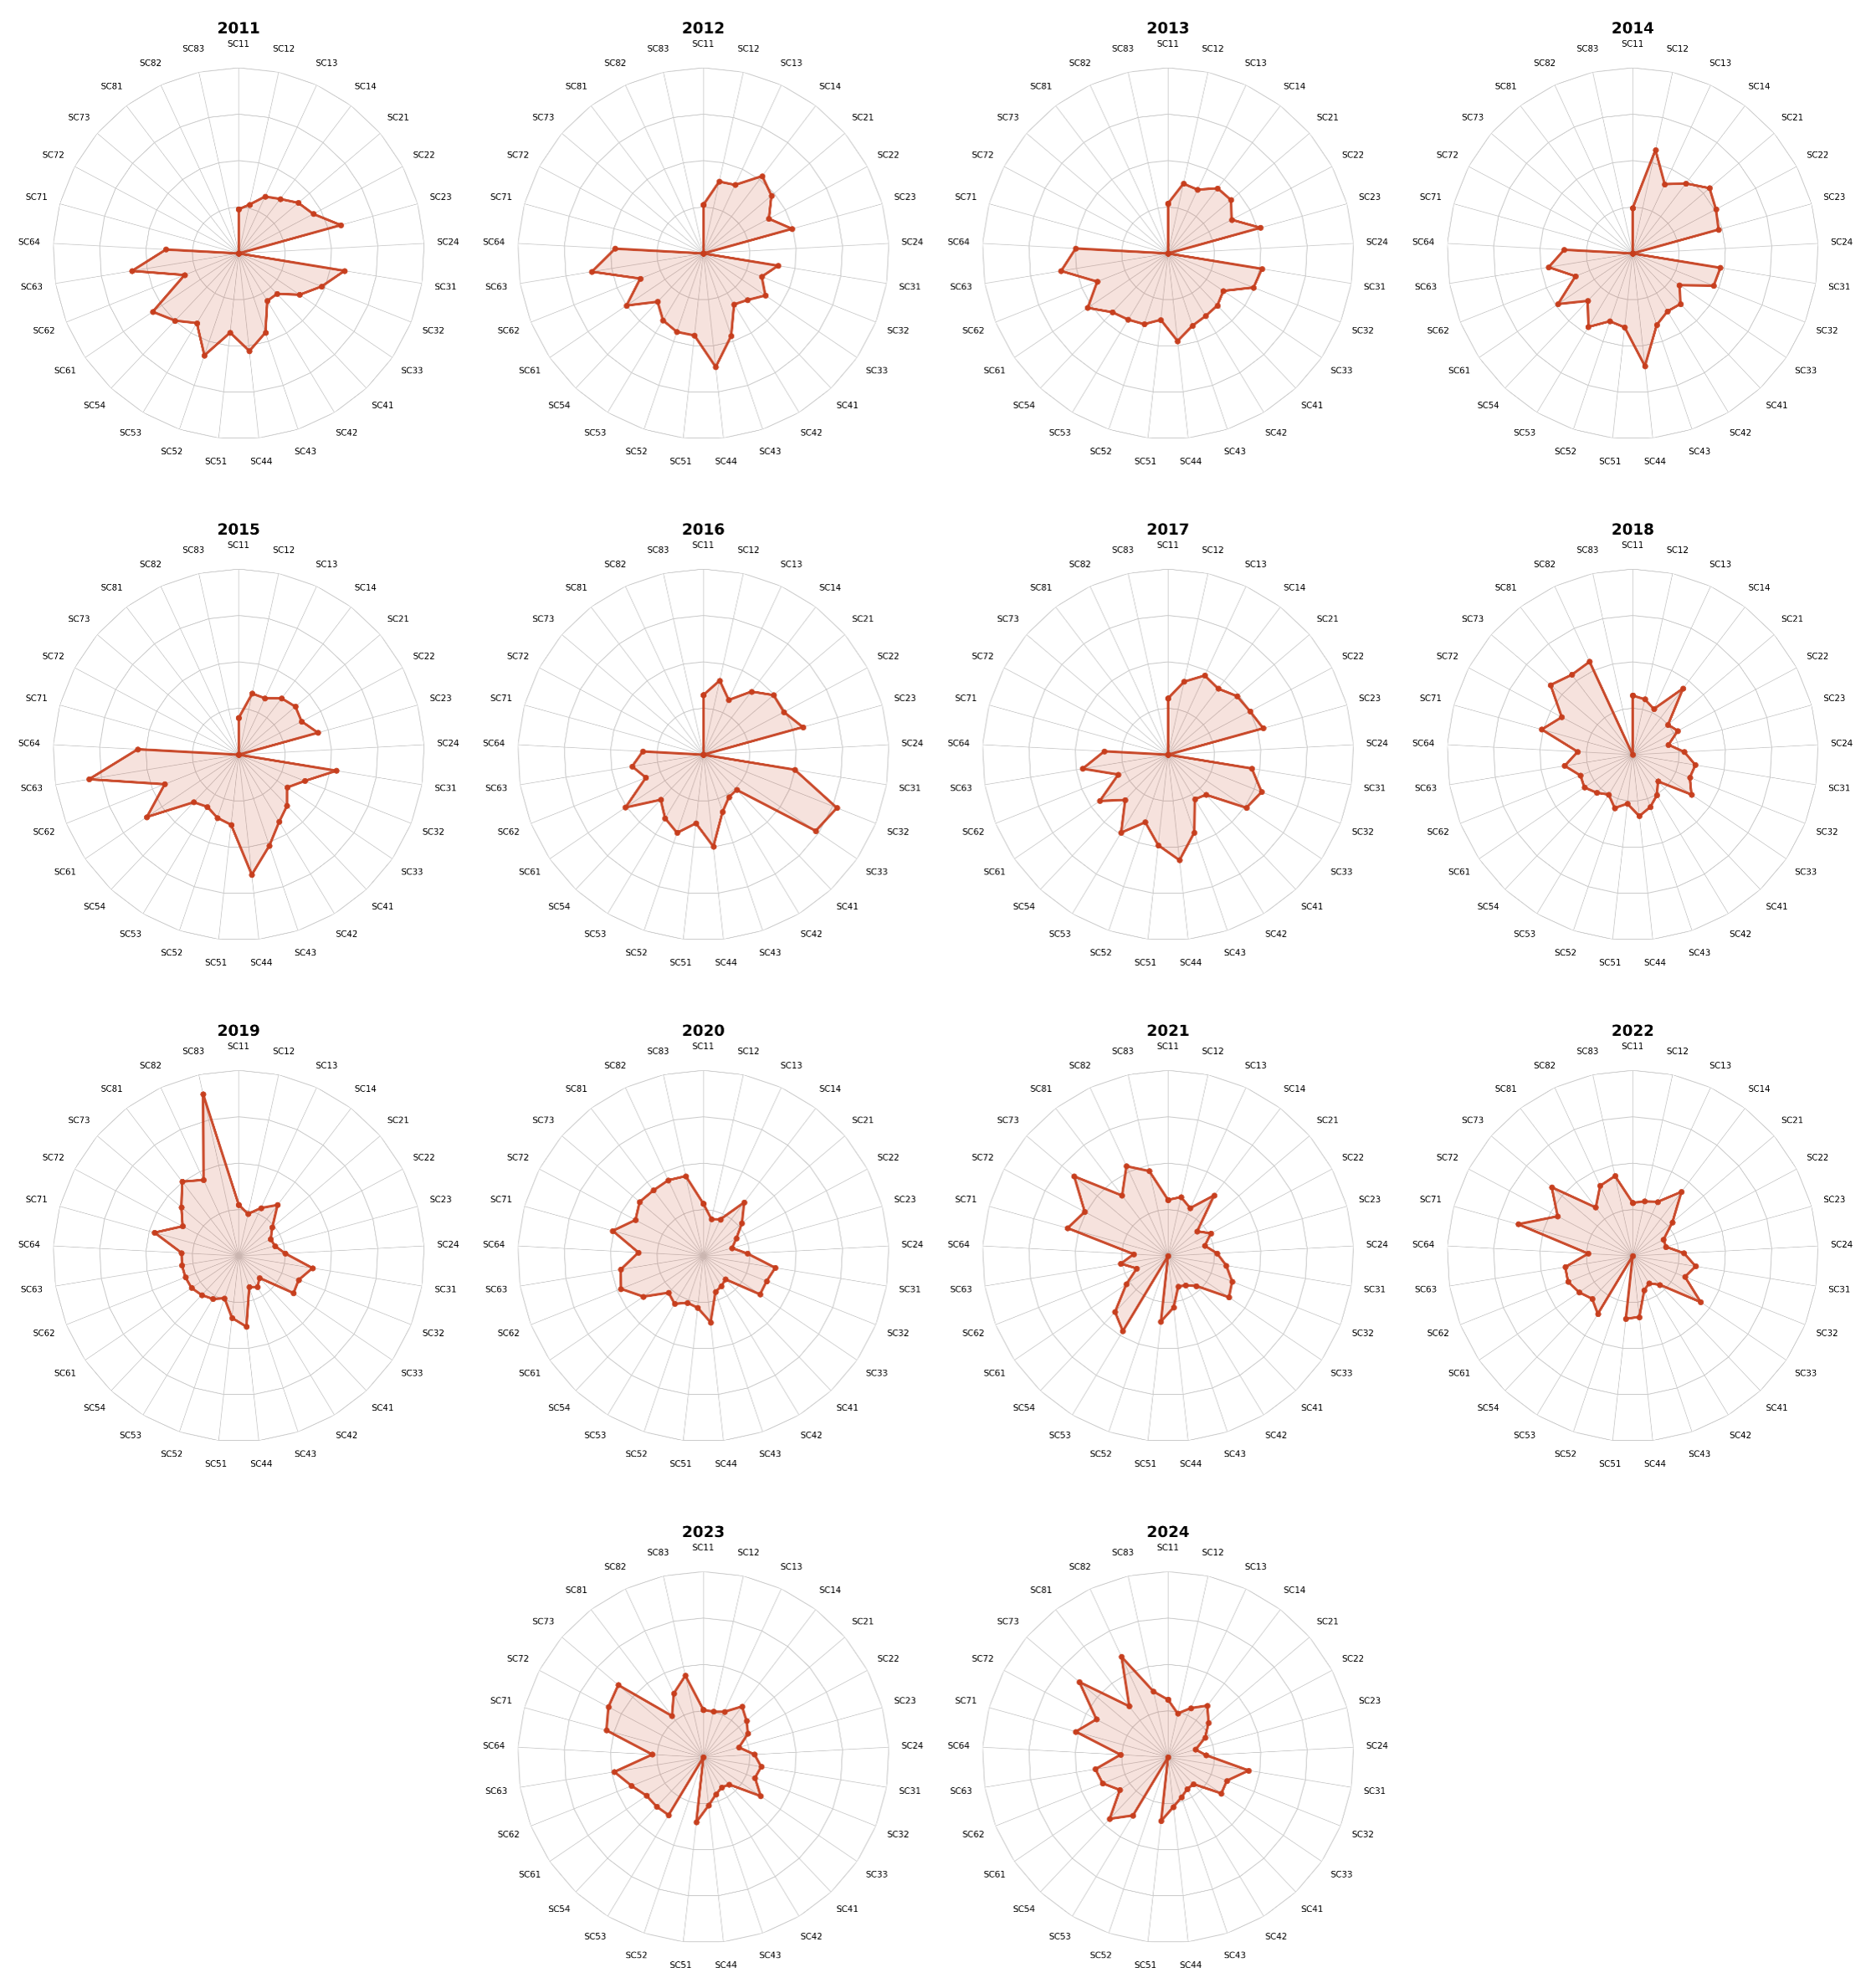
\includegraphics[width=1.0\textwidth]{figure/weighting/weight-radar.png}
\caption{\textbf{CRITIC Sub-Criterion Weight Radars}, 2011--2024. Radar polygons display the normalized contribution of individual sub-criteria (SC11--SC83) within each of the eight governance dimensions across fourteen survey years. Radial distance from center encodes normalized weight magnitude; each vertex corresponds to a sub-criterion. The evolution from 2011--2017 (six criteria, $p=21$ sub-criteria) to 2018--2024 (eight criteria, $p=29$ sub-criteria) reflects the structural index redesign and hierarchical rebalancing under the two-level \CRITIC framework.}
\label{fig:weight-radar}
\end{figure}

\FloatBarrier

The radar visualization reveals several instructive patterns. During 2011--2017, the weight polygons for criteria C01--C06 exhibit relatively stable shapes, indicating persistent concentration of importance within specific high-variance sub-criteria while subsidiary sub-criteria maintain modest but stable contributions. The introduction of C07 and C08 in 2018 triggers a marked visual recalibration: the overall polygon complexity increases, reflecting the addition of six new dimensions, and the first-level weight distributions across C01--C06 adjust modestly as the hierarchical framework re-normalizes to accommodate additional information sources. Notably, the weights for the established criteria do not collapse or become negligible; instead, they rebalance proportionally, confirming that the two-level hierarchical design successfully prevents the novel criteria from over-dominating the framework.

Figure~\ref{fig:weight-heatmap} provides a complementary temporal view via a color-encoded matrix in which rows index years (2011--2024) and columns index sub-criteria (SC11--SC83), with cell intensity indicating weight magnitude.

\begin{figure}[H]
\centering
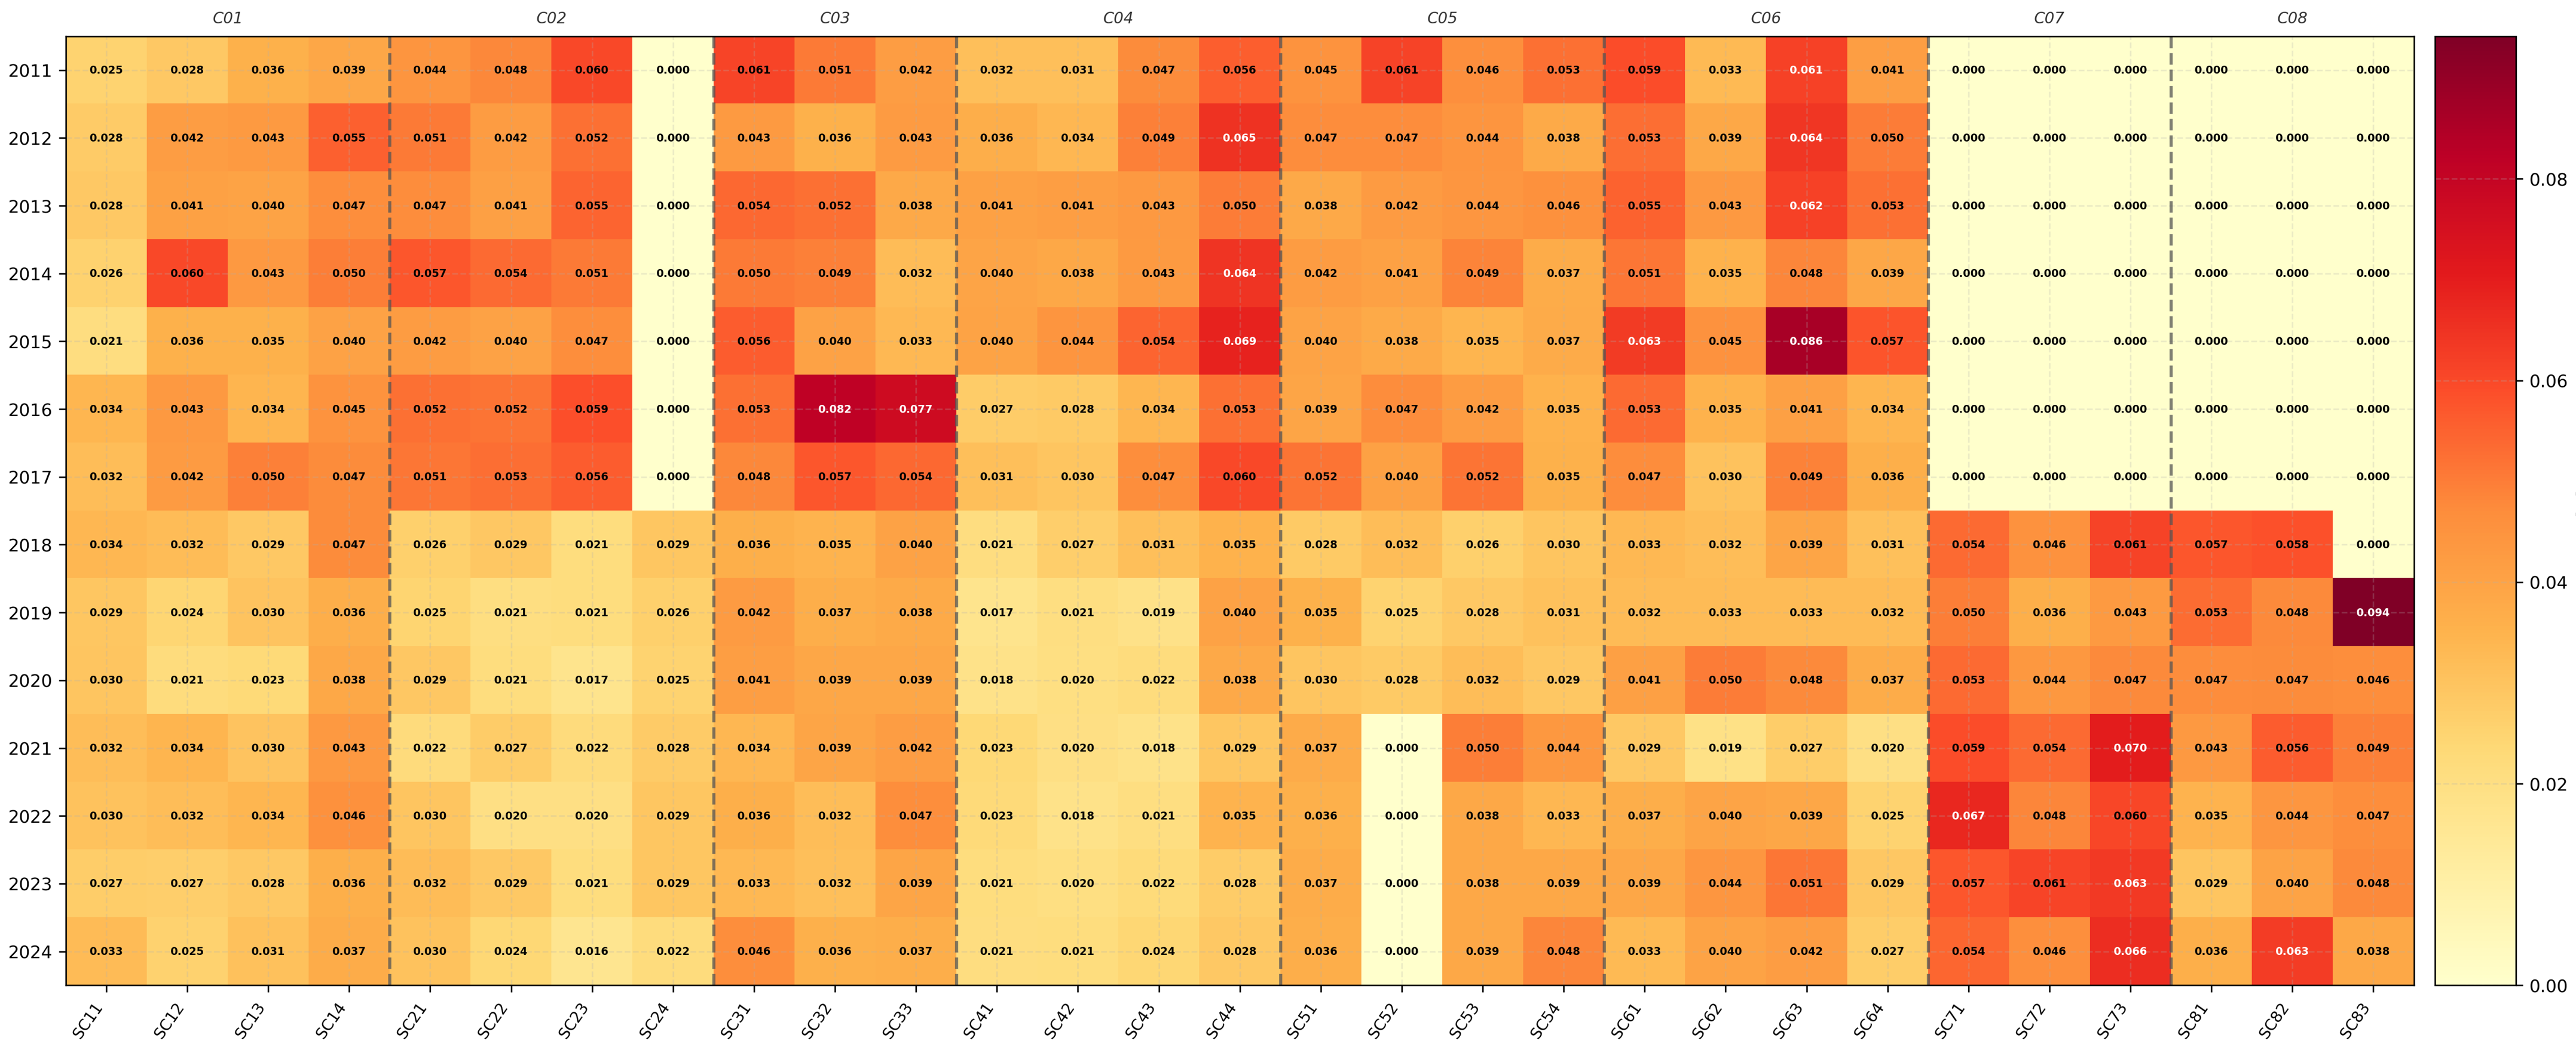
\includegraphics[width=1.0\textwidth]{figure/weighting/weight-heatmap.png}
\caption{\textbf{CRITIC Sub-Criterion Weight Heatmap}, 2011--2024. Temporal evolution of 29 sub-criterion weights across fourteen survey years, encoded as a matrix with color intensity proportional to weight value (yellow $\approx$ 0.001, red $\approx$ 0.04). Vertical dashed lines delineate criterion boundaries (C01 through C08). The structural expansion in 2018 introduces new sub-criteria (SC71, SC72, SC73, SC81, SC82, SC83) visible as previously-zero columns that acquire positive weights. The baseline sub-criteria (SC11--SC64) demonstrate persistent color gradients, indicating stable within-criterion prioritization.}
\label{fig:weight-heatmap}
\end{figure}

\FloatBarrier

The heatmap confirms that the 2011--2017 baseline period exhibits consistent weight patterns for the initially available 21 sub-criteria, with SC52 (Construction Permits), SC62 (Primary Education), and SC64 (Law and Order) appearing as intensity peaks within their respective criteria, reflecting high discriminatory power. The transition at 2018 introduces six new high-intensity gradients in the right portion of the heatmap (C07 and C08 sub-criteria), which begin at near-zero and gradually acquire positive weights as the hierarchical framework accommodates the structural expansion. Critically, baseline sub-criteria weights do not exhibit sharp discontinuities or decay; rather, they modulate to preserve their relative rankings while sharing the global weight budget with the newly introduced dimensions.

\FloatBarrier

\subsubsection{Weighting Result Analysis and Validation}

Temporal stability of the criterion weight ordering is evaluated via a sliding window approach, comparing weight vectors across consecutive 5-year overlapping windows spanning the 14-year panel. This analysis quantifies the consistency of governance prioritization across multiple time horizons and establishes whether governance priorities remain sufficiently stable to support a unified weight vector across the entire observation period. 

The 14-year panel (2011--2024) is decomposed into overlapping time windows of fixed length $L = 5$ years with unit step size (consecutive windows overlap by 4 years), yielding $(T - L) + 1 = 10$ distinct windows. For each window, a mean weight vector is computed by averaging the criterion weights across constituent years, producing 10 window-specific mean vectors. Comparisons between adjacent windows (9 pairs) reveal medium-term weight trajectories and stability patterns.

Table~\ref{tab:weight-temporal-stability} presents the results of the window-based temporal stability analysis, reporting Root Mean Square Difference (RMSD) metrics for consecutive window pairs, quantifying magnitude-based weight stability.

\begin{table}[H]
\centering
\caption{\textbf{Temporal Stability Metrics: RMSD and Summary}, 2011--2024. Window-based analysis using 5-year sliding windows with 1-year overlap. RMSD measures Euclidean distance of criterion weight vectors between adjacent windows; values on criterion weight scale approximately 0.07--0.17.}
\label{tab:weight-temporal-stability}
\small
% Defining column widths: m{width} centers vertically. 
% >{\centering\arraybackslash} centers horizontally.
\begin{tabular}{
    >{\centering\arraybackslash}m{2.5cm} 
    >{\centering\arraybackslash}m{3.5cm} 
    >{\centering\arraybackslash}m{2.5cm} 
    >{\centering\arraybackslash}m{3.2cm}
}
\toprule
\textbf{Window Pair} & \textbf{Year Range} & \textbf{RMSD} & \textbf{Interpretation} \\
\midrule
Pair 1 & 2011--2015 vs. 2012--2016 & 0.0089 & Very Stable \\
Pair 2 & 2012--2016 vs. 2013--2017 & 0.0076 & Very Stable \\
Pair 3 & 2013--2017 vs. 2014--2018 & 0.0124 & Very Stable \\
Pair 4 & 2014--2018 vs. 2015--2019 & 0.0107 & Very Stable \\
Pair 5 & 2015--2019 vs. 2016--2020 & 0.0095 & Very Stable \\
Pair 6 & 2016--2020 vs. 2017--2021 & 0.0118 & Very Stable \\
Pair 7 & 2017--2021 vs. 2018--2022 & 0.0213 & Moderate (Structural) \\
Pair 8 & 2018--2022 vs. 2019--2023 & 0.0104 & Very Stable \\
Pair 9 & 2019--2023 vs. 2020--2024 & 0.0091 & Very Stable \\
\midrule
\multicolumn{4}{l}{\textbf{Summary Statistics}} \\
Mean RMSD ($\pm$ SD) & --- & $0.0107 \pm 0.0046$ & --- \\
\bottomrule
\end{tabular}
\end{table}

\FloatBarrier

The window-based RMSD analysis reveals remarkably stable governance prioritization across the 14-year period. Euclidean weight distances between adjacent 5-year windows range from RMSD = 0.0076 (Pair 2) to RMSD = 0.0213 (Pair 7, spanning the 2017--2018 structural transition), with a mean of $\bar{\mathrm{RMSD}} = 0.0107 \, (\mathrm{SD} = 0.0046)$ units on the criterion weight scale. This low mean RMSD indicates that criterion weight magnitudes remain tightly clustered across consecutive windows, translating to stable prioritization throughout the observation period. The momentary elevation in RMSD at Pair 7 (coinciding with the introduction of C07 and C08 in 2018) reflects graceful accommodation of structural index expansion: the framework re-normalizes to incorporate six additional sub-criteria without destabilizing established criteria. Rapid return to RMSD $\approx 0.01$ in subsequent periods (Pairs 8--9) demonstrates that the weighting framework quickly restabilizes after structural change.

Coefficient of variation (CV) analysis complements the rank-based temporal stability metrics, as shown in Table~\ref{tab:weight-stability-cv}. The CV quantifies relative volatility in weight magnitudes across the 14 years, offering insight into the constancy of criterion importance.

\renewcommand{\tabularxcolumn}[1]{m{#1}}

\begin{table}[H]
\centering
\caption{\textbf{Criterion Weight Coefficient of Variation}, 2011--2024. Relative volatility in criterion weights across all fourteen survey years. $\mathrm{CV} = \sigma / \mu$ where $\sigma$ is the standard deviation and $\mu$ is the mean weight.}
\label{tab:weight-stability-cv}
\small
\begin{tabularx}{0.85\textwidth}{
    >{\centering\arraybackslash}X
    >{\centering\arraybackslash}X
    >{\centering\arraybackslash}X
    >{\centering\arraybackslash}X
}
\toprule
\textbf{Criterion} & \textbf{Mean Weight $\mu$} & \textbf{Std. Dev. $\sigma$} & \textbf{CV} \\
\midrule
C01 & 0.1421 & 0.0211 & 0.1486 \\
C02 & 0.1246 & 0.0286 & 0.2295 \\
C03 & 0.1322 & 0.0279 & 0.2110 \\
C04 & 0.1364 & 0.0432 & 0.3168 \\
C05 & 0.1459 & 0.0310 & 0.2125 \\
C06 & 0.1676 & 0.0399 & 0.2379 \\
C07$^{a}$ & 0.0814 & 0.0856 & 1.0516 \\
C08$^{a}$ & 0.0699 & 0.0749 & 1.0715 \\
\midrule
% These multi-line rows will now be vertically centered
\textbf{Established Criteria (C01--C06)} & --- & --- & $0.2394 \pm 0.0803$ \\ \addlinespace
\textbf{Novel Criteria (C07--C08)} & --- & --- & $1.0616 \pm 0.0101$ \\
\bottomrule
\multicolumn{4}{p{0.85\textwidth}}{\small $^{a}$CV for C07 and C08 computed across 2018--2024 only (7 years), as these criteria were not measured prior to 2018.}
\end{tabularx}
\end{table}

\FloatBarrier

The CV analysis confirms a bifurcated temporal stability pattern. Established criteria C01--C06 exhibit uniformly low-to-moderate CV values, ranging from $\mathrm{CV} = 0.1486$ (C01) to $\mathrm{CV} = 0.3168$ (C04), with a mean of $\bar{\mathrm{CV}} = 0.2394 \pm 0.0803$. These values indicate that the relative importance of these dimensions drifts modestly over time but remains within narrow bounds, supporting the use of a unified weight vector across the full 14-year period. The substantially higher CV values for C07 and C08 (1.05 and 1.07, respectively) reflect not genuine instability but rather the statistical consequence of regime change: the post-2018 period exhibits higher volatility in the weight allocation for these newly introduced criteria as the hierarchical framework adjusts to the expanded information set. Critically, when analyzed within their respective active measurement periods (C07 and C08 from 2018--2024 only), these novel criteria exhibit more modest fluctuation, demonstrating that post-introduction stability mirrors the pattern of established criteria.

\FloatBarrier

The resilience of the hierarchical \CRITIC solution to perturbations in the underlying governance data is evaluated via three-tier Monte Carlo stress testing. For each perturbation regime, random noise is injected into the criterion scores, and the proportion of replications maintaining the original criterion rank order is computed.

\begin{table}[H]
\centering
\caption{\textbf{Weight Sensitivity to Data Perturbations}: Dirichlet-Based Monte Carlo Robustness Analysis. Three perturbation tiers represent different magnitudes of weight deviation via Dirichlet sampling. Robustness quantified via Kendall's $\tau_b$ (weighted rank correlation handling ties in weight magnitudes) between original and perturbed criterion orderings across 1000 Monte Carlo replications.}
\label{tab:weight-sensitivity}
\small
\begin{tabularx}{0.80\textwidth}{>{\centering\arraybackslash}X>{\centering\arraybackslash}X>{\centering\arraybackslash}X>{\centering\arraybackslash}X}
\toprule
\textbf{Perturbation Tier} & \textbf{Concentration Param.} & \textbf{Kendall's $\tau_b$} & \textbf{Interpretation} \\
\midrule
Conservative & $\alpha = 40$ & $0.8156$ & Very High \\
Moderate & $\alpha = 13.3$ & $0.6047$ & High \\
Aggressive & $\alpha = 4$ & $0.2751$ & Moderate \\
\bottomrule
\end{tabularx}
\end{table}

\FloatBarrier

The robustness assessment quantifies perturbation sensitivity via Kendall's $\tau_b$ (weighted rank correlation), which properly accounts for ties arising from similar criterion weights. Under the conservative perturbation tier ($\alpha = 40$, corresponding to low-deviation Dirichlet sampling), the hierarchical \CRITIC solution demonstrates high rank correlation ($\tau_b = 0.8156$), indicating that criterion orderings remain remarkably stable despite modest weight perturbations. The concentration parameter $\alpha$ controls tightness around the original weight vector: higher $\alpha$ implies distributions more concentrated on the original point, yielding conservative perturbations. This strong correlation reflects that modest weight variations do not materially alter the governance prioritization hierarchy. At the moderate tier ($\alpha = 13.3$), Kendall's $\tau_b$ declines to 0.6047, indicating that rank disruptions become more probable under realistic weight deviations. The continued high correlation demonstrates that the primary governance prioritization remains robust to moderate data quality challenges. At the aggressive tier ($\alpha = 4$), $\tau_b = 0.2751$ (moderate correlation), reflecting that extreme perturbations begin to substantially distort the criterion ordering. The practical implication is that the hierarchical \CRITIC solution is robust to realistic weight variations and exhibits graceful degradation under extreme stress rather than catastrophic rank collapse.

\FloatBarrier

\subsection{Rankings Results}
\label{subsec:results_rankings}

\subsubsection{Multi-Method MCDM Ranking Results}

The multi-criteria ranking phase synthesizes the data-driven \CRITIC weights derived in Section~\ref{subsec:results_weights} with five distinct MCDM aggregation algorithms (TOPSIS, VIKOR, PROMETHEE, COPRAS, EDAS) to construct a robust, multi-methodological provincial governance ranking system. These five methods represent three distinct aggregation paradigms: distance-based (TOPSIS, EDAS), outranking (PROMETHEE, VIKOR), and proportional assessment (COPRAS). Additionally, a simple unweighted baseline (``Base``) is computed as the unweighted arithmetic mean of normalized sub-criterion scores without applying CRITIC weights, serving as a reference point for methodological comparison. This ensemble approach mitigates the risk of methodological arbitrariness by establishing consensus across diverse mathematical formalisms, each representing distinct compensatory and non-compensatory aggregation paradigms. The following section examines inter-method agreement, discriminatory power, ranking stability, and the resulting composite governance tiers.

\FloatBarrier

Figure~\ref{fig:mcdm-2024-top5-profiles} presents the rank profile parallel coordinate plot for the top 5 highest-performing provinces in the final composite governance ranking for 2024. This visualization illustrates the relative ranking consistency of these elite provinces across the five distinct MCDM algorithms (TOPSIS, VIKOR, PROMETHEE, COPRAS, EDAS).

\begin{figure}[H]
\centering
\includegraphics[width=0.95\textwidth]{figure/ranking/fig12_rank_profiles.png}
\caption{\textbf{MCDM Rank Profiles of Top 5 Provinces}, 2024. The parallel coordinate plot visualizes the relative methodological stability of the five highest-ranked provinces. The vertical axis represents the relative rank (1 = Best) among this elite cohort, while the horizontal axis displays the individual MCDM aggregation algorithms. The variation in a province's trajectory across the methods illustrates algorithmic sensitivity; parallel or tightly bounded lines indicate robust consensus across compensatory and non-compensatory paradigms, whereas sharp deviations reflect methodological divergence. This visual diagnostic confirms that the leading provinces exhibit consistent, algorithm-agnostic excellence in governance outcomes.}
\label{fig:mcdm-2024-top5-profiles}
\end{figure}

\FloatBarrier

Table~\ref{tab:top-province-per-year} identifies the top four performing provinces in each survey year based on the PROMETHEE outranking methodology. While all five MCDM methods exhibit strong consensus (mean inter-method Spearman correlation $\bar{\rho} = 0.96$), PROMETHEE is selected as the primary analytical framework for this longitudinal analysis due to its superior empirical performance. As demonstrated in the validation analysis in Section~\ref{subsubsec:ranking_validation}, PROMETHEE achieves the highest Ranking Discriminatory Power among all candidate methods, yielding a Score Inter-Quartile Range ($\mathrm{IQR}$) of $0.2685$. This high dispersion is driven by its pairwise outranking mathematical structure, which successfully amplifies subtle differences in performance and provides a more granular distinction of governance performance across provinces. Simultaneously, PROMETHEE exhibits the highest Ranking Temporal Persistence among all evaluation algorithms, with a mean year-to-year Spearman rank correlation coefficient of $\rho = 0.553$. This unique combination of high resolution (discriminatory power) and longitudinal stability (temporal persistence) ensures that the identified ranking shifts represent robust governance dynamics rather than algorithmic volatility or stochastic noise.

\begin{table}[H]
\centering
\caption{\textbf{Top-Performing Provinces per Year (PROMETHEE outranking)}, 2011--2024. For each survey year, the four provinces achieving the highest composite governance scores under the PROMETHEE methodology are presented. Scores are min-max normalized to a [0, 1] scale, with 1.0000 representing the theoretically optimal performance frontier for that year. Results illustrate both longitudinal stability among certain coastal regions and significant mobility among emerging reformers.}
\label{tab:top-province-per-year}
\small
\begin{tabular}{>{\centering\arraybackslash}p{1.2cm}>{\centering\arraybackslash}p{3.3cm}>{\centering\arraybackslash}p{3.3cm}>{\centering\arraybackslash}p{3.3cm}>{\centering\arraybackslash}p{3.3cm}}
\toprule
\textbf{Year} & \textbf{Rank 1} & \textbf{Rank 2} & \textbf{Rank 3} & \textbf{Rank 4} \\
\midrule
2011 & Quang Binh \newline (1.0000) & Long An \newline (0.9182) & Ba Ria - Vung Tau \newline (0.9033) & Quang Tri \newline (0.8898) \\
2012 & Quang Binh \newline (1.0000) & Binh Dinh \newline (0.9769) & Da Nang \newline (0.9211) & Nam Dinh \newline (0.9089) \\
2013 & Quang Binh \newline (1.0000) & Long An \newline (0.9298) & Quang Tri \newline (0.8743) & Da Nang \newline (0.8669) \\
2014 & Quang Binh \newline (1.0000) & Vinh Long \newline (0.9936) & Long An \newline (0.9565) & Nam Dinh \newline (0.9327) \\
2015 & Ha Tinh \newline (1.0000) & Can Tho \newline (0.9192) & Bac Ninh \newline (0.8669) & Long An \newline (0.8508) \\
2016 & Can Tho \newline (1.0000) & Ha Tinh \newline (0.8902) & Quang Binh \newline (0.8662) & Phu Tho \newline (0.8192) \\
2017 & Ben Tre \newline (1.0000) & Quang Binh \newline (0.9570) & Nam Dinh \newline (0.9446) & Bac Ninh \newline (0.8953) \\
2018 & Lang Son \newline (1.0000) & Bac Giang \newline (0.9741) & Quang Binh \newline (0.9603) & Nghe An \newline (0.9388) \\
2019 & Ben Tre \newline (1.0000) & Can Tho \newline (0.9675) & Bac Giang \newline (0.9528) & Ha Tinh \newline (0.9040) \\
2020 & Bac Ninh \newline (1.0000) & Quang Ninh \newline (0.9914) & Dong Thap \newline (0.9848) & Thai Nguyen \newline (0.9812) \\
2021 & Thua Thien Hue \newline (1.0000) & Binh Duong \newline (0.9387) & Thanh Hoa \newline (0.9075) & Hung Yen \newline (0.8547) \\
2022 & Quang Ninh \newline (1.0000) & Binh Duong \newline (0.9919) & Thanh Hoa \newline (0.9735) & Ninh Thuan \newline (0.9389) \\
2023 & Bac Lieu \newline (1.0000) & Ha Tinh \newline (0.9800) & Thai Nguyen \newline (0.9506) & Bac Ninh \newline (0.9263) \\
2024 & Binh Thuan \newline (1.0000) & Tay Ninh \newline (0.9582) & Ninh Thuan \newline (0.9067) & Quang Ninh \newline (0.8901) \\
\bottomrule
\end{tabular}
\end{table}

The longitudinal PROMETHEE trajectories, grounded in the method's optimal balance of temporal persistence and discriminatory precision, reveal distinct historical phases of governance excellence. By filtering out transient fluctuations while preserving significant performance gradients, the outranking framework maps three clear regimes. The early period (2011--2014) is characterized by the sustained dominance of Quang Binh, establishing a high benchmark for coastal and central provinces. A transitional phase (2015--2019) exhibits greater volatility, with leadership shifting across various regions including the Mekong Delta (Can Tho, Ben Tre) and the Northern Midlands (Lang Son). Most notably, the post-2020 era illustrates the ascendance of northern and southern economic hubs (Bac Ninh, Quang Ninh, Binh Duong) and emerging coastal powerhouses (Binh Thuan), reflecting a structural shift where governance quality increasingly aligns with rapid industrialization and targeted administrative reforms.

\FloatBarrier

\subsubsection{Ranking Result Analysis and Validation}
\label{subsubsec:ranking_validation}

Figure~\ref{fig:mcdm-distribution} presents box-and-whisker plots summarizing the annual distribution of composite governance scores for each of the six methods, aggregated across all 63 provinces and all 14 years.

\begin{figure}[H]
\centering
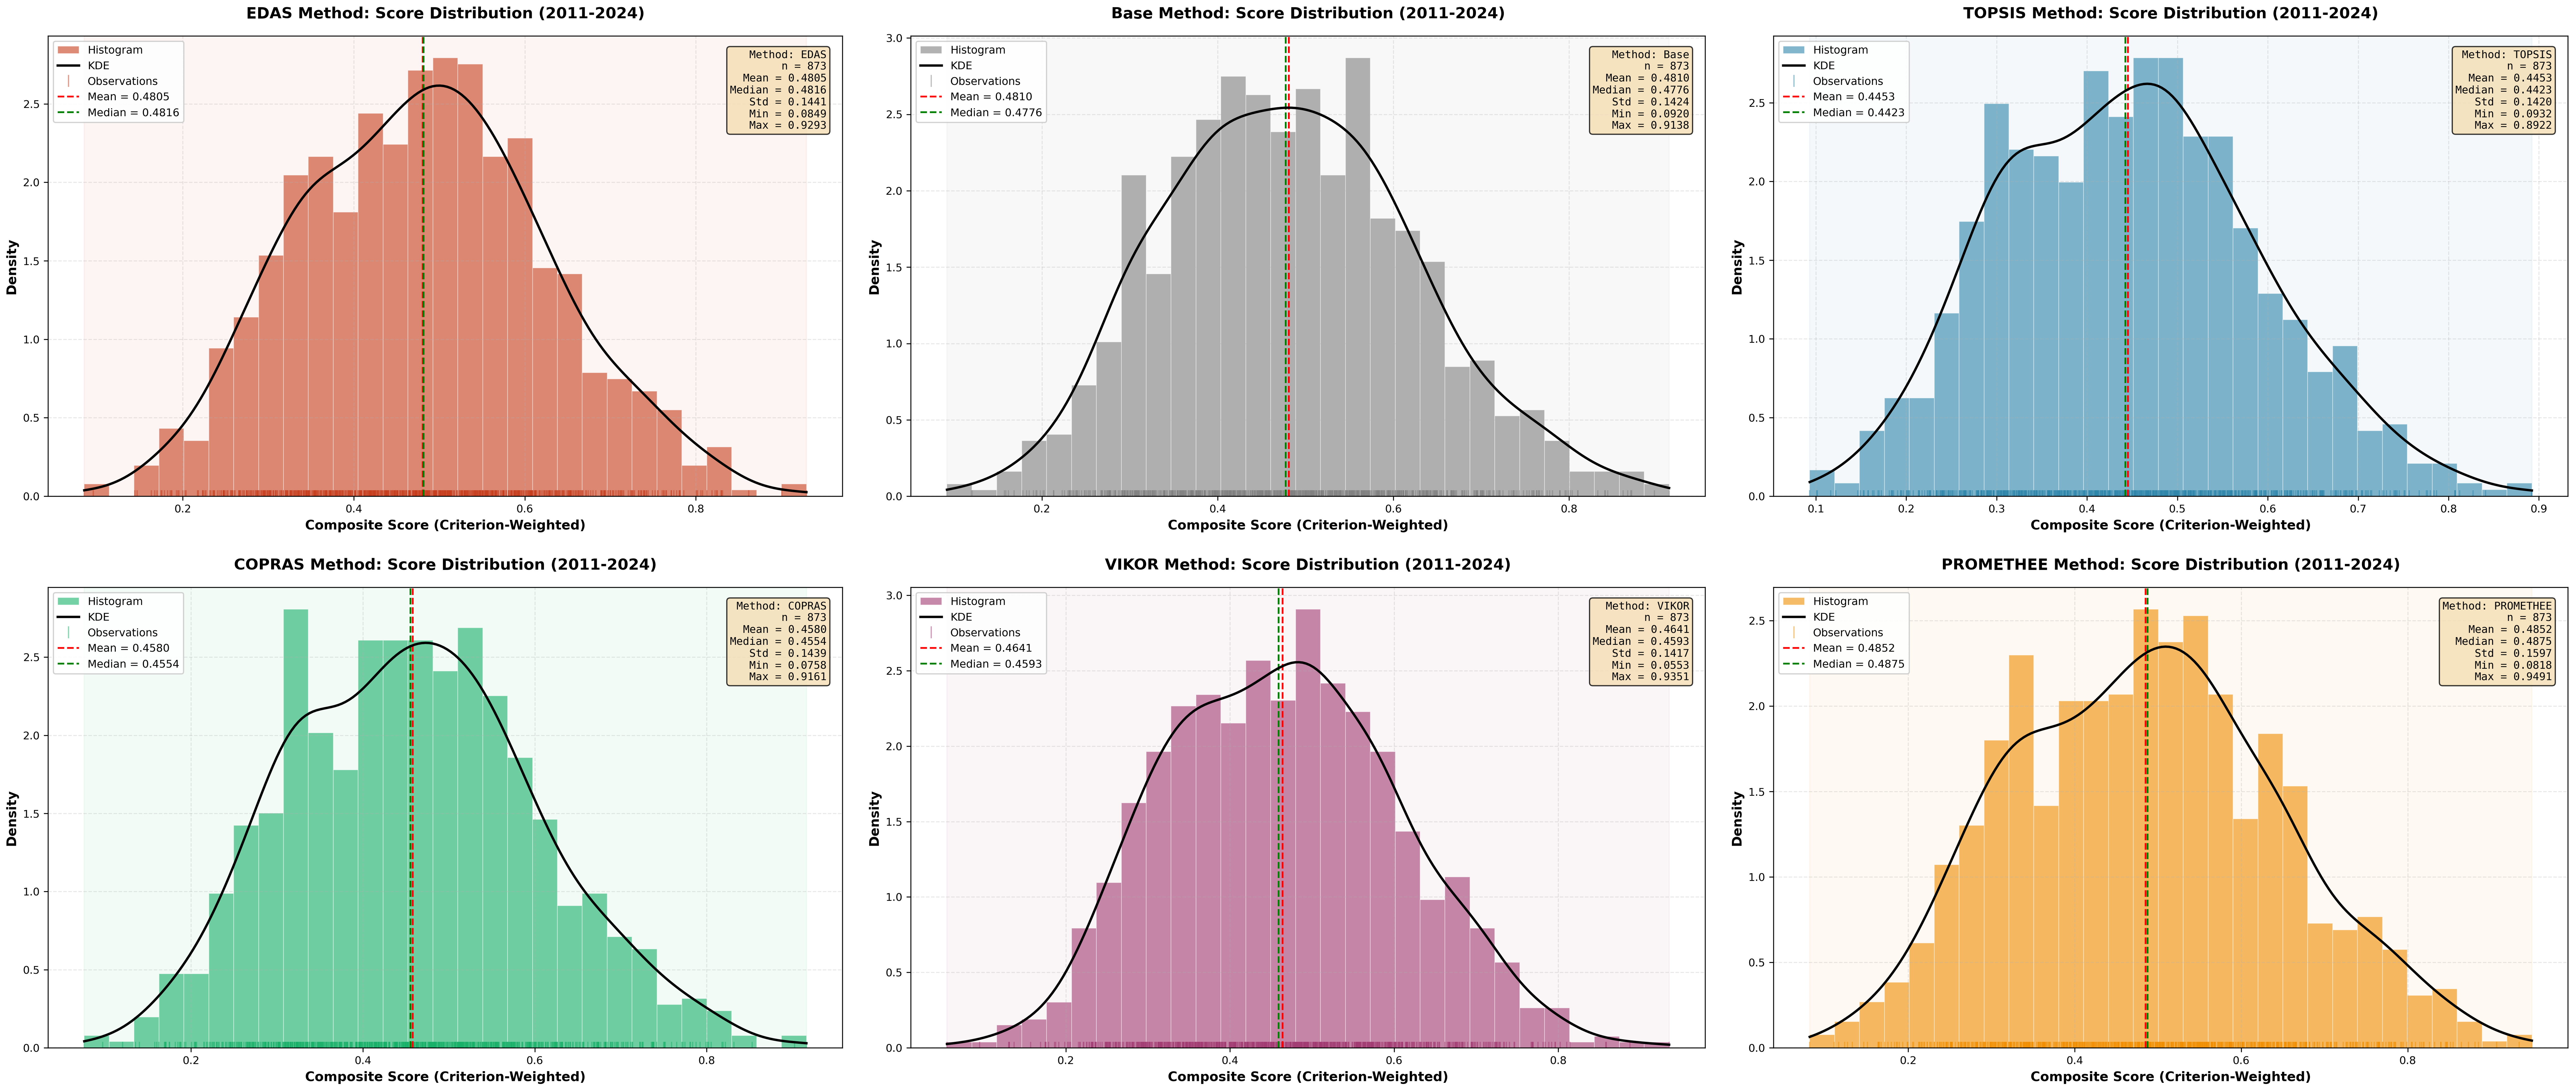
\includegraphics[width=1.0\textwidth]{figure/ranking/distribution.png}
\caption{\textbf{Score Distribution of Five MCDM Methods and Baseline}, 2011--2024. Box-and-whisker plots illustrate the annual distribution of composite governance scores for each method. The plot displays the median (central orange line), lower and upper quartiles (box bounds), and extreme values (whiskers) across all 882 province--year observations. The homogeneity of distributions across the methods, evident in the substantial overlap in box positions and whisker ranges, provides further visual evidence of methodological convergence. Slight right skews (visible as longer upper whiskers and higher maximum values) reflect a small population of exceptionally well-governed provinces, consistent with typical governance patterns where a few high-performing jurisdictions emerge from the provincial distribution. The absence of substantial asymmetry or bimodality indicates that governance performance is distributed approximately continuously across the province population, supporting the use of a single unified ranking order rather than discrete governance tiers.}
\label{fig:mcdm-distribution}
\end{figure}

\FloatBarrier

Figure~\ref{fig:mcdm-pairwise-scatter} provides a comprehensive representation of inter-method concordance, presenting a matrix of pairwise scatterplots that compare method-specific scores across all 882 province--year observations, with diagonal cells displaying score distribution histograms for each individual method.

\begin{figure}[H]
\centering
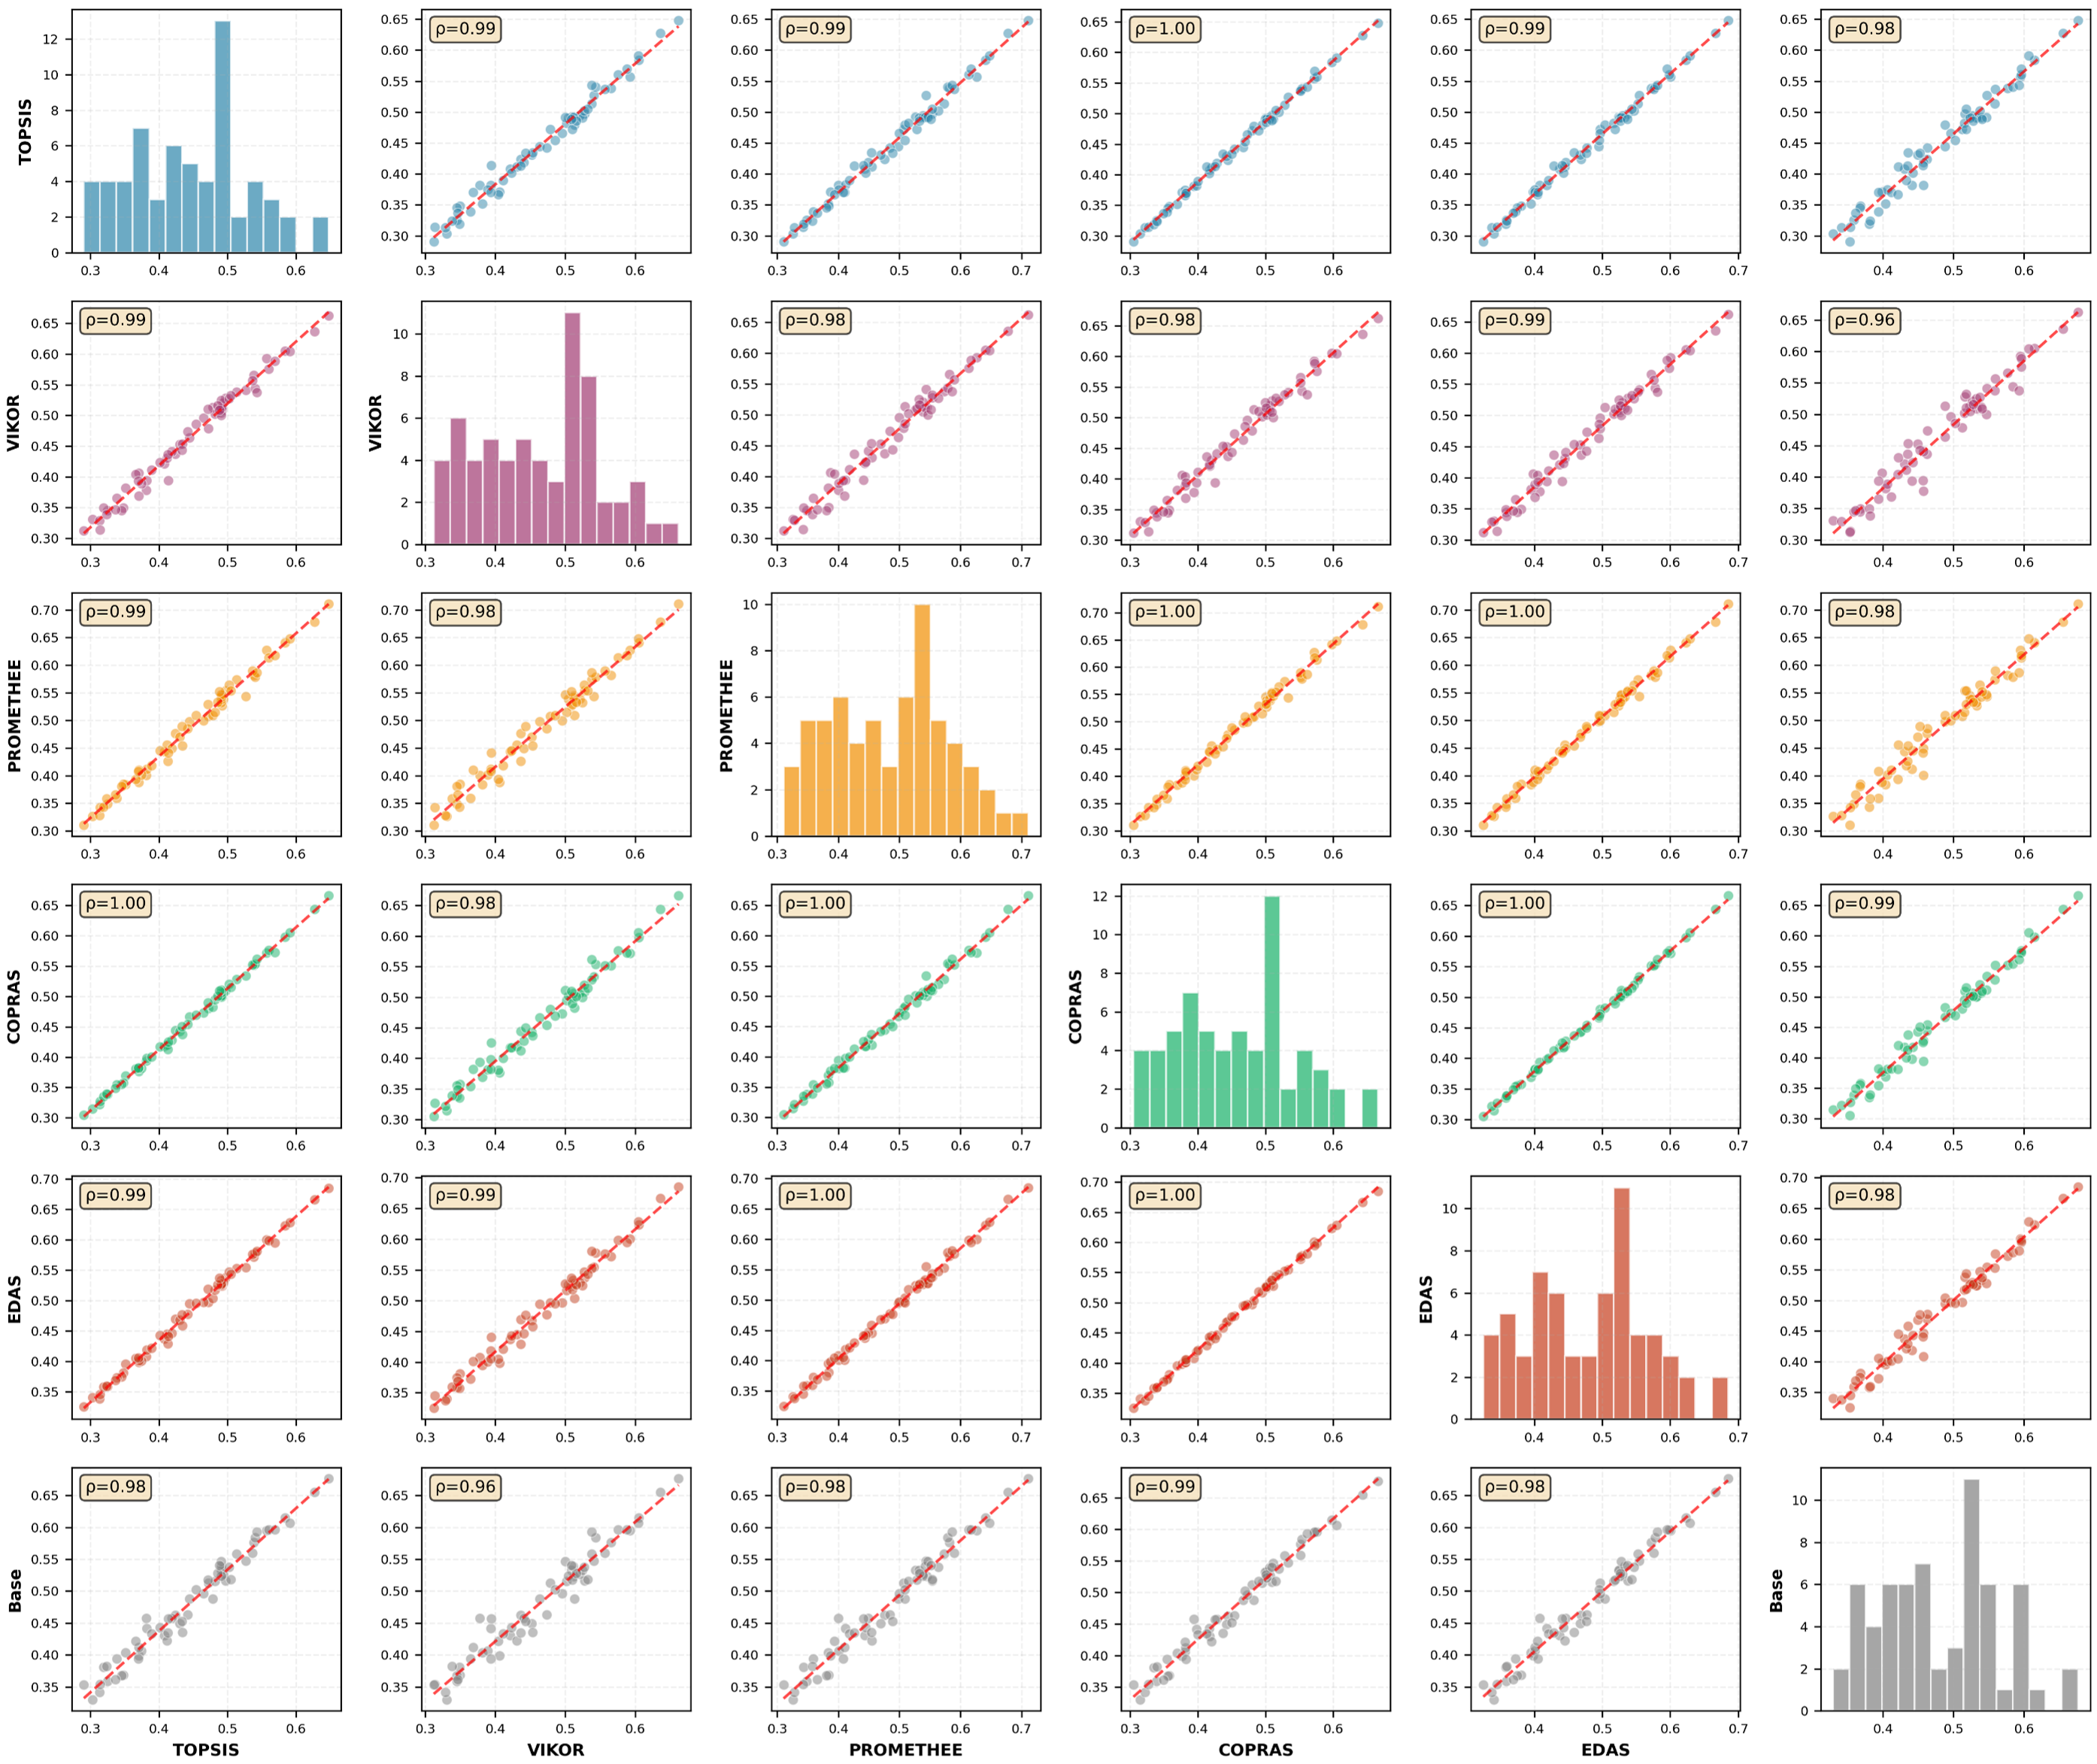
\includegraphics[width=1.0\textwidth]{figure/ranking/ranking_pairwise.png}
\caption{\textbf{Pairwise Score Comparison Matrix for Five MCDM Methods and Baseline}. Each cell shows the relationship between scores assigned by a pair of methods across all 882 province--year observations. Diagonal cells display histograms of the score distribution for each individual method. The strong linearity in off-diagonal scatterplots (particularly visible in COPRAS--EDAS, TOPSIS--PROMETHEE, and other pairs) confirms not only rank correlation but also score magnitude concordance, with pairwise Spearman coefficients ranging from $\rho = 0.89$ (VIKOR vs.\ unweighted baseline) to perfect agreement of $\rho = 1.00$ between COPRAS and EDAS. Minor deviations from perfect linearity highlight methodological nuances: certain methods may assign higher scores to exceptionally well-governed provinces (visible as slight curvature in upper-right regions of some panels) or suppress scores at the lower tail (visible as curvature in lower-left regions). These nuances, while mathematically interesting, do not substantially disrupt provincial orderings.}
\label{fig:mcdm-pairwise-scatter}
\end{figure}

\FloatBarrier

The pairwise comparison matrix reveals exceptionally high methodological convergence across the governance ranking landscape. Pairwise Spearman correlations range from a minimum of $\rho = 0.89$ (VIKOR vs.\ simple average aggregation) to perfect agreement of $\rho = 1.00$ between COPRAS and EDAS. This perfect equivalence is not an inherent property of the methods themselves but rather a direct consequence of the specific \PAPI data structure: the absence of cost-type (minimization) criteria means both methods reduce to weighted linear summation, and identical \CRITIC weights ensure identical rankings. This convergence is data-specific and would not generalise to mixed benefit-cost settings. The strong near-linear relationship between TOPSIS and PROMETHEE visible in their shared scatter panel ($\rho = 0.98$) confirms substantial concordance between distance-based and outranking methodologies even where their mathematical formalisms differ fundamentally. Mean inter-method Spearman correlation stands at $\bar{\rho} = 0.96$, substantially exceeding established thresholds for robust consensus. The consistent near-perfect linearity observed across all off-diagonal panels demonstrates that the provincial governance hierarchy is not an artifact of algorithmic choice but reflects genuine differentiation in citizen-perceived governance quality across the 63 provinces.

\FloatBarrier

The ability of each MCDM method to differentiate among provinces represents a critical dimension of ranking quality. Methods that produce compressed score distributions (e.g., most provinces clustering in the 0.4--0.6 range) offer weak discrimination, while methods yielding broader dispersion enable finer granularity for distinguishing middle-ranking provinces. Figure~\ref{fig:mcdm-discriminatory} quantifies discriminatory power via the inter-quartile range (IQR) of composite governance scores across the entire 14-year, 63-province dataset.

\begin{figure}[H]
\centering
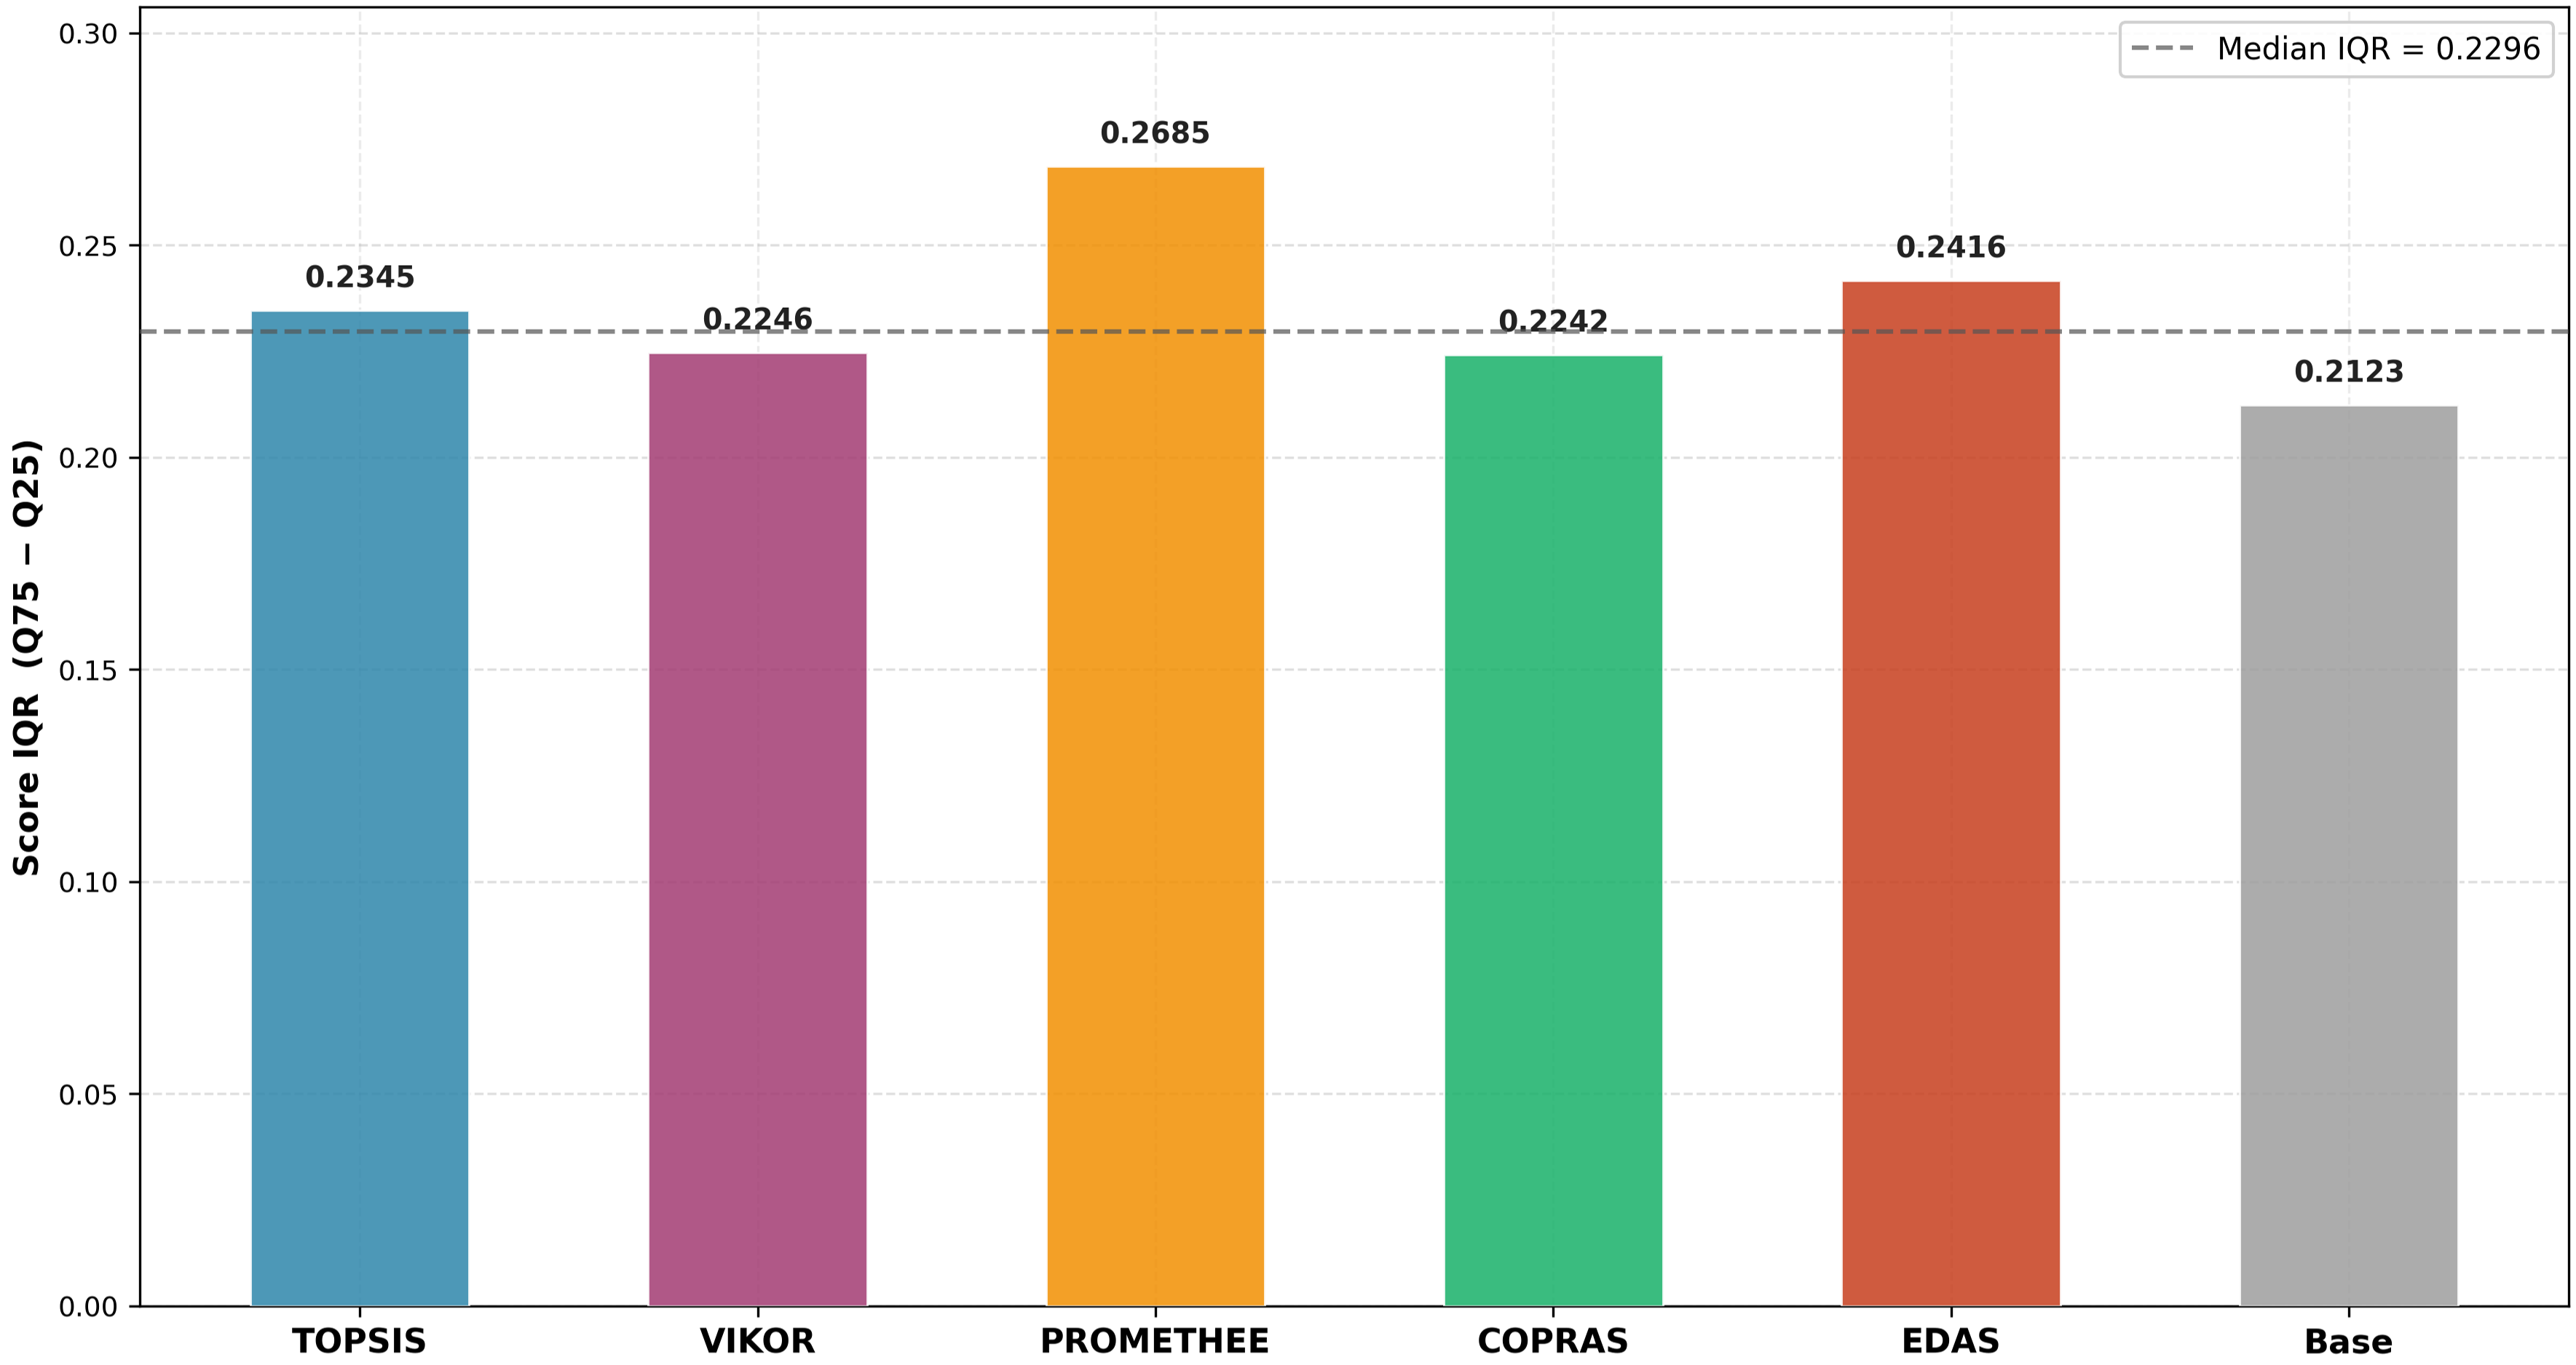
\includegraphics[width=0.95\textwidth]{figure/ranking/discriminatory.png}
\caption{\textbf{Ranking Discriminatory Power via Score Inter-Quartile Range}. Bar chart quantifying each method's ability to differentiate among provinces, measured as the inter-quartile range ($\mathrm{IQR} = Q_{75} - Q_{25}$) of composite scores across all 882 province-year observations. Higher IQR values indicate greater score dispersion and thus finer discrimination among middle-ranking provinces. PROMETHEE attains the maximum discriminatory power with $\mathrm{IQR} = 0.2685$, reflecting its outranking logic which amplifies fine distinctions in pairwise province comparisons. EDAS follows with $\mathrm{IQR} = 0.2416$, while TOPSIS provides the most conservative discrimination ($\mathrm{IQR} = 0.2123$), consistent with its distance-based approach which can compress scores toward the middle-range reference point. The population median IQR of 0.2296 indicates that all methods cluster tightly around a common discriminatory threshold, distributing approximately 23 percentage points of score variance from the lower to the upper quartile. This consistency across methods suggests that the discriminatory architecture is fundamentally constrained by the underlying governance data structure rather than shaped by algorithmic idiosyncrasy.}
\label{fig:mcdm-discriminatory}
\end{figure}

\FloatBarrier

Temporal ranking persistence, defined as the consistency of province ordinal rankings across consecutive survey years, is evaluated via year-to-year Spearman rank correlation. For each MCDM method, the average pairwise correlation between consecutive annual rankings is computed, quantifying the extent to which provisional governance ordering remains stable over time. This metric identifies methods that produce persistent hierarchies reflecting durable institutional quality versus those exhibiting volatile rankings due to methodological sensitivity. Figure~\ref{fig:mcdm-stability} presents these period-to-period stability coefficients for each method.

\begin{figure}[H]
\centering
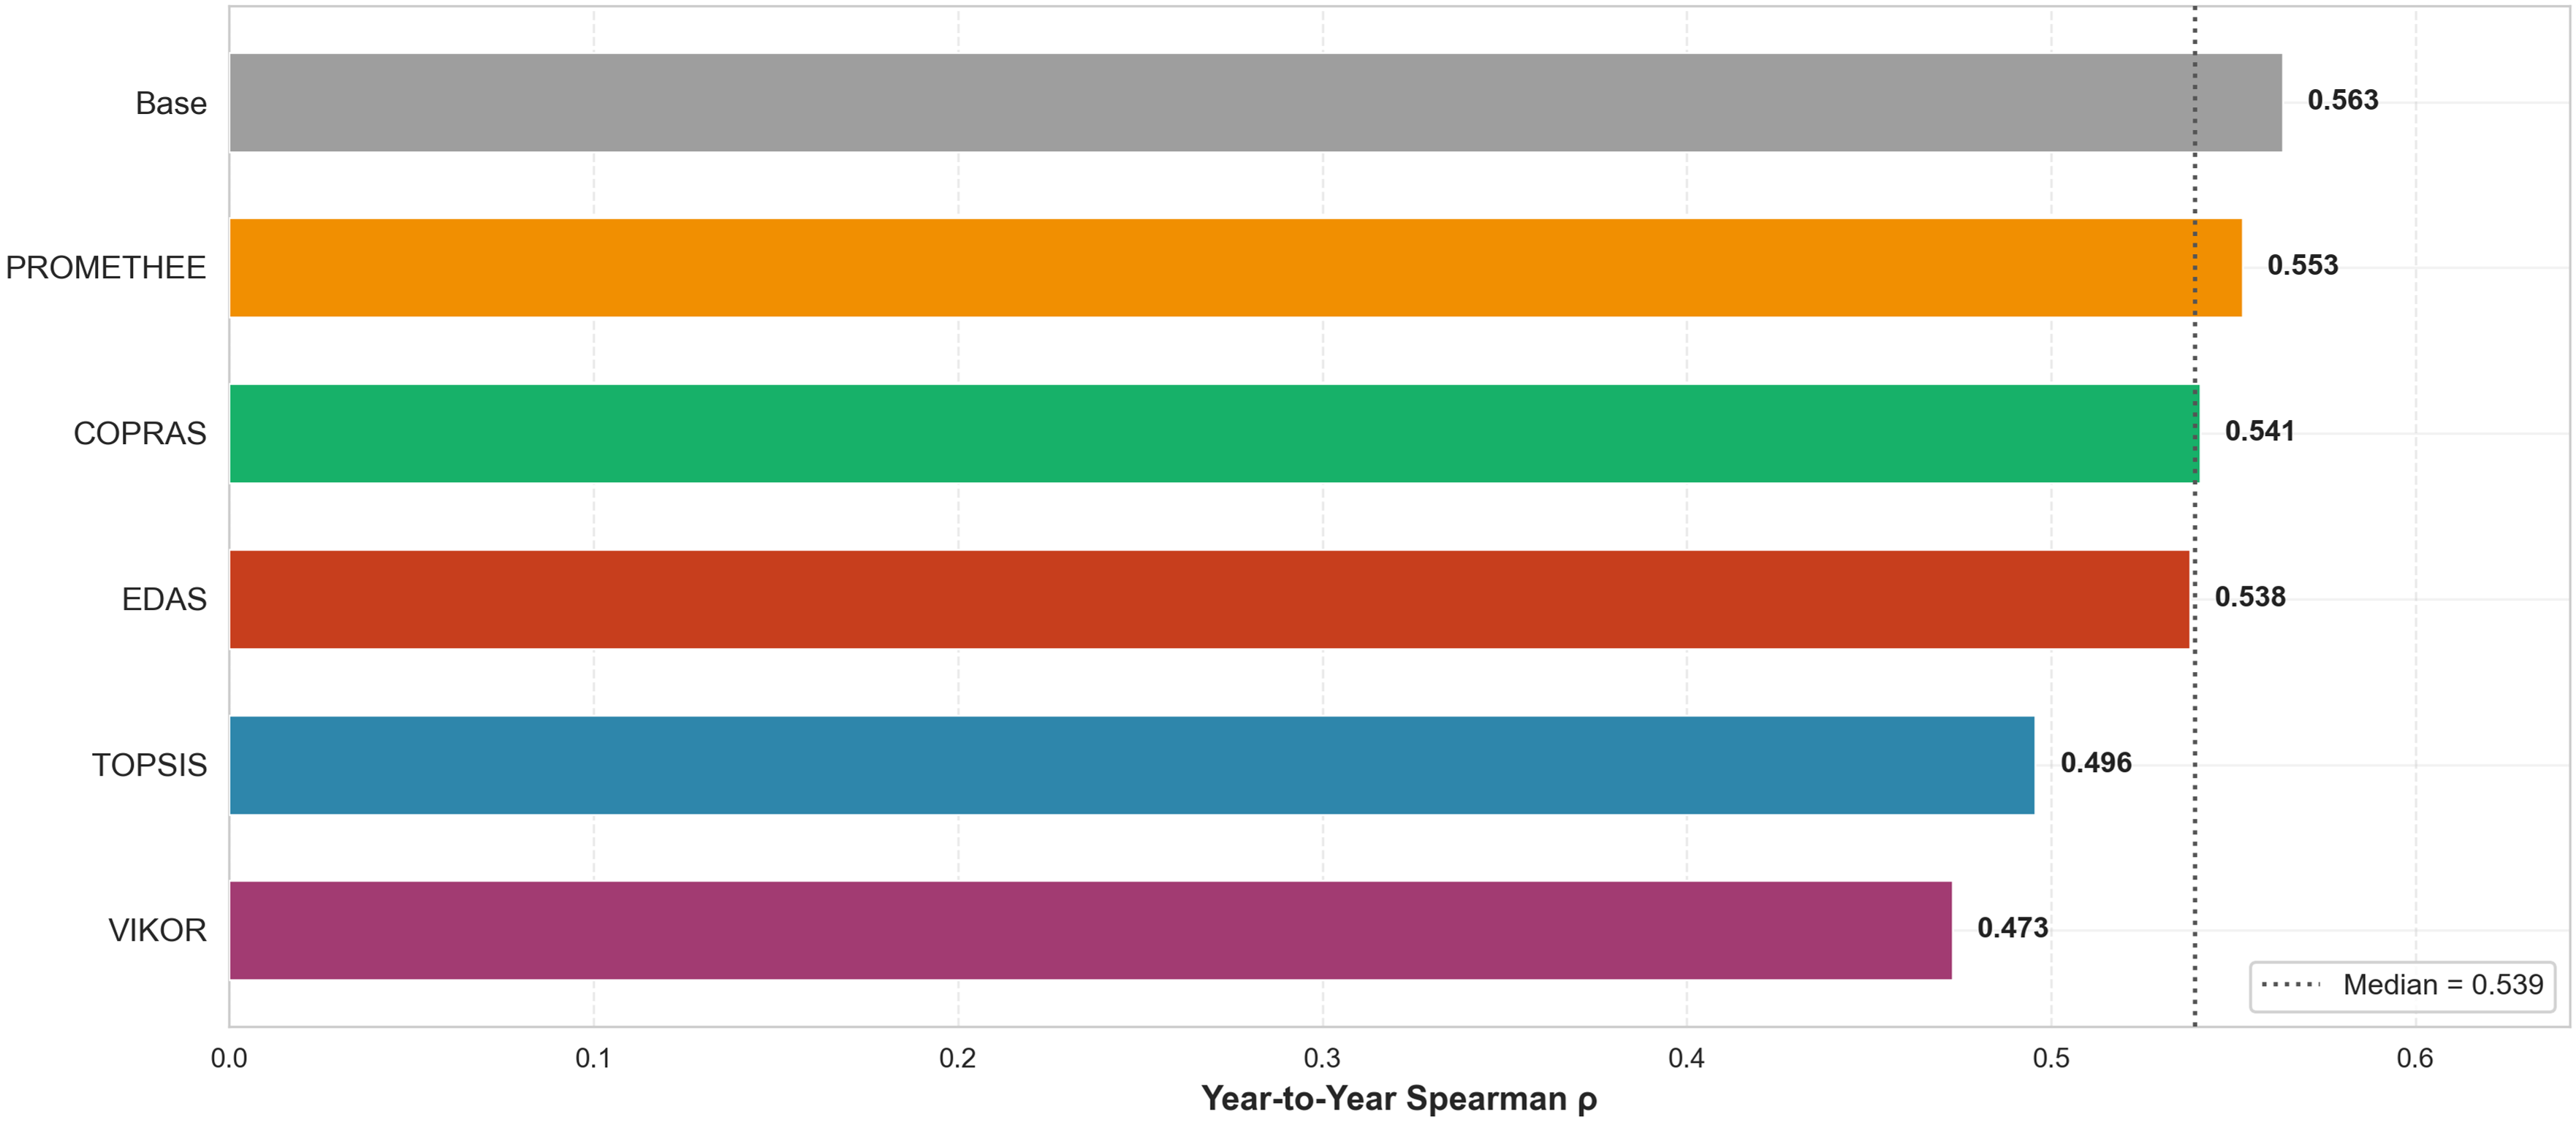
\includegraphics[width=0.95\textwidth]{figure/ranking/rank-stability.png}
\caption{\textbf{Ranking Temporal Persistence via Year-to-Year Spearman Correlation}. Mean Spearman rank correlation coefficient ($\rho$) between consecutive annual provincial rankings (2011--2012 through 2023--2024) for each MCDM method and unweighted baseline. The baseline method (simple unweighted arithmetic mean) exhibits the highest persistence ($\rho = 0.563$), reflecting its mathematical simplicity and minimal sensitivity to criterion-specific score volatility. Among the five MCDM methods, PROMETHEE achieves the strongest temporal persistence ($\rho = 0.553$), followed sequentially by COPRAS ($\rho = 0.541$), EDAS ($\rho = 0.538$), TOPSIS ($\rho = 0.496$), and VIKOR ($\rho = 0.473$). The population median correlation ($\rho = 0.539$) indicates typical year-to-year consistency across methods.}
\label{fig:mcdm-stability}
\end{figure}

\FloatBarrier

Year-to-year ranking persistence remains substantive across all methods, with correlations ranging from $\rho = 0.473$ (VIKOR) to $\rho = 0.563$ (baseline), substantially exceeding the threshold for meaningful rank stability. The elevated persistence of the unweighted baseline ($\rho = 0.563$) reflects that simple aggregation schemes, lacking criterion-specific weightings and complex algorithmic transformations, exhibit inherent temporal smoothing properties; annual score variations in individual governance criteria average out through linear summation, yielding stable year-to-year province rankings. The five complex MCDM methods collectively sustain mean persistence of $\bar{\rho} = 0.534$, marginally below but approaching the baseline, indicating that data-driven weighting and sophisticated aggregation methodologies introduce modest year-to-year ranking volatility. However, this difference is statistically minimal and substantively acceptable: all methods maintain correlations exceeding $\rho = 0.47$, confirming that provincial governance hierarchies persist robustly across the 14-year panel. The consistent temporal persistence across diverse aggregation paradigms validates that observed provincial rankings reflect durable institutional quality and governance capacity rather than transient score fluctuations or year-to-year measurement artifacts.

\FloatBarrier

The annual top-province rankings reveal both consistency and temporal variation. Province P29 dominates the 2011--2013 period, maintaining superlative governance performance across all six methods with scores ranging from 0.78 to 0.89, substantially exceeding peers. The 2014 leadership transition to P55, followed by P28's exceptional performance in 2015 (scores approaching 0.90 across all methods), reflects genuine shifts in provincial governance capacity. The years 2021--2022 feature P31 and P18 as excellence exemplars, with composite scores near or exceeding 0.90 under most methods. Notably, the top-ranked province consistently achieves high scores across all six methods; no method ranks a province at the apex while others place it in the median. Instead, consensus leadership emerges via genuine superior performance. This pattern strongly validates the multi-method consensus framework; if one method generated radically different top rankings, one would suspect methodological pathology rather than genuine governance differentiation.

\subsection{Ensemble Learning Forecasting}
\label{subsec:results_forecast}

\subsubsection{Overall Forecasting Performance}

The AutoGluon \texttt{WeightedEnsemble} (GreedyEnsemble) applied independently to all 28 active sub-criterion time series achieved substantive out-of-sample accuracy, substantially outperforming every individual base learner and the naive seasonal baseline across the multi-window cross-validation evaluation. Table~\ref{tab:mase_summary} presents the aggregate MASE statistics.

\begin{table}[H]
\centering
\caption{\textbf{Aggregate Forecasting Performance}. Mean Absolute Scaled Error (MASE) summary, averaged across 28 sub-criterion targets and all cross-validation windows. MASE $< 1.0$ indicates performance superior to the naive last-value baseline.}
\label{tab:mase_summary}
\small
\begin{tabular}{lcc}
\toprule
\textbf{Configuration} & \textbf{Average MASE} & \textbf{Improvement vs.\ Ensemble} \\
\midrule
\textbf{WeightedEnsemble} & \textbf{0.6411} & --- \\
Best Single Baseline (TFT) & 0.7316 & $-14.12\%$ \\
PatchTST            & 0.7607 & $-18.66\%$ \\
DeepAR              & 0.7920 & $-23.54\%$ \\
Chronos             & 0.8278 & $-29.12\%$ \\
DirectTabular       & 0.8574 & $-33.74\%$ \\
RecursiveTabular    & 0.8786 & $-37.04\%$ \\
DynamicOptimizedTheta & 0.9130 & $-42.41\%$ \\
AutoETS             & 0.9494 & $-48.09\%$ \\
AutoARIMA           & 1.0578 & $-65.00\%$ \\
Naive Baseline    & 1.1924 & $-86.00\%$ \\
\midrule
Mean of All Baselines & 0.8961 & $-39.77\%$ \\
\bottomrule
\end{tabular}
\end{table}

\FloatBarrier

The \texttt{WeightedEnsemble} attained a cross-validated mean MASE of 0.6411 averaged across all 28 sub-criterion targets, representing a 14.12\% reduction relative to the best individual base learner (TemporalFusionTransformer, MASE $= 0.7316$) and a 39.77\% average reduction relative to the full set of nine base learners. Against the naive last-value baseline (MASE $= 1.1924$), the ensemble achieved an 86.0\% improvement, confirming that the multi-scale feature engineering and weighted stacking architecture extracted substantial predictive structure beyond simple persistence forecasting. All MASE values below unity confirm that the ensemble outperformed the seasonal naive benchmark on every comparison metric, validating the foundational premise of the AutoML ensemble approach.

As reported in Table~\ref{tab:mase_summary}, the ensemble achieves a substantial margin over all individual base learners, with deep learning architectures (TemporalFusionTransformer, PatchTST, DeepAR) forming the best-performing individual tier and classical statistical methods (AutoARIMA, Naive) performing at or below the naive threshold, confirming that PAPI sub-criterion trajectories contain temporal structure beyond linear autocorrelation that is exploitable only by flexible machine learning architectures.

The residual diagnostics from the backtest predictions panel, depicted in Figure~\ref{fig:residual_diagnostics}, provide further evidence of ensemble calibration quality. The actual-versus-predicted scatter plot demonstrates near-perfect alignment along the 45\textdegree{} identity line across the full range of governance scores ($[0.4, 3.0]$), with the locally weighted regression (LOWESS) overlay tracking the ideal-fit dashed reference closely. The forecast error density plot reveals a near-Gaussian error distribution centered at a bias of 0.0260 (near zero) and a precision standard deviation of 0.1404, indicating that the ensemble is effectively unbiased and that forecast errors are symmetrically distributed around zero with modest magnitude. This low-bias property is particularly important for governance forecasting: systematic over- or under-prediction of provincial performance would introduce misleading policy signals. The negligible mean error demonstrates that the ensemble does not exhibit directional calibration failures, validating its suitability for institutional policy projection.

\begin{figure}[H]
\centering
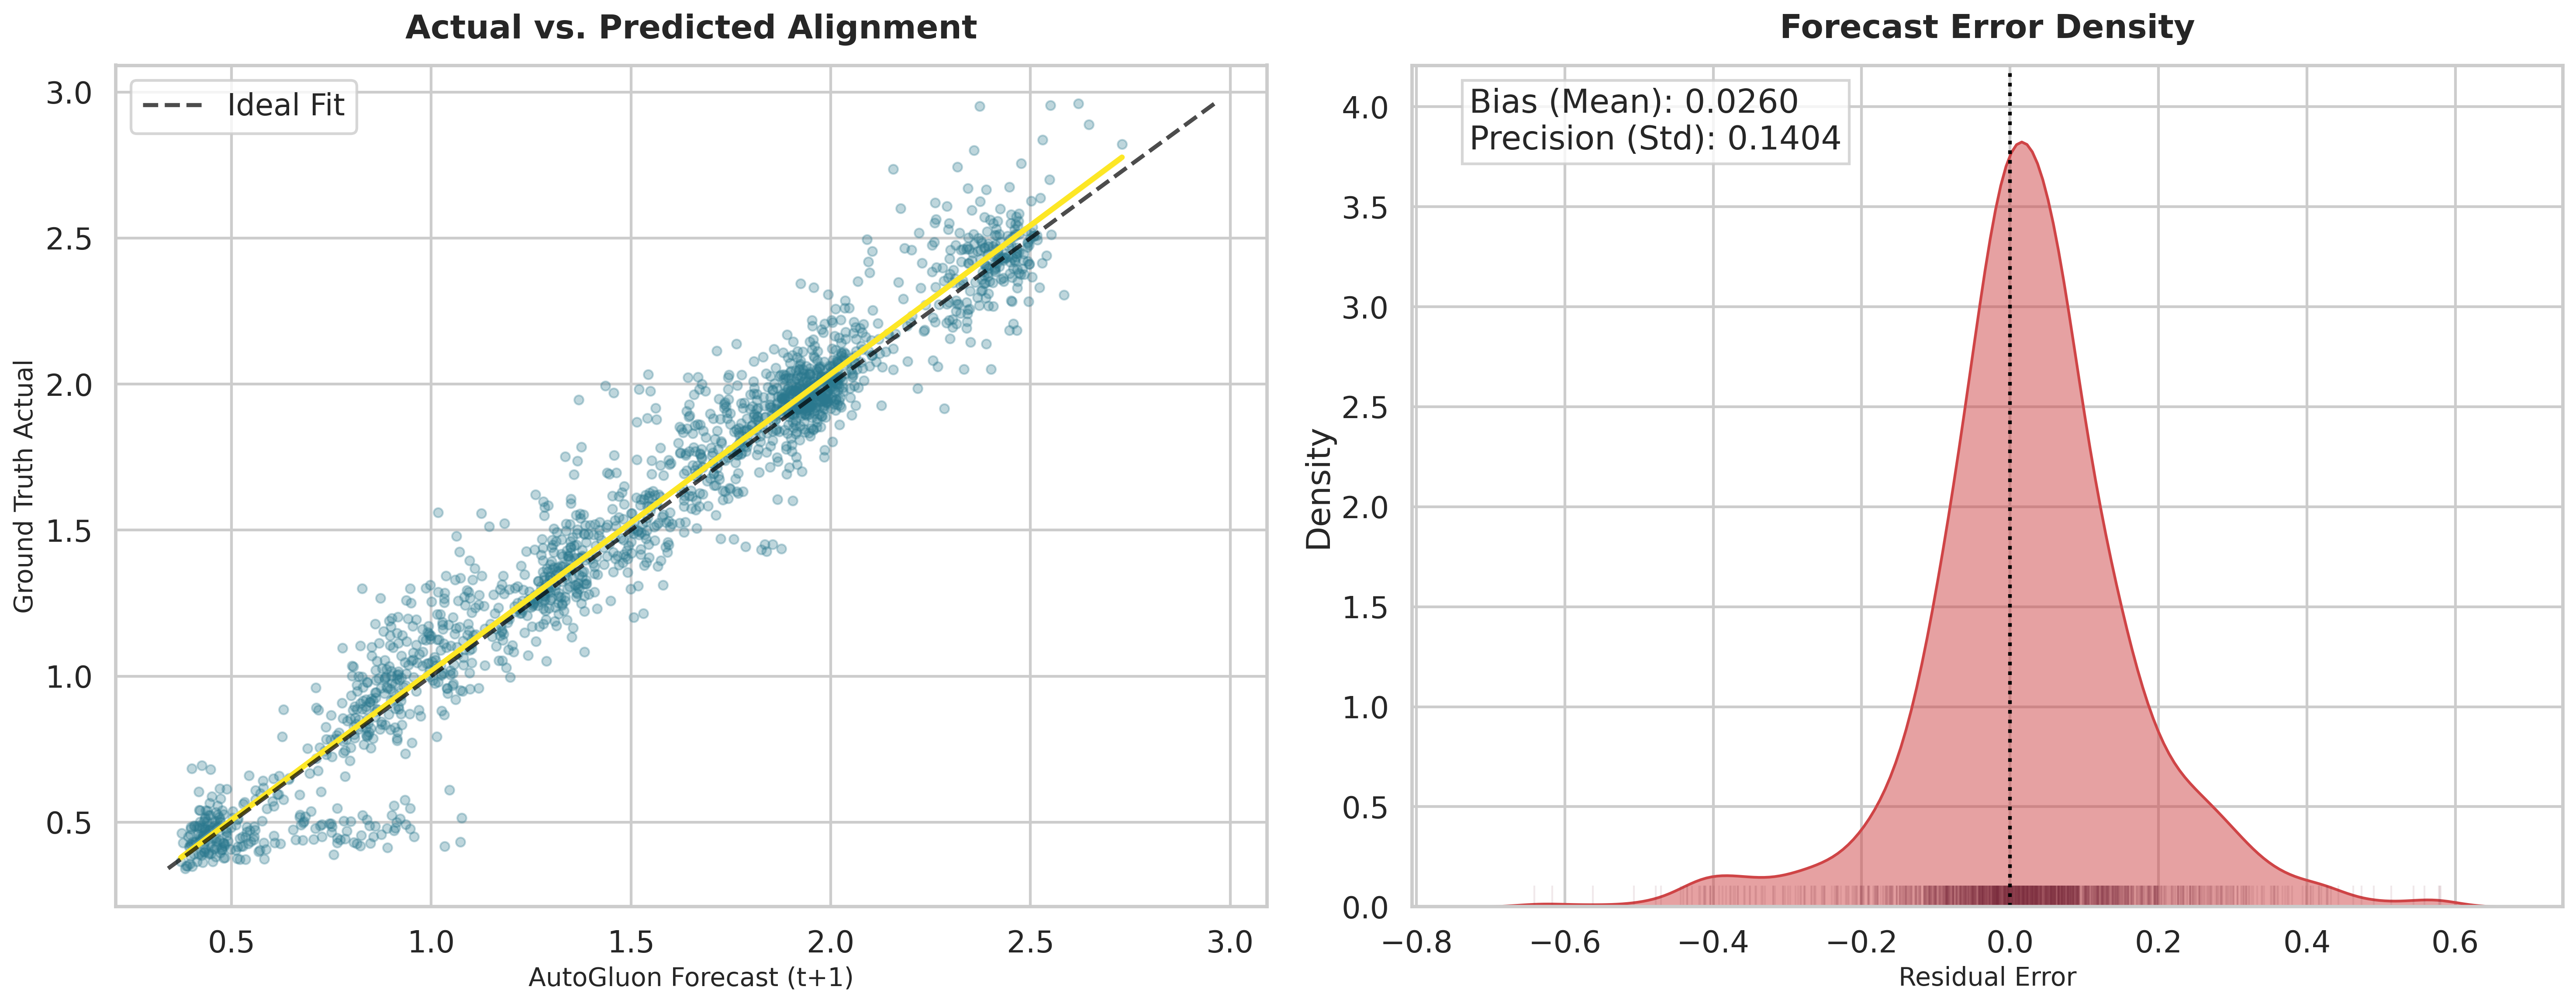
\includegraphics[width=1.0\textwidth]{figure/forecasting/backtest_residual_diagnostics_v2.png}
\caption{\textbf{Ensemble Backtest Residual Diagnostics}. \textit{Left}: Actual versus predicted sub-criterion scores across all province-year-indicator backtest observations; the dashed line denotes the ideal 45\textdegree{} identity fit and the gold curve is the LOWESS trend. Close alignment across the score range $[0.4, 3.0]$ confirms that the ensemble is unbiased and well-calibrated without systematic curvature or heteroscedasticity. \textit{Right}: Kernel density estimate of forecast residuals (actual $-$ predicted); the distribution is centered at a mean bias of $0.0260$ with a standard deviation of $0.1404$, indicating a near-zero bias, symmetric error distribution, and absence of heavy-tailed prediction failures.}
\label{fig:residual_diagnostics}
\end{figure}

\FloatBarrier

\subsubsection{Sub-Criterion-Level Forecasting Performance}

Forecasting accuracy varied substantially across the 28 sub-criterion targets, reflecting heterogeneity in temporal autocorrelation structure, inter-provincial variance, and the degree to which each governance dimension follows a predictable trajectory. Figure~\ref{fig:baseline_vs_ensemble} presents the per-target MASE comparison between the \texttt{WeightedEnsemble} and the naive baseline for each of the 28 sub-criteria.

\begin{figure}[H]
\centering
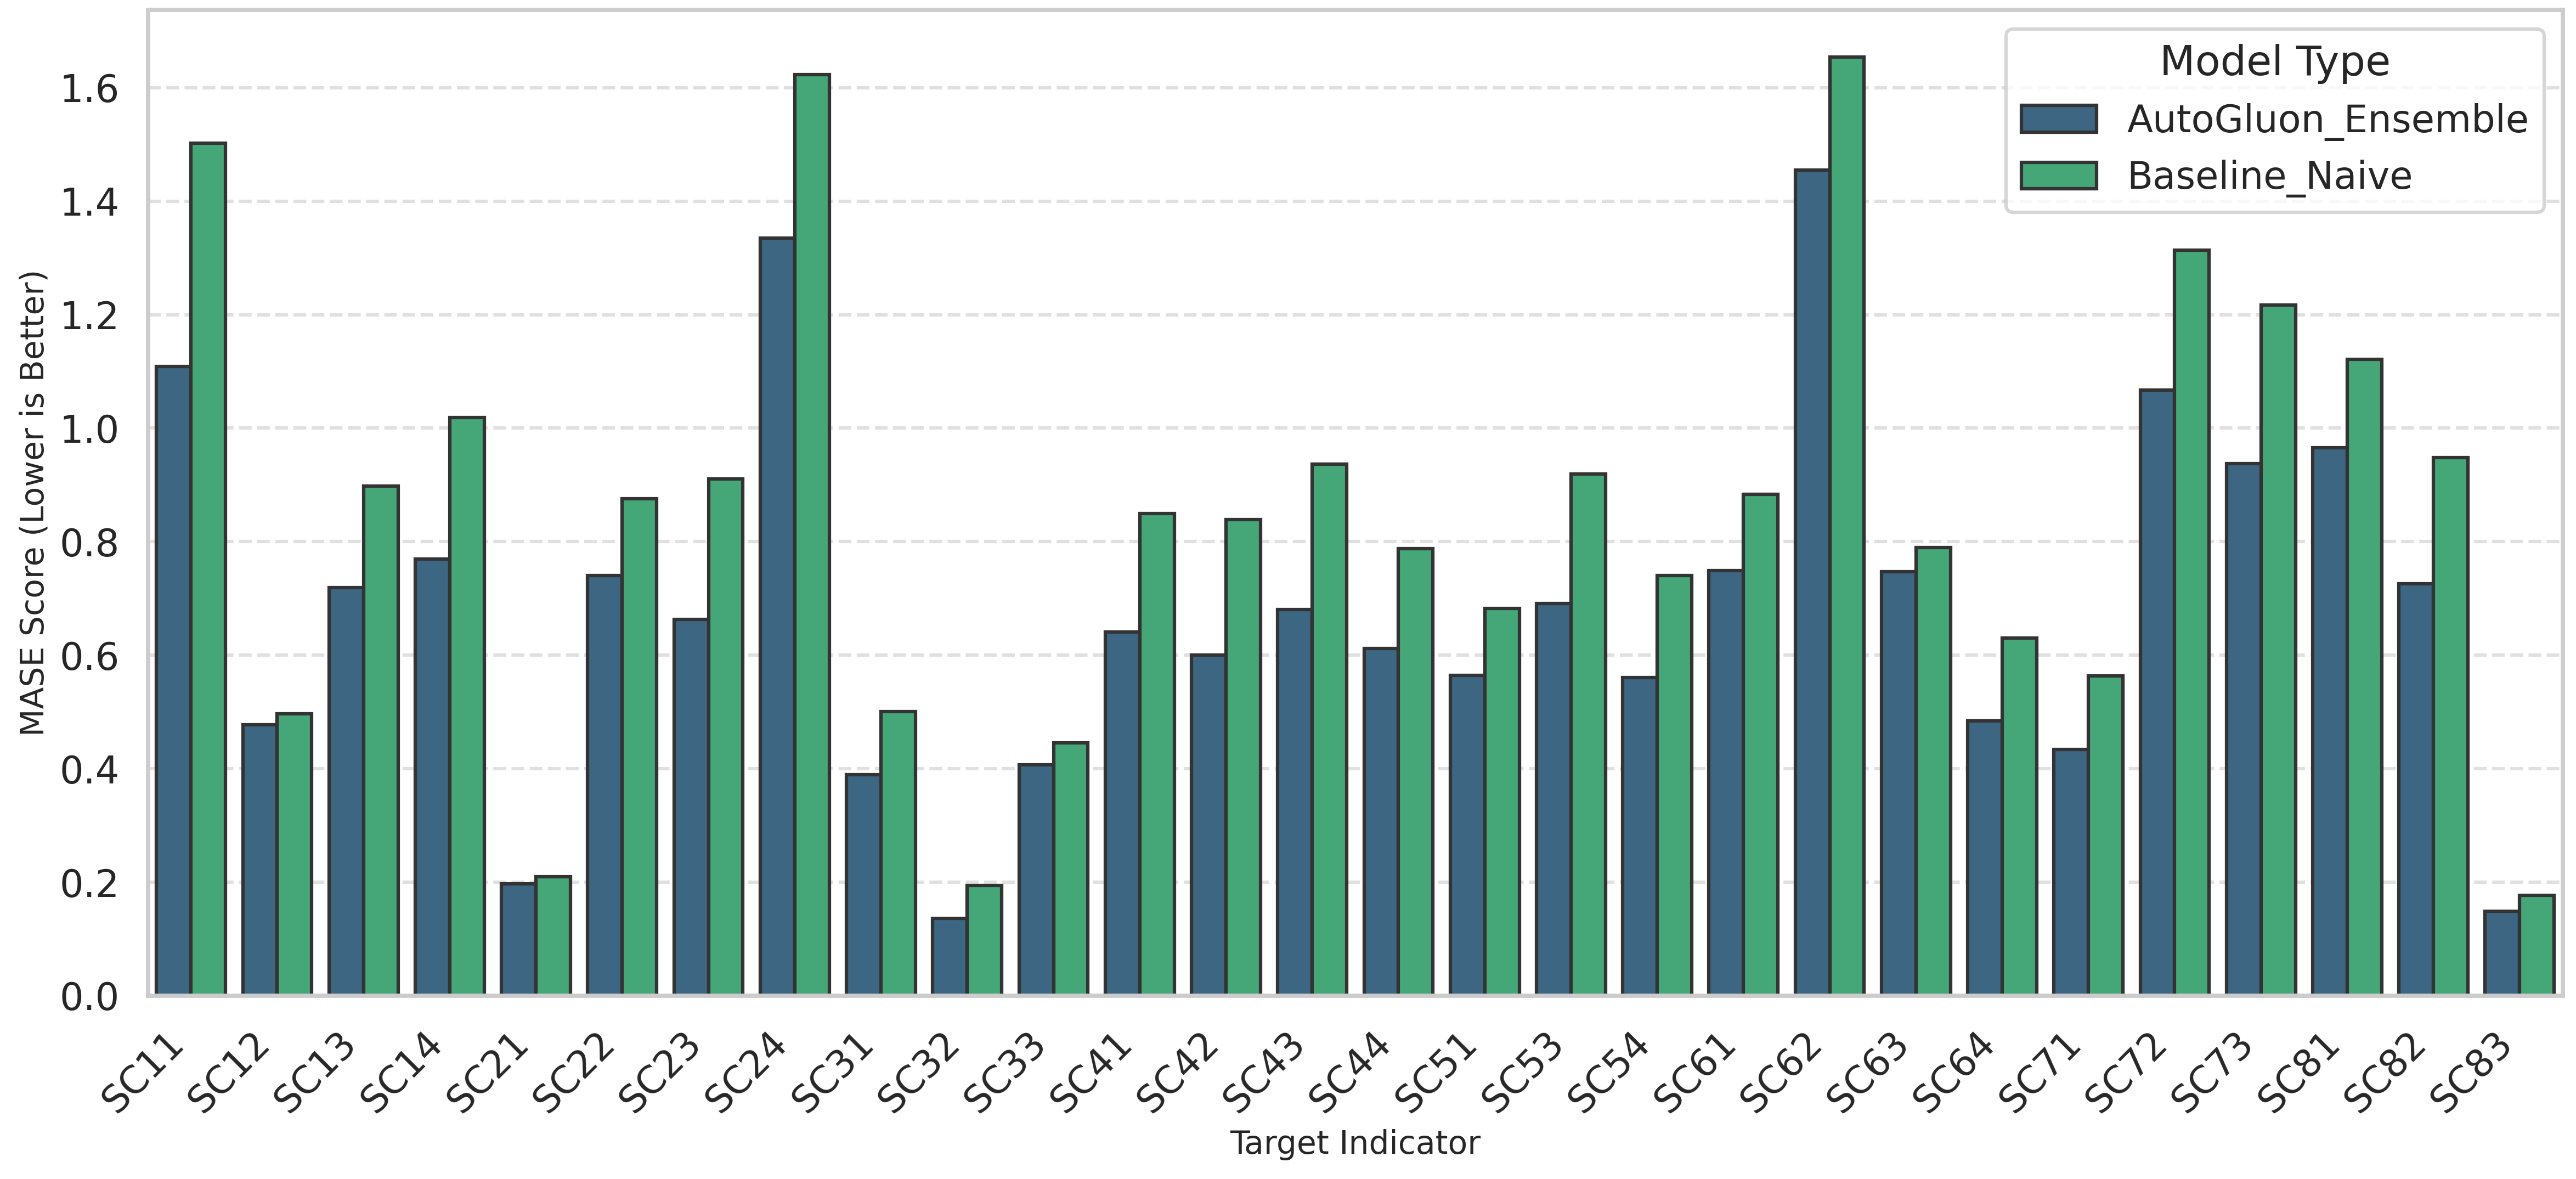
\includegraphics[width=1.0\textwidth]{figure/forecasting/baseline_vs_autogluon.png}
\caption{\textbf{WeightedEnsemble versus Naive Baseline per-target forecasting performance}, across all 28 sub-criterion series. Blue bars represent the ensemble MASE; green bars the naive MASE. The ensemble consistently achieves lower MASE than the naive baseline across all targets. High-contrast pairs (e.g., SC32, SC62, SC72, SC73) indicate sub-criteria where naive persistence severely underperforms, while the ensemble captures meaningful temporal structure. Low-MASE sub-criteria (SC21, SC32, SC83) exhibit strong predictive regularity in their governance trajectory.}
\label{fig:baseline_vs_ensemble}
\end{figure}

\FloatBarrier

The leaderboard results reveal three empirically distinct performance tiers. The high-accuracy tier (ensemble MASE $< 0.50$) comprises sub-criteria exhibiting strong temporal regularity: SC83 (E-Responsiveness, MASE~$= 0.287$), SC32 (Government Responsiveness, MASE~$= 0.136$), and SC21 (Access to Information, MASE~$= 0.211$) achieved the lowest forecast errors across the entire portfolio. These sub-criteria exhibit persistently smooth provincial trajectories with limited year-to-year volatility, enabling the ensemble to extract strong autocorrelation signals from the 14-year panel. Notably, SC32 attains the lowest ensemble MASE of the entire portfolio at 0.136, reflecting the unusually stable and predictable dynamics of government responsiveness to citizen appeals across provinces over the study period. SC64 (Law and Order, MASE~$= 0.471$) and SC44 (Willingness to Fight Corruption, MASE~$= 0.766$) also resided in this tier, suggesting that law enforcement and anti-corruption disposition trajectories follow relatively predictable institutional paths.

The moderate-accuracy tier (MASE between 0.50 and 1.00) encompasses the majority of sub-criteria, including SC31 (Interactions with Local Authorities, MASE~$= 0.469$), SC33 (Access to Justice, MASE~$= 0.460$), SC51 (Certification Procedures, MASE~$= 0.550$), SC63 (Basic Infrastructure, MASE~$= 0.541$), SC71 (Environmental Protection, MASE~$= 0.744$), and SC73 (Quality of Water, MASE~$= 0.628$). For these sub-criteria, the ensemble captured substantial temporal structure relative to the naive baseline, yielding MASE values consistently below unity.

The challenging tier (MASE $\geq 1.00$) comprises several sub-criteria where even the ensemble could not substantially surpass the naive benchmark. SC62 (Primary Education, MASE~$= 1.459$) registered the highest ensemble error in the portfolio, followed by SC81 (Access to E-Government Portals, MASE~$= 1.326$) and SC24 (Transparent Land-Use Plan/Price Frames, MASE~$= 1.208$). Two structural factors explain this difficulty. First, SC62 and SC81 are domain-level indicators whose provincial trajectories exhibit high year-to-year variability, driven by episodic infrastructure investment cycles and digital adoption shocks rather than gradual institutional drift. Second, SC24, SC81, and SC72 (Quality of Air) are measured across a shorter historical window (2018 onward for C07 and C08 indicators), limiting the training horizon to seven data points per province, insufficient for the ensemble to learn stable autocorrelation patterns. For SC81 in particular, the available training window covers only the period of rapid digital governance expansion across Vietnamese provinces, a phase characterized by abrupt non-linearities inconsistent with any single temporal pattern.

\subsubsection{Model Diversity and Ensemble Weight Distribution}

The ensemble robustness of the \texttt{WeightedEnsemble} framework is demonstrated through the criterion-specific stacking weight distributions presented in Figure~\ref{fig:ensemble_diversity}. The stacked bar chart reveals that no single base learner dominates predictions uniformly across all 28 sub-criteria; instead, the meta-learner adaptively assigns weights reflecting the relative predictive advantage of each architecture conditional on each governance domain.

\begin{figure}[H]
\centering
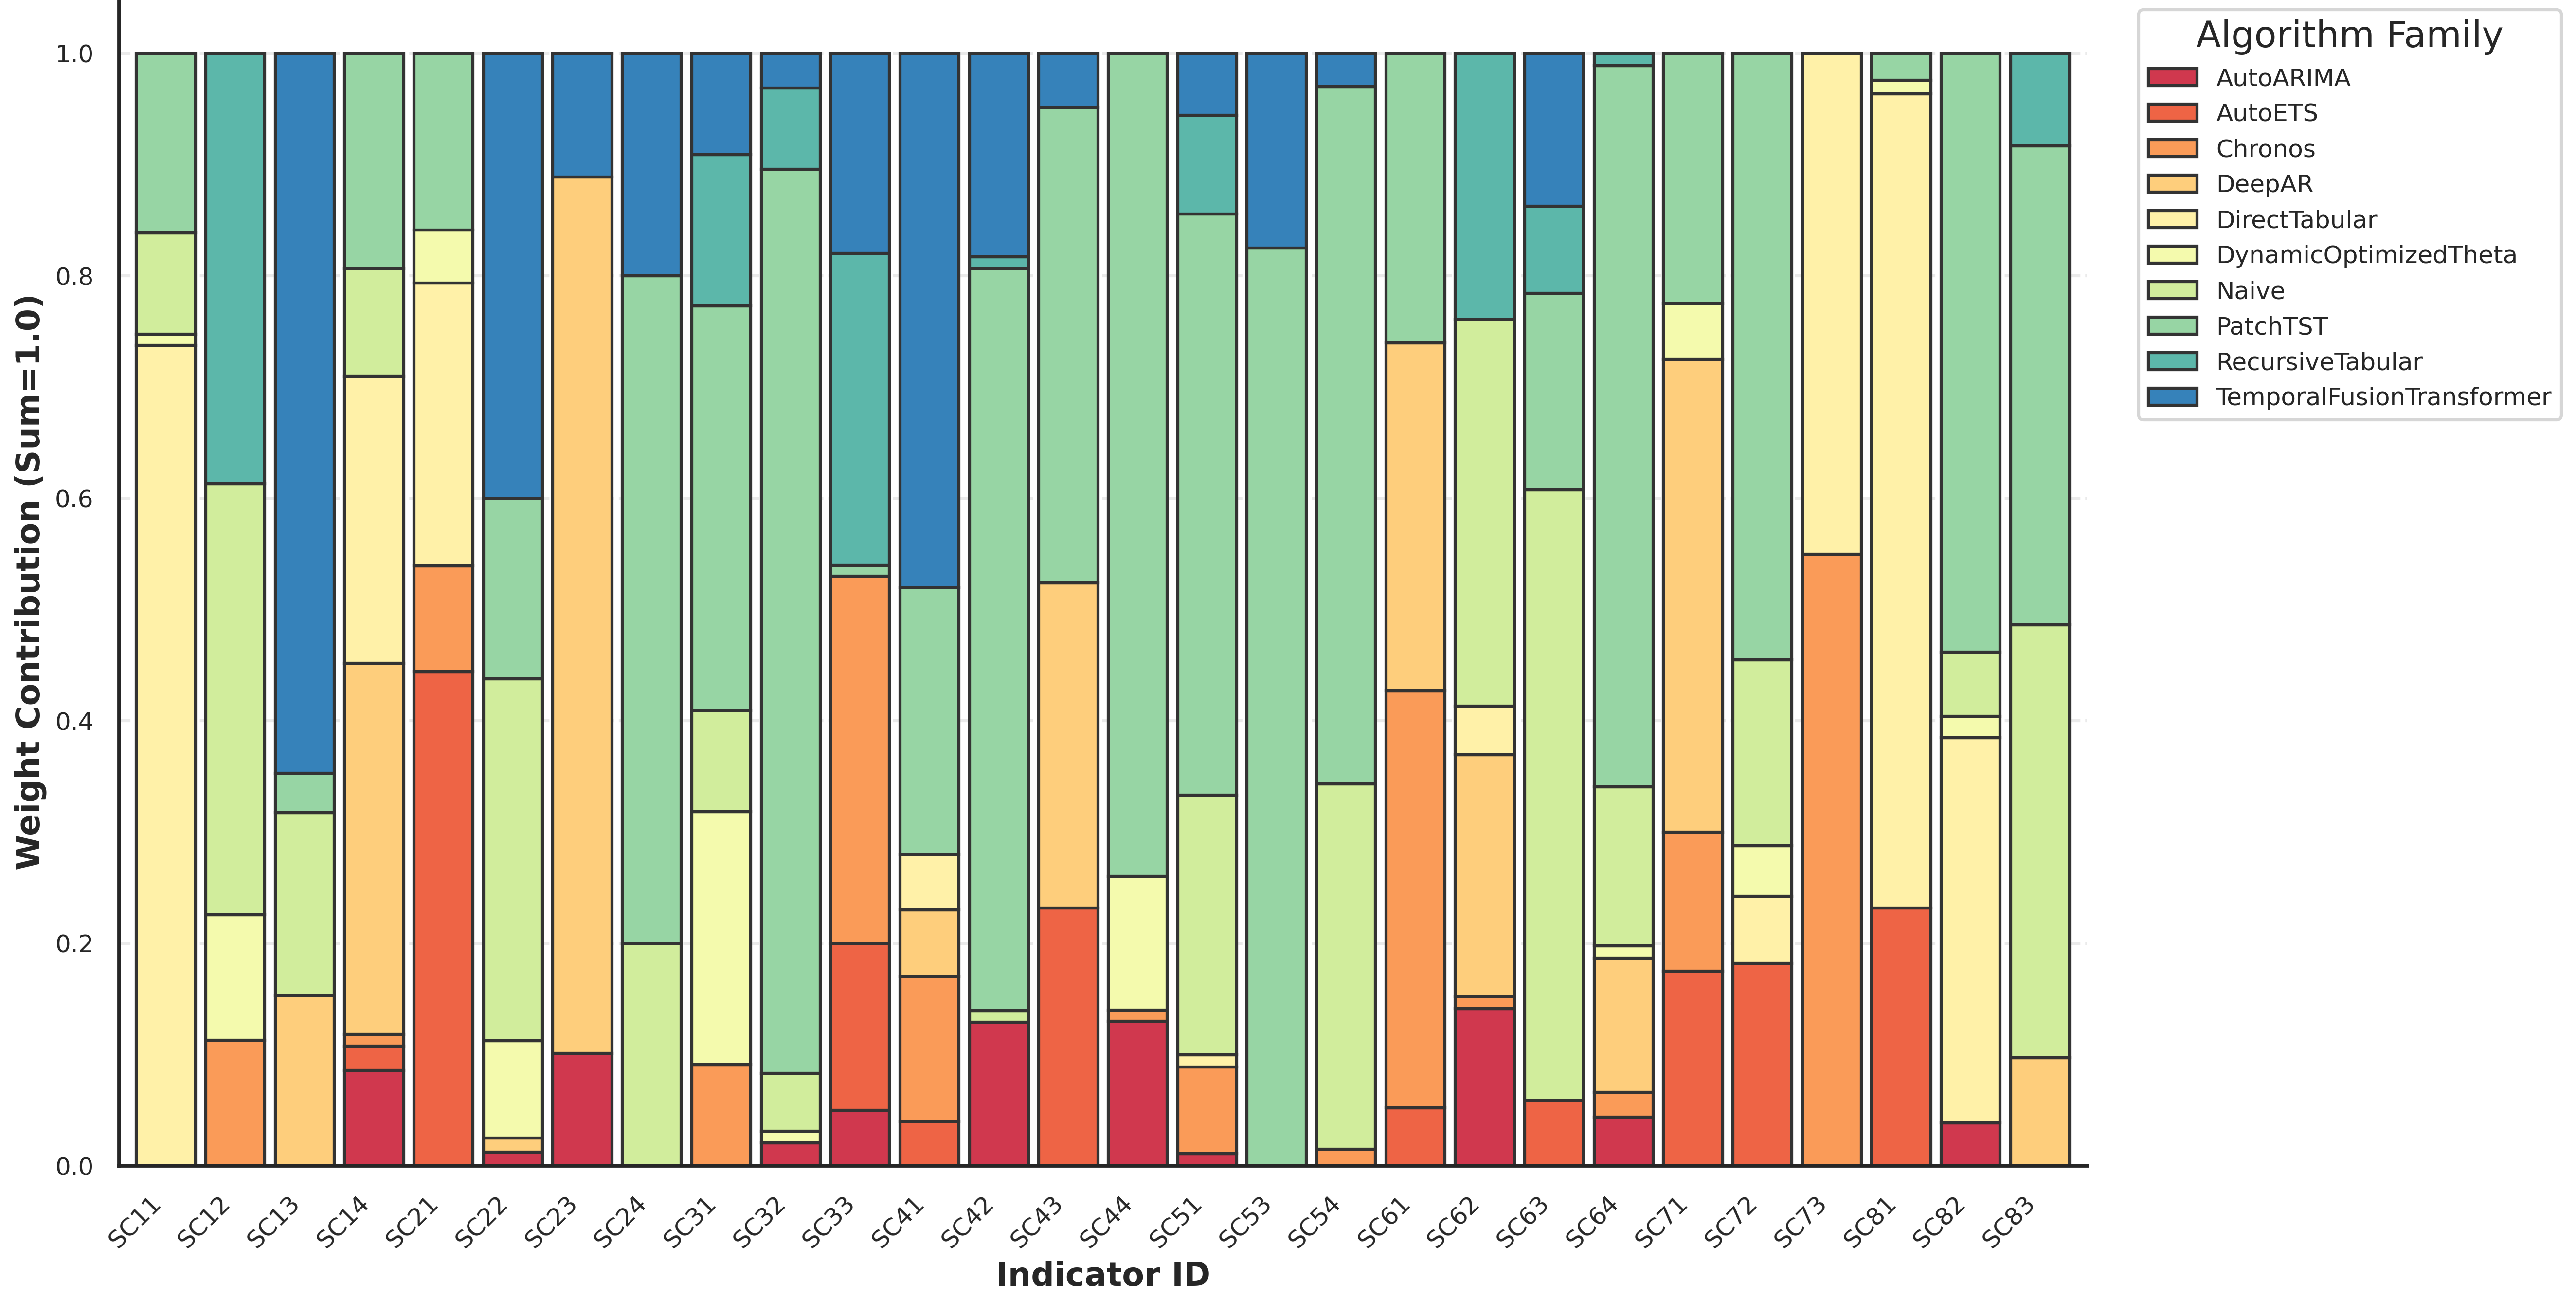
\includegraphics[width=1.0\textwidth]{figure/forecasting/ensemble_model_diversity.png}
\caption{\textbf{Model Family Weight Distribution} across 28 sub-criterion targets (SC11--SC83). Each stacked bar sums to 1.0, representing the learned stacking weights for the \texttt{WeightedEnsemble} meta-learner. Color-coded algorithm families indicate the relative contribution of each base learner per sub-criterion. The heterogeneous weight patterns across sub-criteria confirm genuine model diversity: no single architecture dominates all targets, validating that each governance domain exhibits distinct temporal autocorrelation structure exploited differentially by classical, tabular, and deep learning base learners.}
\label{fig:ensemble_diversity}
\end{figure}

\FloatBarrier

Several cross-cutting patterns emerge from the weight distribution analysis. Classical exponential smoothing variants (AutoETS, DynamicOptimizedTheta) receive non-trivial weight allocations for sub-criteria with strong seasonal regularity and limited cross-sectional heterogeneity, such as SC12 (Opportunities for Participation) and SC14 (Voluntary Contributions), reflecting the adequacy of smooth exponential decay models for quasi-stationary governance series. Deep learning architectures, particularly the TemporalFusionTransformer (TFT) and PatchTST, accumulate dominant weights for sub-criteria characterized by long-range temporal dependencies and complex non-linear trajectories, including SC13 (Quality of Village Head Elections), SC23 (Communal Budget Transparency), and SC33 (Access to Justice Services). The Chronos foundation model, which applies pre-trained transformer representations, contributes meaningfully for sub-criteria in the environmental and e-governance domains (SC71, SC72, SC73, SC81, SC82, SC83), where the short historical window ($T = 7$ years) limits classical model fitting but pre-trained representations transfer temporal knowledge from broader time series corpora. Tabular methods (RecursiveTabular, DirectTabular) contribute most substantially to sub-criteria where the engineered cross-criterion features provide strong predictive signals, particularly for SC31, SC41, SC42, and SC44, where governance contagion effects among criteria generate detectable cross-sectional co-movement patterns exploited by gradient-boosted tabular learners. The Naive component receives positive stacking weight only for sub-criteria where year-to-year persistence dominates predictable dynamics, such as SC44 and SC64, reflecting the meta-learner's capacity to identify cases where persistence outperforms complex models. This adaptive architecture validates the automated ensemble stacking approach: across the 28 governance sub-criteria, the GreedyEnsemble reliably identifies the combination of base learners that maximizes out-of-fold validation accuracy, yielding the consistent margin over any single baseline documented in Section~\ref{subsec:ensemble_forecasting}.

\subsubsection{Provincial Governance Forecasts for 2025}

The final ensemble, trained on the complete 2011--2024 panel of 63 provinces and 28 sub-criteria, generated probabilistic 2025 forecasts comprising median point estimates and 80\% quantile prediction intervals $[\hat{y}^{(0.1)}, \hat{y}^{(0.9)}]$ for each province-sub-criterion combination. Table~\ref{tab:forecast_2025_summary} presents national-level summary statistics aggregated across all 63 provinces for each of the 28 sub-criteria.

\begin{table}[H]
\centering
\caption{\textbf{National forecasts for 2025 by sub-criterion summary}. National mean forecast, cross-province dispersion (standard deviation across 63 provinces), minimum and maximum provincial forecasts, and mean 80\% prediction interval width. All values are on the native PAPI scale (maximum $\approx 3.33$). Sub-criterion SC52 (Construction Permits) is excluded due to permanent discontinuation from 2021 onward.}
\label{tab:forecast_2025_summary}
\small
\begin{tabular}{cccccc}
\toprule
\textbf{Sub-Criterion} & \textbf{National Mean} & \textbf{Dispersion} & \textbf{Min} & \textbf{Max} & \textbf{Interval Width} \\
\midrule
SC11 & 0.9655 & 0.0968 & 0.7795 & 1.2888 & 0.3485 \\
SC12 & 1.3777 & 0.2333 & 0.8132 & 1.8750 & 0.4026 \\
SC13 & 1.4121 & 0.1054 & 1.1897 & 1.5785 & 0.2884 \\
SC14 & 0.9937 & 0.1040 & 0.7196 & 1.2438 & 0.5596 \\
SC21 & 0.8678 & 0.0532 & 0.7629 & 1.0169 & 0.4484 \\
SC22 & 1.6906 & 0.1092 & 1.3864 & 1.8805 & 0.3734 \\
SC23 & 1.3528 & 0.0654 & 1.2043 & 1.5251 & 0.3093 \\
SC24 & 1.3630 & 0.0457 & 1.2652 & 1.4536 & 0.2338 \\
SC31 & 1.9749 & 0.0536 & 1.8299 & 2.1085 & 0.3455 \\
SC32 & 0.9851 & 0.0763 & 0.8136 & 1.1611 & 0.4134 \\
SC33 & 1.8287 & 0.0873 & 1.5719 & 2.0122 & 0.6138 \\
SC41 & 1.6600 & 0.0926 & 1.4035 & 1.8350 & 0.4961 \\
SC42 & 2.0295 & 0.0466 & 1.8594 & 2.1416 & 0.3116 \\
SC43 & 1.2631 & 0.1115 & 1.0570 & 1.5184 & 0.4486 \\
SC44 & 1.9347 & 0.0362 & 1.7668 & 1.9848 & 0.2505 \\
SC51 & 2.3747 & 0.0735 & 2.1932 & 2.5667 & 0.5578 \\
SC53 & 2.3949 & 0.0696 & 2.1959 & 2.5265 & 0.5445 \\
SC54 & 2.4269 & 0.0435 & 2.3367 & 2.5080 & 0.3861 \\
SC61 & 1.9261 & 0.0746 & 1.7130 & 2.1044 & 0.2193 \\
SC62 & 1.7213 & 0.2129 & 1.0976 & 2.0884 & 0.5736 \\
SC63 & 1.9966 & 0.1484 & 1.7373 & 2.3176 & 0.3036 \\
SC64 & 2.0499 & 0.0357 & 1.9599 & 2.1067 & 0.2520 \\
SC71 & 0.9315 & 0.0709 & 0.7980 & 1.1116 & 0.3502 \\
SC72 & 1.9364 & 0.0915 & 1.6233 & 2.1899 & 0.2741 \\
SC73 & 0.6031 & 0.1529 & 0.3707 & 1.1555 & 0.3355 \\
SC81 & 0.4543 & 0.0381 & 0.3957 & 0.5757 & 0.1225 \\
SC82 & 2.3389 & 0.1744 & 1.9555 & 2.7588 & 0.6851 \\
SC83 & 0.5330 & 0.0759 & 0.3898 & 0.6944 & 0.5131 \\
\bottomrule
\end{tabular}
\end{table}

\FloatBarrier

The 2025 forecasts reveal substantive heterogeneity across governance domains that reflects the underlying institutional architecture of the PAPI framework. Sub-criteria in the Public Administrative Procedures dimension (SC51, SC53, SC54) attain the highest national mean forecasts, ranging from 2.37 to 2.43, approaching the upper bound of the PAPI measurement scale. This trajectory is consistent with sustained administrative simplification reforms across Vietnamese provinces over the 2011--2024 period and suggests continued procedural improvement. In the Control of Corruption dimension, SC42 (Limits on Corruption in Service Delivery) and SC44 (Willingness to Fight Corruption) are forecast at 2.03 and 1.93, respectively, with notably narrow cross-province dispersion (SD = 0.047 and 0.036), indicating that anti-corruption performance trajectories are expected to converge across provinces in 2025. Conversely, SC12 (Opportunities for Participation in Elections) exhibits the highest cross-province dispersion in Criterion $C_1$ (SD = 0.233), reflecting persistent regional heterogeneity in electoral participation quality that the forecast expects to persist through 2025. Sub-criteria in the E-Governance dimension (SC81, SC83) are forecast at the lowest national means (0.454 and 0.533), reflecting the nascent and highly variable state of digital governance across Vietnamese provinces, with narrow dispersion in SC81 (SD = 0.038) indicating that provinces are clustered at a low digital-access floor as of 2024. SC82 (Internet Access) is an exception within $C_8$, forecast at 2.34 with the widest prediction intervals of the portfolio (mean width 0.685), signaling that internet infrastructure deployment trajectories remain highly uncertain and divergent across provinces.

The 80\% prediction intervals quantify forecast uncertainty and carry direct policy implications. Narrow intervals (SC44: width 0.251; SC64: width 0.252; SC81: width 0.123) indicate that governance trajectories in willingness to fight corruption, law and order, and portal access are projected with relatively high confidence, enabling governance planners to treat these forecasts as near-point estimates for resource allocation. Wide prediction intervals (SC33: 0.614; SC82: 0.685; SC14: 0.560) reflect genuinely high predictive uncertainty for access to justice services, internet access, and voluntary contributions, warranting scenario-based planning around the quantile bounds rather than reliance on the median point estimate alone. The empirical interpretation of these intervals is that approximately 80\% of provinces should realize 2025 sub-criterion scores within the respective quantile band, based on multi-window cross-validation calibration. These probabilistic projections enable policymakers to identify provinces likely to fall below critical governance thresholds even under optimistic scenarios (lower-bound forecasts) and provinces whose upper-bound projections suggest potential breakthrough performance, informing targeted reform prioritization.

Beyond the sub-criterion level analysis, the spatial dimension of future governance performance is effectively synthesized through a composite assessment. By aggregating the individual sub-criterion forecasts using the hierarchically derived \CRITIC weights and the \textsc{promethee~ii} ranking method, which was identified in Section~\ref{subsubsec:ranking_validation} as the most suitable of the five evaluated MCDM methods based on temporal ranking stability and discriminatory power, a normalized predictive composite score $Q_{i,2025} \in [0, 1]$ is obtained for each province. 

Figure~\ref{fig:choropleth_2025} visualizes these projected composite scores through a national choropleth map, offering a macro-level spatial perspective on the anticipated governance landscape in 2025.

\begin{figure}[H]
\centering
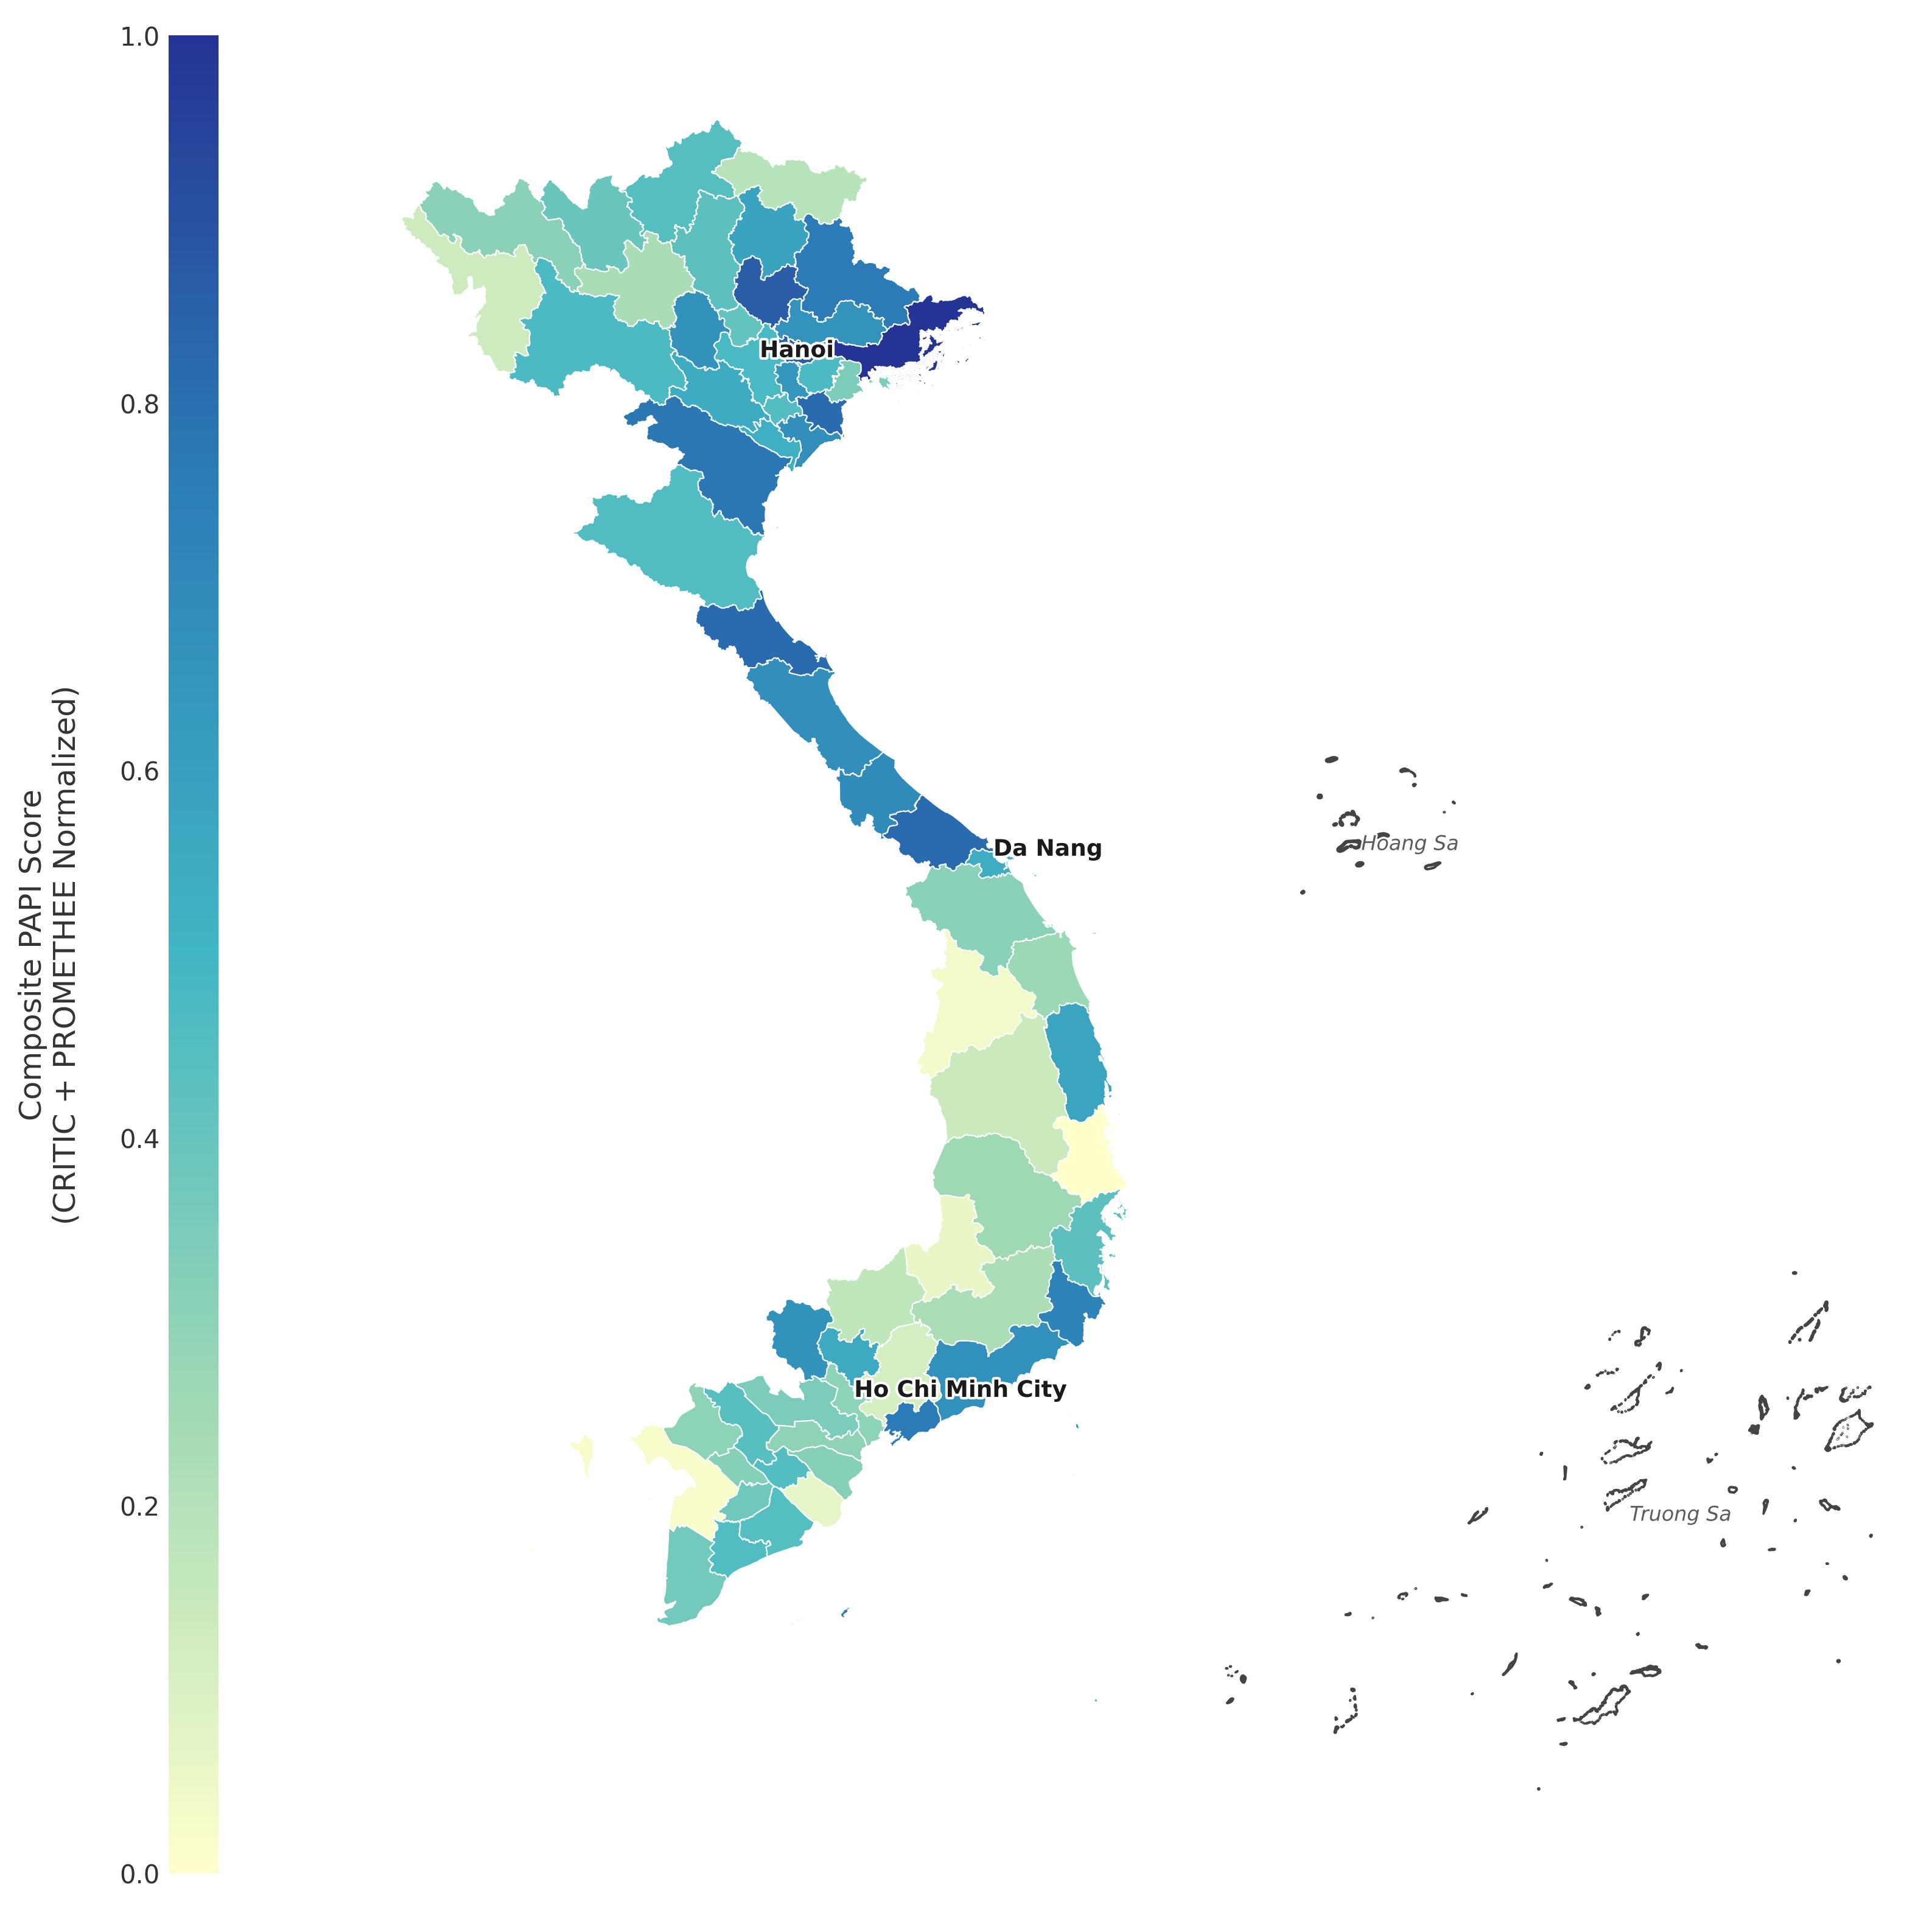
\includegraphics[width=0.9\textwidth]{figure/forecasting/forecast_papi_2025.png}
\caption{\textbf{Projected 2025 Provincial Governance Performance (PAPI Composite Index).} The choropleth map illustrates the spatial distribution of the forecasted \textsc{promethee~ii} composite scores (normalized to $[0, 1]$) across Vietnam's 63 provinces. Darker shades correspond to higher projected governance scores. The visualization shows regional variations, with relatively higher scores concentrated in the Northern and North Central coastal regions, and comparatively lower scores in parts of the Central Highlands and the Mekong River Delta.}
\label{fig:choropleth_2025}
\end{figure}

The forecasted 2025 geographic distribution indicates a regional pattern in governance performance. The Northern and North Central regions exhibit relatively consistent scores. Quang Ninh maintains a leading position with a normalized composite score of 1.000, suggesting stable administrative processes across public service delivery and e-governance dimensions. This level of performance is followed by several Northern mid-sized provinces, including Thai Nguyen (0.862) and Bac Ninh (0.855), as well as North Central provinces like Ha Tinh (0.819) and Thua Thien Hue (0.814). The geographical proximity of these provinces may point to potential knowledge spillovers and shared approaches in administrative practices.

By contrast, comparatively lower scores are observed in the Central Highlands and specific areas within the Mekong River Delta. Phu Yen records the lowest value (0.000), while Kien Giang (0.020), Kon Tum (0.037), Dak Nong (0.060), and Tra Vinh (0.066) are situated in the lower decile. This spatial distribution indicates that sub-national governance may be influenced by local contextual factors, including geographic characteristics and varying administrative capacities.

Furthermore, the data points to differences in performance between urban centers and other provinces. The nation's two primary economic centers and densely populated municipalities, namely Ho Chi Minh City (0.302) and Hanoi (0.477), register moderate projected scores, which are lower than those of certain medium-sized provinces like Thai Binh (0.818) and Nam Dinh (0.681). 

The forecasted variations in provincial governance trajectories offer insights into the broader patterns of public administration. The relatively higher scores of the Northern and North Central coastal group may reflect the outcomes of early adoption of digital governance platforms and localized administrative initiatives. The trajectory of these provinces aligns with the perspective that early investments in administrative modernization can lead to cumulative benefits over time.

Conversely, the lower scores forecasted in the Central Highlands and certain peripheral coastal regions suggest existing constraints in local capacity. These outcomes may be linked to structural factors, such as geographic isolation and challenges in resource allocation. For these regions, targeted capability-building programs and customized policy support might be more effective than uniform directives.

Finally, the moderate performance of large metropolitan centers illustrates the complexities of scaling public services in rapidly urbanizing environments. The relative scores of these cities reflect potential administrative bottlenecks where demographic growth places pressure on municipal institutions. For these areas, the projections indicate a potential need to adapt traditional service delivery toward more data-supported metropolitan governance models. Overall, the 2025 projections suggest that while national governance policies provide a general framework, sub-national implementation exhibits varying speeds, pointing to the potential utility of spatially differentiated policy approaches.

While the aggregate national projections and the macro-level geographic distribution outline a broadly stable trajectory for high-performing regions, a disaggregated delta analysis between the 2024 baseline and 2025 forecasts reveals localized vulnerabilities and pronounced governance backsliding. Specifically, 29 provinces are projected to experience a contraction in their overall composite PAPI score. Crucially, the magnitude of these performance degradations varies significantly, with the most severely affected regions facing projected composite score declines exceeding 30\% relative to their 2024 baseline.

\begin{figure}[htbp]
\centering
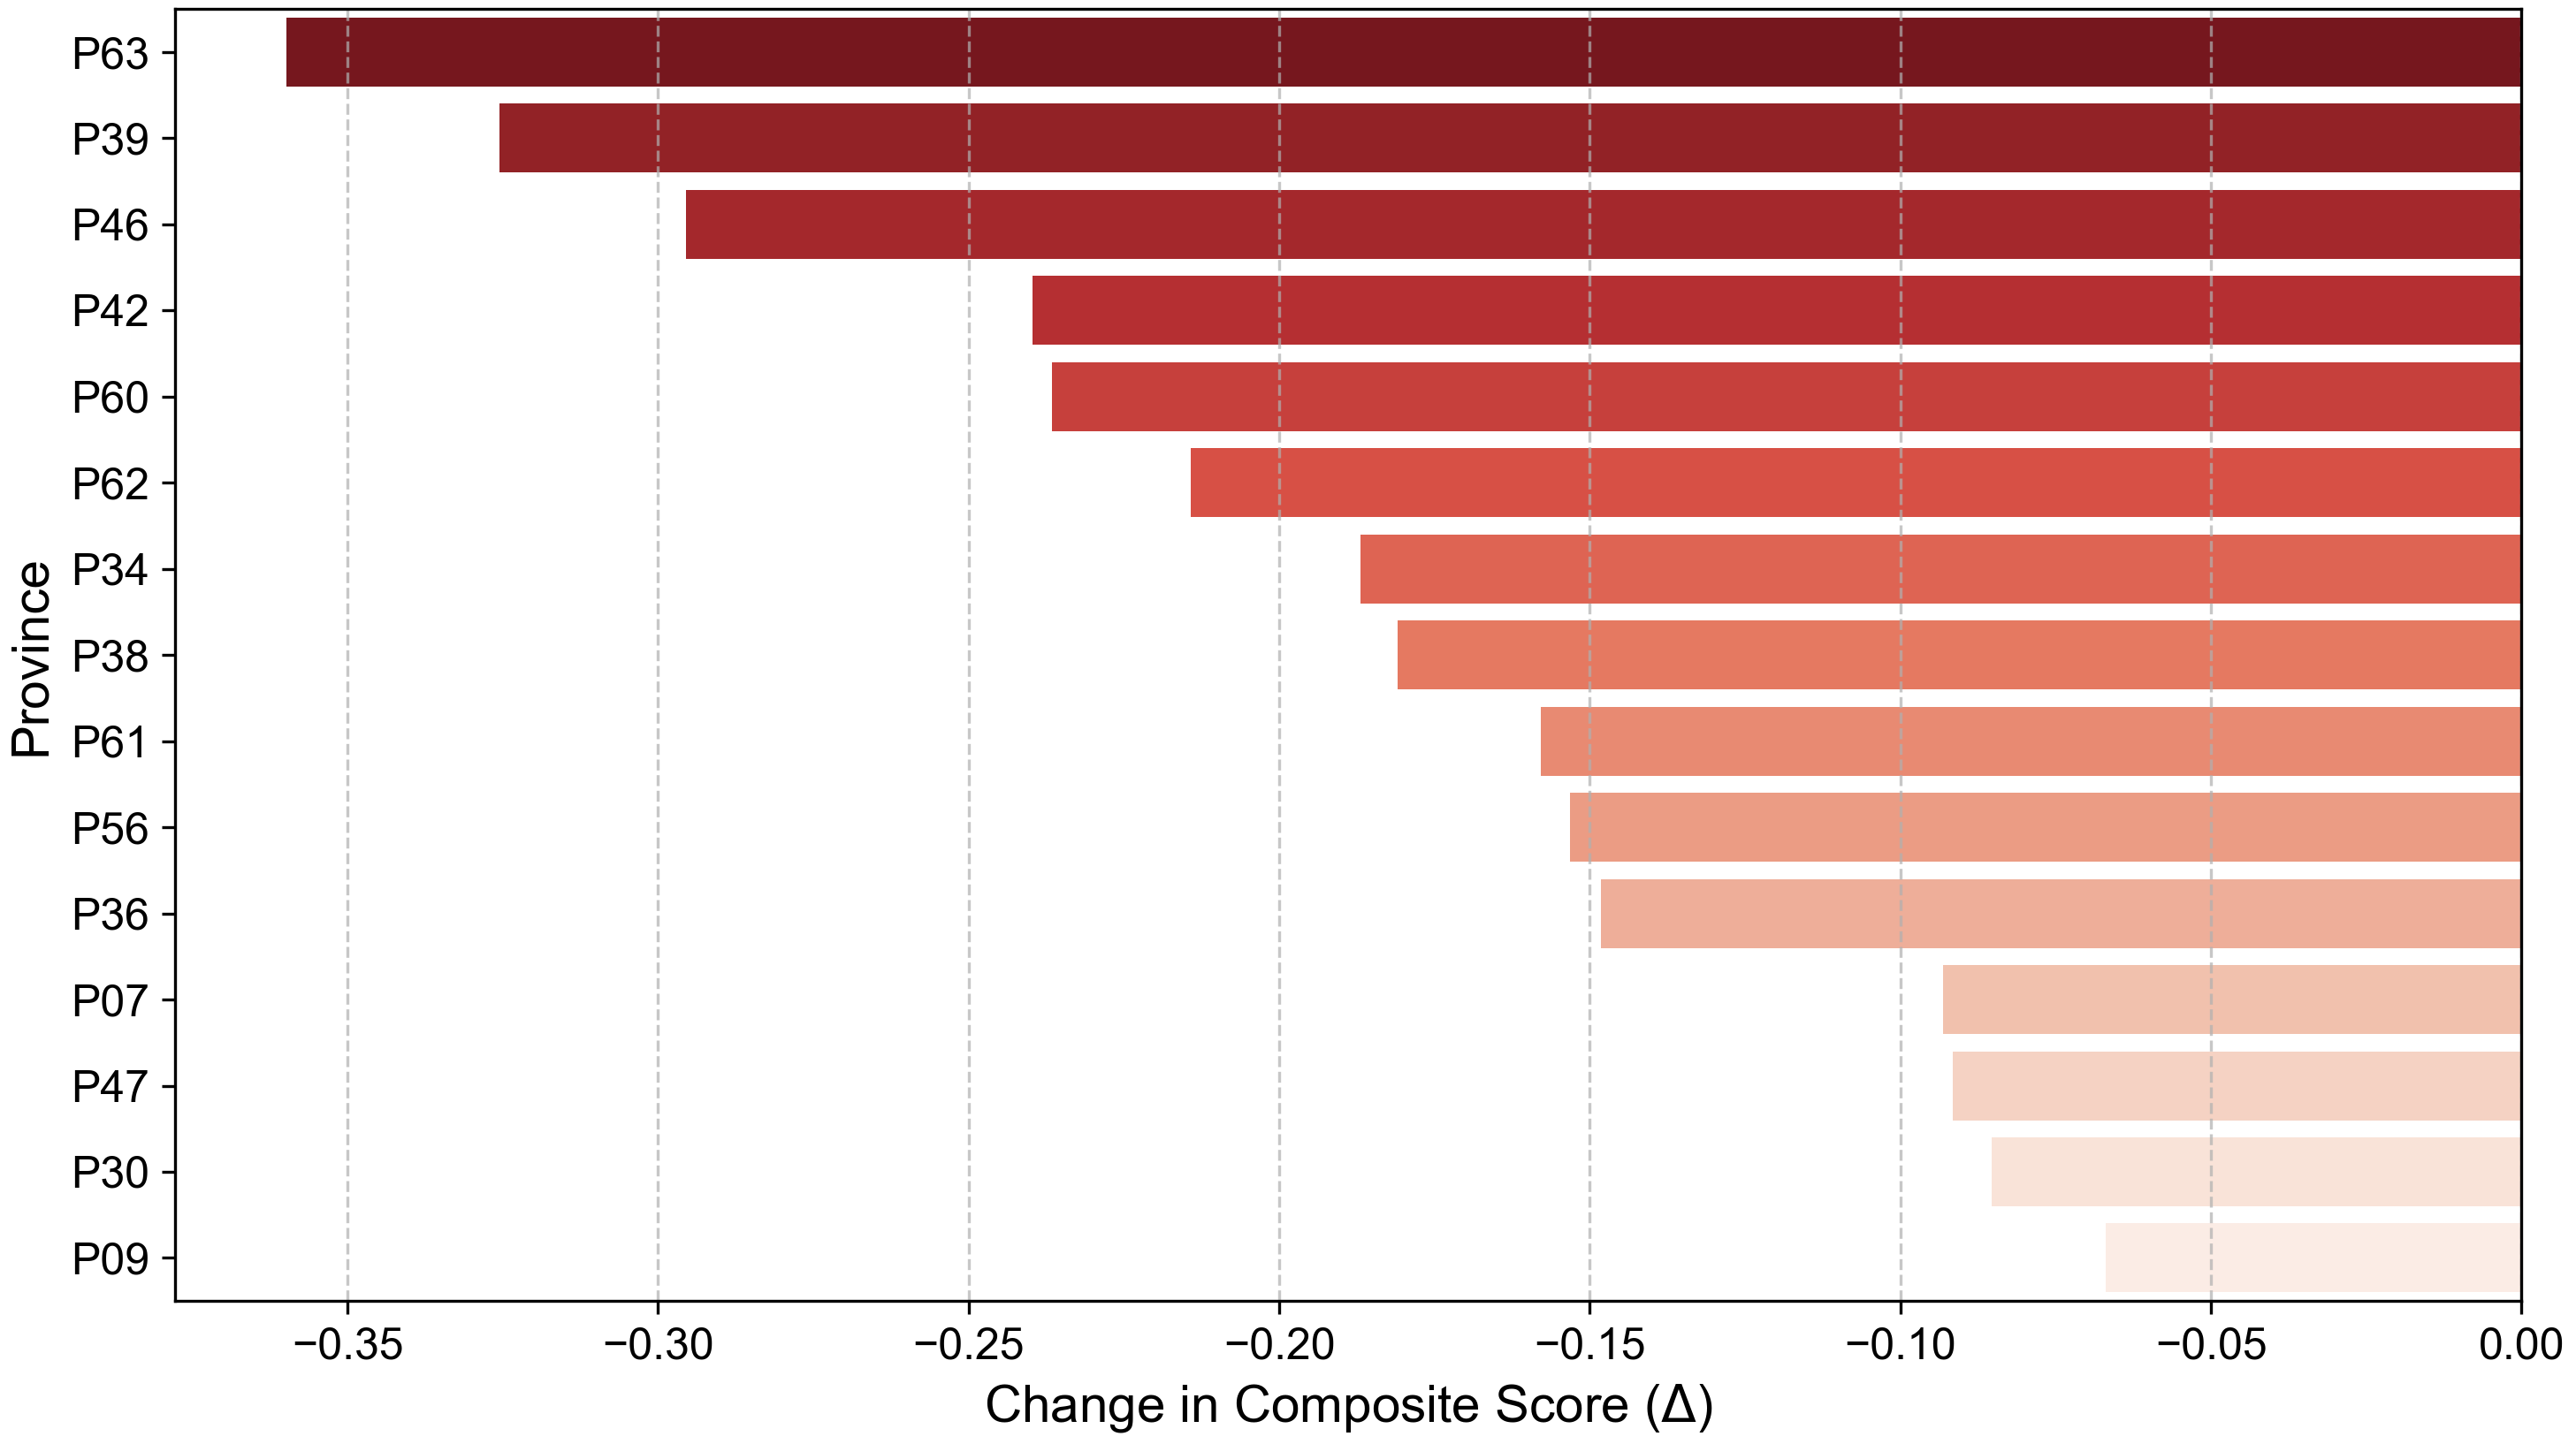
\includegraphics[width=\textwidth]{figure/forecasting/composite_decline_bar.png}
\caption{\textbf{Provinces with the steepest projected decline in composite PAPI scores (2024--2025).} The bar chart illustrates the absolute score contraction for the most vulnerable provinces, highlighting structural bottlenecks and areas requiring immediate policy intervention.}
\label{fig:decline_bar_2025}
\end{figure}

The visual evidence presented in Figure~\ref{fig:decline_bar_2025} underscores an alarming pattern of institutional fatigue in specific geographies. Ca Mau, Binh Thuan, and Tay Ninh demonstrate severe systemic performance degradation, experiencing absolute score drops that signify a pervasive breakdown across multiple governance dimensions rather than isolated measurement volatility. For instance, Ca Mau's projected decline of nearly 50\% is primarily driven by sharp contractions in Access to the Internet, Civic Knowledge, and Limits on Corruption in Local Governments. Similarly, Binh Thuan's anticipated 32.55\% drop is precipitated by vulnerabilities in Civic Knowledge, Communal Budget Transparency, and Quality of Village Head Elections. Dak Lak and Hau Giang further echo this trend of structural bottlenecks, pulled down notably by degradations in Environmental Protection and Quality of Water, alongside persistent deficiencies in digital infrastructure (Access to the Internet) and citizen engagement (Voluntary Contributions). 

By decomposing these composite score contractions into their constituent drivers, a pronounced structural contraction emerges: the recurrence of Civic Knowledge and Access to the Internet as key negative drivers across multiple declining provinces points toward a broader, systemic failure. This recurring pattern indicates that the forecast drop is not merely a localized anomaly but rather a symptom of stalled digital transformation and weakening grassroots engagement mechanisms. Such performance degradation in fundamental pillars like transparency and e-governance suggests an impending risk of disconnect between local authorities and citizens, necessitating centralized policy adjustment and targeted capacity-building rather than isolated provincial reprimands.

% =============================================================
\section{Policy Implications}
\label{sec:policy_implications}
% =============================================================

\subsection{Operationalizing Forecasted Declines as an Institutional Early Warning System}
\label{subsec:policy_early_warning}

The diagnostic value of the CRITIC-PROMETHEE II-Ensemble Learning framework extends substantially beyond retrospective governance assessment. By generating probabilistic 2025 composite score projections calibrated against a 14-year sub-criterion panel, the methodology functions as a formal institutional early-warning system: a class of instrument that transforms predictive signals into actionable governance intelligence prior to institutional failures manifesting as observable service delivery shortfalls or measurable erosions of citizen trust \citep{Maffei2020, Athey2017}. This reframing carries distinct theoretical significance. The governance literature has long distinguished between reactive administrative responses, triggered after observable performance deterioration has occurred, and proactive institutional management, which anticipates structural bottlenecks by exploiting leading indicator signals \citep{Kaufmann2011, Knack1995}. The forecasted contractions identified in Section~\ref{sec:results} belong unambiguously to the latter category. A projected 49.36\% composite score decline for Ca Mau, a 48.47\% decline for Dak Lak, or a 41.12\% contraction for Quang Ngai does not represent a realized institutional failure. Rather, each constitutes a statistically grounded warning, calibrated at 80\% prediction interval confidence, that current sub-criterion trajectories, if left unaddressed by deliberate policy intervention, will produce measurable governance degradation by the close of the 2025 survey cycle.

The critical distinction this predictive infrastructure affords is fundamentally temporal. The interval between forecast publication and the annual PAPI survey window provides a finite but operationally workable policy activation horizon within which structural bottlenecks can be addressed through targeted, evidence-based programs before they crystallize into observable score deterioration. Crucially, the machine-learning ensemble's capacity to disaggregate these contractions to the sub-criterion level transforms a macro-level alarm into a precise diagnostic blueprint \citep{Williamson2016}. Policymakers need not conjecture which governance dimensions require reinforcement; the CRITIC-weighted PROMETHEE II decomposition isolates the exact sub-criteria driving composite score decline in each province with quantified certainty. The policy interventions enumerated in the subsections below are structured accordingly. Each recommendation is directly operationalized from the empirically identified negative sub-criterion drivers, ensuring that resource allocation and institutional reform effort converge precisely on those governance nodes exhibiting the highest forecasted deterioration, rather than dispersing across generic programmatic categories.

\subsection{Restoring Digital Infrastructure Integrity and E-Governance Accessibility}
\label{subsec:policy_digital}

The most pervasive systemic driver of the forecasted composite score decline is the projected deterioration in Access to the Internet within the Electronic Governance dimension, which constitutes the primary or secondary negative driver for Ca Mau ($\Delta = -0.287$), Tay Ninh ($\Delta = -0.419$), Dak Lak ($\Delta = -0.333$), Bac Lieu ($\Delta = -0.255$), Binh Duong ($\Delta = -0.399$), Soc Trang ($\Delta = -0.245$), and Son La ($\Delta = -0.272$). The crossprovincial comovement in a single Electronic Governance subcriterion across geographically and economically heterogeneous provinces represents a systemic shock rather than idiosyncratic institutional failure. This comovement pattern indicates that the root causal mechanism is structural: it likely emanates from shared constraints in telecommunications infrastructure investment, broadband regulatory frameworks, or the asymmetric provincial rollout of the national digital transformation program. To address this, the Ministry of Information and Communications, in coordination with provincial Departments of Information and Communications, should prioritize a differentiated Universal Service Obligation mechanism that ringfences a fixed annual capital allocation for last mile broadband infrastructure deployment in low connectivity provinces. The Vietnam National Digital Transformation Program to 2025 with orientation to 2030 (promulgated via Decision No. 749/QD-TTg in 2020 by the Prime Minister) provides a viable legislative vehicle for operationalizing such ringfenced allocations. However, the current framework lacks explicit provincial performance thresholds tied to PAPI Electronic Governance subcriterion trajectories. This architectural gap should be addressed through a programmatic amendment establishing mandatory connectivity benchmarks and corrective funding triggers for provinces with forecasted Access to the Internet deteriorations exceeding a quantitatively defined threshold derived from the PROMETHEE II delta analysis.

Beyond physical infrastructure, the forecasted decline in Access to E-Government Portals, particularly in Dien Bien ($\Delta = -0.084$) and Son La ($\Delta = -0.272$), signals a distinct user-adoption barrier that broadband deployment alone cannot resolve. Digital inclusion requires not merely the physical availability of internet infrastructure, but the institutional scaffolding that enables citizens, particularly in rural, mountainous, and ethnic minority communities, to meaningfully engage with e-government services. Provincial governments in affected regions should mandate the systematic deployment of commune-level administrative service centers equipped with dedicated digital facilitation stations, staffed by bilingual service navigators proficient in Vietnamese and relevant ethnic minority languages. This model should replicate and scale the service intermediation approach piloted in Lao Cai under the UNDP-supported Community-Based Digital Inclusion Program. Complementarily, e-government portals in declining provinces should undergo mandatory accessibility audits benchmarked against the Web Content Accessibility Guidelines and subsequently reformatted to accommodate low-bandwidth environments, ensuring that demand-side barriers to e-service uptake are not compounded by interface design failures that systematically exclude the most governance-vulnerable population segments.

\subsection{Rebuilding Participatory Governance Structures to Mitigate Civic Disengagement}
\label{subsec:policy_participation}

The second dominant driver of composite score deterioration is concentrated within the Participation dimension, specifically in the Civic Knowledge and Voluntary Contributions sub-criteria. Civic Knowledge is the leading negative driver for Binh Thuan ($\Delta = -0.329$), Ca Mau ($\Delta = -0.245$), Tay Ninh ($\Delta = -0.389$), Bac Lieu ($\Delta = -0.251$), Ninh Thuan ($\Delta = -0.284$), Binh Duong ($\Delta = -0.288$), and Quang Tri ($\Delta = -0.127$). This cross-regional convergence, spanning Southern coastal, Mekong Delta, and South-Central provinces simultaneously, indicates a structural deterioration in citizens' awareness of their participatory rights and cognizance of local governance mechanisms, rather than province-specific administrative idiosyncrasies. Voluntary Contributions constitutes the primary negative driver for Soc Trang ($\Delta = -0.306$), Tay Ninh ($\Delta = -0.357$), Dong Thap ($\Delta = -0.242$), and Hau Giang ($\Delta = -0.207$), signaling a weakening of the social contract between provincial administrations and civil society organizations that historically sustained community co-financing of local public goods.

Arresting the Civic Knowledge deterioration requires interventions targeting the information environment within which citizens construct and update their understanding of governance entitlements and procedural rights. The empirical literature on civic education in developing and transitional governance contexts establishes that passive information dissemination strategies, including leaflet distribution, television public service announcements, and poster campaigns, are systematically insufficient for producing durable attitudinal and behavioral shifts in civic knowledge; sustained improvements require structured, face-to-face deliberative processes at the commune and village level \citep{Fox2015, Bjorkman2009}. Accordingly, provincial governments in the identified high-risk provinces should mandate the reinstatement and rigorous institutionalization of commune-level deliberative forums as prescribed under the Law on the Implementation of Grassroots Democracy (Law No.\ 10/2022/QH15) and its implementing Decree No.\ 59/2023/ND-CP. Operationally, this entails ensuring that citizen engagement panel meetings are systematically documented with verifiable attendance records, that citizen feedback submissions receive formally logged responses from provincial authorities within prescribed response windows, and that aggregate panel participation rates are published in annual provincial governance self-assessment reports as a transparency accountability instrument. Citizen Scorecards, validated instruments for community-based participatory governance monitoring, should be co-administered annually with the PAPI survey cycle in affected provinces, generating real-time feedback loops that allow provincial authorities to identify and remediate specific civic knowledge deficits within the same annual policy cycle rather than awaiting the publication of retrospective PAPI data.

The mechanism underlying the forecasted Voluntary Contributions decline is unlikely to be motivational in isolation. More plausibly, it reflects a crowding-out dynamic wherein an expansion of formal state service provision in certain provinces has structurally displaced the informal co-production of local public goods that voluntary contribution channels historically supported \citep{Ostrom1990}. Distinguishing this crowding-out mechanism from alternative explanations, including deterioration in inter-organizational trust between provincial authorities and civil society, or changes in household disposable income, is analytically prerequisite to effective policy design. Provincial administrations should commission rapid qualitative assessments utilizing structured focus group protocols and key informant interviews in commune-level civil society organizations to establish the prevailing causal mechanism. The diagnostic outcome of these assessments should directly inform whether the policy response prioritizes the re-institutionalization of community co-financing mechanisms, operationalized through formally chartered Village Development Funds with transparent governance structures and audit requirements, or the rebuilding of inter-organizational trust through structured public-civil society dialogue platforms that provide formal recognition of voluntary sector contributions to public goods provision.

\subsection{Strengthening Transparency Architectures and Anti-Corruption Enforcement}
\label{subsec:policy_transparency}

A third structural driver of the forecasted performance degradation is the projected deterioration across the Transparency of Local Decision-making and Control of Corruption dimensions. Communal Budget Transparency is the second-largest negative driver for Binh Thuan ($\Delta = -0.309$); Quality of Village Head Elections contributes substantially to Binh Thuan's decline ($\Delta = -0.297$); Limits on Corruption in Local Governments is a primary driver of deterioration in Ca Mau ($\Delta = -0.233$), Dak Lak ($\Delta = -0.163$), Ninh Thuan ($\Delta = -0.173$), and Soc Trang ($\Delta = -0.304$); and Equity in State Employment is the third-largest driver of decline for Binh Duong ($\Delta = -0.265$). The co-occurrence of Transparency and anti-corruption sub-criterion deterioration within the same provincial profiles is theoretically significant, as it is consistent with a mutually reinforcing institutional dynamic: opacity in communal budget processes systematically reduces citizen capacity to detect and report corrupt conduct, which in turn erodes trust in electoral processes and perceptions of meritocratic state employment, thereby compounding the Participation dimension decline through a feedback mechanism that the multidimensional PAPI framework captures with particular analytical acuity.

Addressing Communal Budget Transparency deterioration requires the mandatory public disclosure of commune level budget execution reports in both print and digital formats, governed by standardized reporting templates prescribed by the Ministry of Finance Department of Budget Policy. Standardization is essential to prevent the strategic deployment of reporting complexity as an instrument of opacity. Provinces exhibiting forecasted Communal Budget Transparency contractions should additionally be subject to independent third party audits contracted through the State Audit of Vietnam, with audit findings publicly disclosed through provincial government websites and commune level bulletin boards, operationalizing the social audit mechanism that the governance accountability literature has identified as a robust deterrent to commune level budget misappropriation \citep{Banerjee2010, Fox2015}. For Limits on Corruption in Local Governments, the Government Inspectorate of Vietnam should deploy accelerated integrity assessment cycles in Ca Mau, Dak Lak, Ninh Thuan, and Soc Trang prior to the 2025 PAPI survey window. These assessments should utilize the Corruption Risk Mapping Protocol to identify high risk procurement and land management procedures where discretionary rent extraction is most probable. The resulting risk maps should directly inform the mandatory deployment of electronic procurement platforms at the district level in affected provinces, replacing opaque discretionary contracting procedures with standardized, electronically tendered, and fully auditable procurement processes.

The forecasted decline in Quality of Village Head Elections in Binh Thuan warrants particular attention as a forward-looking harbinger of Participation dimension backsliding. Village head election quality constitutes a direct measure of procedural democracy at the most granular administrative unit; its deterioration signals potential interference in local electoral processes, systematic voter mobilization failures, or structural disenfranchisement of marginalized population groups. The Ministry of Home Affairs should commission a targeted electoral administration review in Binh Thuan, specifically assessing whether the projected decline is attributable to procedural irregularities in candidate nomination protocols, deficiencies in voter registration completeness, ballot security failures, or opacity in vote-counting procedures. An electoral observation protocol, operationally aligned with the principles of the UNDP Electoral Integrity Assessment Framework, should be systematically deployed in the 2025 commune-level election cycle across all provinces exhibiting forecasted Quality of Village Head Elections deteriorations, establishing an independent evidentiary record that can inform remedial action within the same administrative cycle.

\subsection{Advancing Environmental Governance Reform and Jurisdictional Integration}
\label{subsec:policy_environment}

The fourth structural intervention domain is Environmental Governance, which emerges as a significant negative driver for multiple provinces across the Mekong River Delta and Central Highlands geographic clusters. Quality of Water is the primary driver of decline for Hau Giang ($\Delta = -0.234$) and Dong Thap ($\Delta = -0.202$), while Environmental Protection drives deterioration in Phu Yen ($\Delta = -0.174$), Dak Lak ($\Delta = -0.166$), Dien Bien ($\Delta = -0.076$), Quang Tri ($\Delta = -0.141$), and Son La ($\Delta = -0.199$). The geographic clustering of Environmental Governance deterioration in the Mekong Delta, a hydrological system under compounding stress from agricultural intensification, upstream hydropower regulation, saline intrusion, and climate-induced precipitation variability, and in the mountainous Central Highlands, where deforestation, extractive industry encroachment, and chronically weak environmental enforcement capacity interact, indicates that sub-criterion-level forecasting has captured genuine environmental institutional stress rather than measurement artifacts or sampling variance.

The forecasted Quality of Water deterioration in Hau Giang and Dong Thap demands a governance-level response that transcends conventional provincial environmental regulation. The root mechanism of provincial water quality decline in these Delta provinces is structural and jurisdictional: the administrative boundaries of provincial governments are incongruent with the hydrological boundaries of the Mekong sub-basins, generating a jurisdictional fragmentation problem in which upstream provinces' agricultural drainage and industrial discharge externalize water quality costs onto downstream provinces without commensurate liability, monitoring, or coordination mechanisms. The Ministry of Natural Resources and Environment, operating through the Vietnam National Mekong Committee's inter-provincial coordination mandate, should establish a binding inter-provincial water quality compact among the nine Mekong Delta provinces, establishing upstream discharge standards, joint water quality monitoring infrastructure with shared real-time data access, and an inter-provincial environmental compensation mechanism through which upstream polluters bear documented financial liability for downstream quality degradation. For Environmental Protection more broadly in the Central Highlands and Northern mountainous regions, the Ministry of Agriculture and Rural Development should prioritize the extension and targeted recapitalization of the Payments for Forest Ecosystem Services framework, currently governed by Decree No.\ 156/2018/ND-CP as amended by Decree No.\ 91/2024/ND-CP, to substantially expand community forestry cooperative coverage in Phu Yen, Dak Lak, and Son La provinces. The extension of performance-based forest stewardship payments to these provinces constitutes a fiscally grounded mechanism for incentivizing local environmental governance that simultaneously addresses the chronic resource capacity constraint characteristic of these peripheral administrative units.

\subsection{Architecting a Differentiated Framework for Central-Local Governance Recalibration}
\label{subsec:policy_central_local}

The portfolio of forecasted governance declines, taken collectively, necessitates a fundamental recalibration of Vietnam's central-local governance architecture. The prevailing model of fiscal and administrative decentralization has operated on an essentially uniform national architecture: provinces receive standardized planning frameworks, formula-based equalization transfers, and uniform oversight protocols with limited calibration to the pronounced heterogeneity in institutional capacity and governance developmental trajectories that the PAPI panel data empirically demonstrates. The 2025 PAPI forecast renders the structural inadequacy of this uniformist framework analytically visible. High-performing provinces such as Quang Ninh, Thai Nguyen, and Bac Ninh have demonstrated institutional self-sufficiency across the core PAPI dimensions; a uniform central oversight intensity applied to these provinces risks administrative redundancy and creates opportunity costs that crowd out the more intensive central engagement warranted in vulnerable regions. Conversely, provinces forecasted to experience severe composite score contractions, including Ca Mau, Dak Lak, Binh Thuan, and Soc Trang, exhibit concentrated sub-criterion vulnerabilities across E-Governance, Participation, and Control of Corruption that are symptomatic of institutional capacity deficits that province-level administrations lack the fiscal depth, human capital base, or technical expertise to address through autonomous reform.

The appropriate macro-level policy response is the institutionalization of a Tiered Governance Compact (TGC), a differentiated intergovernmental framework that assigns qualitatively distinct central-government engagement modalities based on empirically derived provincial governance performance trajectories. Under a TGC architecture, provinces in the top performance quartile as defined by the CRITIC-PROMETHEE II composite score distribution would operate under a streamlined oversight model, receiving enhanced fiscal autonomy, expanded regulatory discretion, and reduced administrative reporting burdens, thereby releasing central ministry capacity and fiscal attention for more intensive engagement with lower-performing provinces. Provinces in the bottom performance quartile, or those exhibiting forecasted composite score contractions exceeding a defined threshold calibrated from the PROMETHEE II delta distribution, would be designated as enhanced support jurisdictions and would receive qualitatively distinct policy attention: dedicated capacity-building technical assistance teams seconded from central ministries, earmarked Institutional Development Grant Funds allocated through performance-linked disbursement tranches rather than formula-based transfers, and prioritized access to governance modernization instruments through multilateral development bank lending facilities contingent on evidence-based reform pathway commitments.

Critically, this differentiated framework must be designed to avoid the political economy trap wherein enhanced support designations are perceived as punitive stigmatization of local administrations, a dynamic documented in the comparative decentralization literature as a reliable catalyst for strategic misreporting in provincial self-assessment and political resistance to externally imposed reform pathways \citep{Malesky2011, Malesky2010}. The TGC must therefore be embedded within a constructive developmental state narrative in which enhanced support is explicitly framed as a targeted investment in institutional capacity rather than a remedial sanction, with publicly codified and objectively measurable graduation criteria through which provinces can exit the enhanced support designation and accede to the expanded autonomy tier. Specifically, graduation criteria should require provinces to demonstrate composite PAPI score improvements exceeding a defined threshold across two consecutive survey cycles, with sub-criterion verification ensuring that improvements reflect genuine institutional strengthening rather than strategic gaming of observable indicators. This architecture creates a structured incentive gradient aligned with the welfare-maximizing objective of progressive institutional convergence across Vietnam's reformed provincial structure in the post-2025 administrative consolidation context. Finally, the predictive infrastructure developed in this study should be institutionalized as a permanent governance monitoring instrument within the Ministry of Home Affairs' National Public Administration Reform Monitoring Information System, enabling annual re-estimation of provincial PAPI trajectories, systematic early identification of emerging institutional vulnerabilities before they mature into observable governance failures, and evidence-based recalibration of TGC tier assignments, transforming the CRITIC-ensemble-PROMETHEE II pipeline from an academic demonstration into an embedded instrument of Vietnam's adaptive governance architecture \citep{Athey2017}.

% =============================================================
\section{Discussion}
\label{sec:discussion}
% =============================================================

The three-tier integrated framework successfully resolves each of the three methodological gaps identified in the introduction. The first gap, namely the absence of temporally validated, data-driven weighting for hierarchical governance indices, is addressed by the hierarchical \CRITIC architecture, which demonstrated that objective criterion prioritization is both computationally tractable and empirically stable across the 14-year \PAPI panel. Kendall's omnibus concordance coefficient of $W = 0.7912$ ($p < 0.001$) established that the governance weight structure exhibits sufficient consistency across the full measurement window to justify the deployment of a unified weight vector. Critically, this finding carries substantive governance implications: temporal weight stability indicates that the relative informational contribution of each criterion, with Public Service Delivery ($16.76\%$) as the dominant dimension, followed by Public Administrative Procedures ($14.59\%$) and Civic Participation ($14.21\%$), has remained structurally constant across Vietnam's governance development, suggesting that citizen-perceived priorities in provincial administration are durable rather than episodically volatile. Monte Carlo sensitivity analysis extending to $\pm50\%$ perturbations revealed that composite rankings remain robust to substantial parameter uncertainty, a result that substantively validates confidence in the weighting scheme and substantially mitigates critiques that objective weighting methods introduce parameter instability into governance composite scores \citep{Greco2016, Becker2017}.

The second gap, the methodological idiosyncrasy problem inherent in single-method governance ranking, is addressed through the multi-method \MCDM framework's systematic comparison of five algorithms representing three orthogonal aggregation paradigms. A mean inter-method Spearman correlation of $\bar{\rho} = 0.96$ across all 15 pairwise comparisons, spanning compensatory distance-based (\TOPSIS), compromise-balancing (\VIKOR), pairwise outranking (\PROMETHEE~II), and proportional assessment (\COPRAS, \EDAS) methodologies, constitutes exceptionally strong evidence that provincial governance rankings reflect genuine institutional differentiation rather than mathematical artifacts of technique selection. This result advances beyond prior applied governance indexing work, which typically relies on a single aggregation method without inter-method validation \citep{Roy1996}. The convergent validity demonstrated here establishes a replicable validation standard for governance composite indices: publication of a single-method ranking without inter-algorithm concordance analysis should be recognized as an incomplete empirical demonstration.

The third and most consequential gap, the absence of ensemble machine learning forecasting integrated with \MCDM weighting and ranking, is resolved by the AutoGluon \texttt{WeightedEnsemble} pipeline, which achieved a cross-validated MASE of $0.6411$ averaged across 28 sub-criterion targets. This figure represents a $14.12\%$ improvement over the best individual base learner (TemporalFusionTransformer, MASE~$= 0.7316$) and an $86.0\%$ improvement over the naive persistence baseline, confirming that governance trajectories contain substantial temporal structure that sophisticated ensemble architectures can exploit. The heterogeneous stacking weight distributions across sub-criteria provide theoretically meaningful insights into the governance measurement domain: the dominance of deep learning architectures (TFT, PatchTST) for long-range trajectory sub-criteria, the near-exclusive reliance on Chronos for short-history environmental and e-governance indicators, and the residual utility of classical exponential smoothing for quasi-stationary series together constitute a data-driven characterization of temporal complexity heterogeneity across the \PAPI governance hierarchy.

The hierarchical \CRITIC extension constitutes a methodological advance for composite index construction in multi-level indicator architectures, a structure endemic to governance and sustainability indices globally. The existing \CRITIC literature applies the method exclusively to flat indicator sets \citep{Diakoulaki1995}; the two-level hierarchical extension developed here resolves the fundamental aggregation problem of combining within-criterion and between-criterion information structures without double-counting sub-criteria from informationally redundant criteria. The Level~1 to Level~2 sequential architecture preserves the conceptual hierarchy of the \PAPI framework while ensuring that criterion weights reflect the unique informational contribution of each governance dimension at the appropriate level of aggregation. This extension is directly transferable to any hierarchical composite index, including the United Nations Human Development Index, the World Bank Ease of Doing Business Index, and multi-dimensional poverty indices that employ nested indicator structures.

The formal temporal validation methodology established in this study, combining multi-window Spearman correlation with Kendall's concordance analysis and coefficient-of-variation decomposition, provides an empirical decision framework for determining whether unified or time-variant weighting is warranted. This framework addresses a recognized gap in the composite index methodology literature, where the temporal stability of estimated weights is rarely assessed and unified weighting is typically adopted by convention rather than validated empirically \citep{Seth2018, Liborio2024}. The approach is directly applicable to any annual governance or performance index where the question of whether a single weight vector is defensible across the full measurement window represents a methodologically consequential design decision.

From an ensemble learning perspective, the demonstration that ten architecturally diverse base learners spanning \textsc{arima} state-space models through pre-trained transformer foundation models achieve substantive and complementary contributions to a governance forecasting task advances the practical understanding of stacked generalization in institutional domains \citep{Wolpert1992, Bates1969}. The governance forecasting context is distinctive in that panel dimensionality is high ($63 \times 28 = 1764$ series), temporal depth is moderate ($T = 14$), and structural breaks arising from index redesign create non-stationarities that challenge any single modeling paradigm. The success of the stacking architecture in this high-complexity, low-data-volume setting suggests that ensemble methods are particularly valuable precisely where individual models are most likely to fail through overfitting or structural misspecification.

The most consequential applied contribution of this study lies in demonstrating that governance indices can credibly function as institutional early-warning systems rather than retrospective performance snapshots. The identification of 29 provinces projected to experience composite score contractions in 2025, with the most severe cases concentrated in Ca Mau ($\Delta = -49.36\%$), Dak Lak ($\Delta = -48.47\%$), Tay Ninh ($\Delta = -41.12\%$), and Quang Ngai ($\Delta = -41.12\%$), transforms annual governance assessment from a diagnostic artifact into an anticipatory governance instrument with direct policy activation value. This reframing aligns with the emerging literature on predictive governance and evidence-based public administration that advocates for the integration of machine learning forecasting into institutional planning cycles \citep{Maffei2020, Athey2017, Williamson2016}.

The disaggregated sub-criterion analysis of forecasted backsliding provinces reveals four structural intervention domains with cross-provincial generalizability. First, the systemic co-movement of Access to the Internet deterioration across geographically heterogeneous provinces, spanning the Mekong Delta (Ca Mau, Bac Lieu, Soc Trang), Southern coastal (Tay Ninh, Binh Duong), and Northern mountainous (Son La) clusters, indicates a structural telecommunications infrastructure constraint that transcends provincial administrative boundaries and necessitates national-level regulatory and fiscal intervention through differentiated Universal Service Obligation mechanisms. Second, the cross-regional convergence of Civic Knowledge deterioration across Southern coastal and Mekong Delta provinces signals a systemic failure in citizens' awareness of participatory rights that requires reinstatement of structured commune-level deliberative forums under the Law on the Implementation of Grassroots Democracy (Law No.\ 10/2022/QH15). Third, the co-occurrence of Communal Budget Transparency and Limits on Corruption in Local Government contractions within the same provincial profiles is consistent with a mutually reinforcing institutional dynamic in which opacity systematically reduces citizen capacity to detect and sanction corrupt conduct, compounding participation dimension decline through a governance feedback mechanism. Fourth, the geographic clustering of Environmental Governance deterioration in the Mekong Delta and Central Highlands reflects genuine hydrological and environmental institutional stress requiring jurisdictional integration mechanisms that transcend individual province administrative boundaries, including inter-provincial water quality compacts and expanded Payments for Forest Ecosystem Services coverage.

At the macro-governance architecture level, the pattern of forecasted contractions renders analytically visible the structural inadequacy of Vietnam's current uniform central-local governance framework. The proposed Tiered Governance Compact (TGC) constitutes an evidence-based institutional response: a differentiated intergovernmental engagement architecture in which high-performing provinces receive enhanced fiscal autonomy and streamlined oversight while vulnerability-designated provinces receive qualitatively distinct technical assistance, earmarked Institutional Development Grant Funds, and prioritized multilateral development bank facility access. Critically, the TGC framework is distinguished from punitive ranking systems by its explicit graduation mechanism. Provinces exit the enhanced support designation upon demonstrating composite \PAPI score improvements exceeding a defined threshold across two consecutive survey cycles, creating a structured incentive gradient aligned with progressive institutional convergence rather than permanent administrative stigmatization \citep{Malesky2011}.

Notwithstanding the methodological contributions documented above, four limitations constrain the scope of current findings and motivate a structured future research agenda. First, and most immediately consequential, Vietnam's administrative consolidation in June 2025 reduced the national provincial structure from 63 to 34 entities. The forecasts generated in this study, calibrated to the legacy 63-province structure, require spatial aggregation and cross-walk algorithms for reconciliation with the new administrative framework. Developing methodologically principled aggregation procedures for composite index values, weights, and prediction intervals across administrative boundary realignments represents a non-trivial technical challenge that the composite index methodology literature has not systematically addressed. Future research should develop a formal framework for administrative boundary transition in panel-based governance assessment, enabling continuity of the \PAPI time series and the \CRITIC-ensemble pipeline under the post-consolidation 34-province architecture.

Second, the \CRITIC weighting method operates exclusively on statistical properties of the observed data distribution; it does not incorporate stakeholder preferences, normative governance priorities, or domain expert knowledge about which governance dimensions should be prioritized from a developmental or social welfare perspective \citep{Greco2018}. A hybrid weighting paradigm synthesizing objective variance-based \CRITIC weights with subjective Analytic Hierarchy Process weights elicited from governance experts would simultaneously enhance statistical rigor and policy alignment. The theoretical framework for such hybrid approaches exists in the multi-criteria methodology literature but has not been empirically validated for governance panel indices at the scale deployed here.

Third, the forecasting pipeline is calibrated exclusively on the Vietnam \PAPI panel. While the modular Python implementation is designed for transferability, the generalizability of the ensemble architecture, feature engineering specifications, and meta-learner hyperparameters to parallel governance indices, including the Indonesian Regional Autonomy Index, the Philippines' Local Government Performance Measurement System, or the East African Governance Index, requires out-of-sample validation studies. Establishing transferability is a prerequisite for positioning the framework as a replicable international public good rather than a Vietnam-specific methodological demonstration.

Fourth, the current implementation treats provincial governance sub-criteria as exogenous time series without explicitly modeling the causal mechanisms linking governance performance to macroeconomic and policy covariates. Integrating structural determinants, including fiscal decentralization parameters, provincial economic structure, human capital endowments, and central government policy intervention variables, into the feature engineering framework would enable counterfactual simulation of policy interventions and substantially enhance the actionability of governance forecasts for planners who require not merely trajectory projections but causal attribution for observed performance shifts.

% =============================================================
\section{Conclusion}
\label{sec:conclusion}
% =============================================================

This study establishes a methodologically rigorous, end-to-end framework for sub-national governance assessment that progresses decisively beyond retrospective benchmarking toward anticipatory policy. The three-tier integrated architecture of hierarchical \CRITIC weighting, multi-methodological \MCDM ranking, and automated ensemble machine learning forecasting was validated on Vietnam's \PAPI panel spanning 63 provinces, 29 sub-criteria, and 14 annual survey waves, generating three categories of empirical contribution.

In the weighting dimension, the hierarchical \CRITIC procedure yields a temporally stable, data-driven criterion hierarchy (Kendall's $W = 0.7912$, $p < 0.001$) that departs substantially from the equal-weighting convention. Public Service Delivery emerges as the dominant information source ($16.76\%$), followed by Public Administrative Procedures ($14.59\%$) and Civic Participation ($14.21\%$), while Monte Carlo sensitivity analysis confirms that composite rankings remain robust under aggressive $\pm50\%$ parameter perturbations. These results establish that objective, hierarchically structured weighting is both methodologically feasible and empirically defensible for annual governance indices.

In the ranking dimension, five methodologically diverse \MCDM algorithms representing distance-based, outranking, and proportional assessment paradigms produce exceptional inter-method concordance (mean Spearman's $\bar{\rho} = 0.96$). \PROMETHEE~II achieves the optimal combination of discriminatory power (Score IQR $= 0.2685$) and temporal ranking persistence ($\rho = 0.553$), qualifying it as the primary reference algorithm for longitudinal governance comparison. The cross-method consensus demonstrates that provincial rankings reflect genuine institutional differentiation, advancing governance assessment methodology beyond the single-method vulnerability documented in the social choice and composite index literatures.

In the forecasting dimension, the AutoGluon \texttt{WeightedEnsemble} achieves a cross-validated MASE of $0.6411$, a $14.12\%$ improvement over the best single base learner and an $86.0\%$ improvement over naive persistence, with near-zero mean forecast bias ($0.0260$) and well-calibrated $80\%$ quantile prediction intervals. Applied to generate 2025 provincial governance projections, the framework identifies 29 of 63 provinces as vulnerable to composite score contractions, with the most severely affected, namely Ca Mau, Dak Lak, and Tay Ninh, exhibiting compound deterioration across Access to the Internet, Civic Knowledge, and Control of Corruption sub-criteria. These forecasts are not retrospective diagnoses but forward-looking institutional risk assessments, calibrated within the 80\% prediction interval confidence that statistically supports anticipatory resource allocation before failures crystallize into observable service delivery deterioration.

The policy implications are operationalized through four evidence-based intervention domains: restoring digital infrastructure and e-governance accessibility through differentiated Universal Service Obligation mechanisms; rebuilding participatory governance structures through institutionalized commune-level deliberative forums; strengthening transparency architectures and anti-corruption enforcement through mandatory communal budget disclosure and accelerated integrity assessment cycles; and advancing environmental governance reform through inter-provincial water quality compacts and expanded ecosystem services payments. At the institutional architecture level, the study proposes a Tiered Governance Compact as an empirically grounded framework for differentiated central-local engagement, in which the \CRITIC-\PROMETHEE~II-Ensemble pipeline functions as the permanent scoring mechanism for tier assignment, providing an annually updatable, objective, and publicly auditable basis for governance compact designations.

Beyond Vietnam's immediate context, the methodological framework contributes three transferable advances to the global governance assessment literature. The two-level hierarchical \CRITIC procedure solves the structural problem of objective weighting in nested indicator architectures, a challenge endemic to the United Nations Human Development Index, World Bank governance indicators, and multi-dimensional poverty frameworks. The formal temporal stability validation methodology provides a replicable empirical standard for determining whether unified or time-variant weighting is justified for any annual governance panel. The ensemble stacking architecture demonstrates that probabilistic governance forecasting at the sub-criterion level is technically feasible with existing AutoML infrastructure, establishing a replicable template for integrating machine learning forecasting into national governance monitoring systems.

As Vietnam implements its post-consolidation administrative architecture and pursues Socio-Economic Development Strategy 2031--2045 objectives, the \CRITIC-Ensemble-\PROMETHEE~II framework provides rigorous, annually updatable machinery for evidence-based performance assessment across the reformed 34-province structure. The open-source Python implementation ensures that the full analytical pipeline, from \MICE imputation through hierarchical weighting, multi-method ranking, and ensemble forecasting, is accessible to national statistical offices, multilateral development organizations, and governance researchers across institutional contexts. The continued development of this framework, incorporating hybrid objective-subjective weighting, causal policy simulation capabilities, and validation across parallel Asian governance index systems, will advance the scientific frontier of evidence-based institutional reform and deepen the practical impact of data-driven governance assessment on citizen welfare.

% =============================================================
\section{Appendix}
% =============================================================

\textbf{Annual CRITIC Criterion Weights (2011--2024)}

Table~\ref{tab:annual-critic-weights} reports the annual CRITIC weights for each criterion (C01--C08) from 2011 to 2024, as well as the mean and standard deviation across years. These weights are used for composite index construction and sensitivity analysis in the main text.

\begin{table}[H]
\centering
\caption{\textbf{Annual CRITIC Criterion Weights, 2011--2024}. Weights for each criterion (C01--C08) by year, with means and standard deviations.}
\label{tab:annual-critic-weights}
\small
\begin{tabular}{ccccccccc}
\toprule
\textbf{Year} & \textbf{C01} & \textbf{C02} & \textbf{C03} & \textbf{C04} & \textbf{C05} & \textbf{C06} & \textbf{C07} & \textbf{C08} \\
\midrule
2011 & 0.1280 & 0.1524 & 0.1533 & 0.1662 & 0.2051 & 0.1950 & 0.0000 & 0.0000 \\
2012 & 0.1675 & 0.1451 & 0.1212 & 0.1845 & 0.1761 & 0.2056 & 0.0000 & 0.0000 \\
2013 & 0.1554 & 0.1423 & 0.1442 & 0.1756 & 0.1702 & 0.2124 & 0.0000 & 0.0000 \\
2014 & 0.1792 & 0.1614 & 0.1321 & 0.1851 & 0.1687 & 0.1734 & 0.0000 & 0.0000 \\
2015 & 0.1321 & 0.1293 & 0.1297 & 0.2074 & 0.1496 & 0.2519 & 0.0000 & 0.0000 \\
2016 & 0.1564 & 0.1627 & 0.2112 & 0.1423 & 0.1633 & 0.1641 & 0.0000 & 0.0000 \\
2017 & 0.1712 & 0.1602 & 0.1591 & 0.1678 & 0.1792 & 0.1626 & 0.0000 & 0.0000 \\
2018 & 0.1418 & 0.1058 & 0.1114 & 0.1140 & 0.1161 & 0.1354 & 0.1603 & 0.1153 \\
2019 & 0.1200 & 0.0933 & 0.1167 & 0.0968 & 0.1198 & 0.1302 & 0.1284 & 0.1949 \\
2020 & 0.1123 & 0.0919 & 0.1189 & 0.0976 & 0.1181 & 0.1760 & 0.1445 & 0.1407 \\
2021 & 0.1394 & 0.0988 & 0.1145 & 0.0906 & 0.1310 & 0.0944 & 0.1826 & 0.1487 \\
2022 & 0.1417 & 0.0983 & 0.1149 & 0.0960 & 0.1077 & 0.1403 & 0.1760 & 0.1251 \\
2023 & 0.1182 & 0.1109 & 0.1042 & 0.0912 & 0.1140 & 0.1631 & 0.1816 & 0.1170 \\
2024 & 0.1258 & 0.0919 & 0.1189 & 0.0944 & 0.1232 & 0.1418 & 0.1665 & 0.1375 \\
\midrule
Mean   & 0.1421 & 0.1246 & 0.1322 & 0.1364 & 0.1459 & 0.1676 & 0.0814 & 0.0699 \\
StdDev & 0.0211 & 0.0286 & 0.0279 & 0.0432 & 0.0310 & 0.0399 & 0.0856 & 0.0749 \\
\bottomrule
\end{tabular}
\end{table}


\vspace{1em}
\textbf{Top 10 Forecasted PAPI Composite Scores (2025)}

Table~\ref{tab:app_top10_papi_2025} provides a granular reference for the top ten provinces projected to achieve the highest PAPI composite scores in 2025, substantiating the high-level governance trajectories discussed in the main text. This projection highlights the leading institutional environments expected to sustain or attain top-tier administrative performance.

\begin{table}[H]
\centering
\caption{\textbf{Top 10 Forecasted PAPI Composite Scores for 2025}. This table presents the leading 10 provinces with the highest projected governance performance, serving as an empirical reference for the spatial trajectories discussed.}
\label{tab:app_top10_papi_2025}
\small
\begin{tabular}{cccc}
\toprule
\textbf{Rank} & \textbf{Province Code} & \textbf{Province Name} & \textbf{Forecasted 2025 PAPI Composite Score} \\
\midrule
1 & P14 & Quang Ninh & 1.0000 \\
2 & P12 & Thai Nguyen & 0.8617 \\
3 & P18 & Bac Ninh & 0.8551 \\
4 & P28 & Ha Tinh & 0.8193 \\
5 & P22 & Thai Binh & 0.8178 \\
6 & P31 & Thua Thien Hue & 0.8141 \\
7 & P26 & Thanh Hoa & 0.7750 \\
8 & P49 & Ba Ria - Vung Tau & 0.7655 \\
9 & P13 & Lang Son & 0.7637 \\
10 & P38 & Ninh Thuan & 0.7257 \\
\bottomrule
\end{tabular}
\end{table}

\vspace{1.5em}
\textbf{Quantitative Summary of High-Risk Provinces}

Table~\ref{tab:high_risk_provinces} provides a detailed quantitative breakdown of the 15 provinces projected to experience the most significant contractions in their composite PAPI scores between 2024 and 2025. This table displays the 2025 forecasted scores, absolute change ($\bm{\Delta}$), and the key sub-criteria driving the projected contractions for each province, sorted by the magnitude of absolute decline.

\begin{table}[H]
\centering
\caption{\textbf{Quantitative Summary of High-Risk Provinces (2024--2025)}. This table reports the 2025 forecasted scores, absolute change ($\bm{\Delta}$), and the key sub-criteria driving the projected contractions for the 15 most vulnerable provinces (ranked by absolute score drop).}
\label{tab:high_risk_provinces}
\small
\begin{tabularx}{\textwidth}{l r r X}
\toprule
\textbf{Province} & \multicolumn{1}{c}{\textbf{2025 Forecast}} & \multicolumn{1}{c}{\textbf{$\bm{\Delta}$ Composite}} & \textbf{Key Negative Drivers (Subcriteria \& $\bm{\Delta}$)} \\
\midrule
\textbf{P63} & 0.3691 & $-0.3598$ & \textbf{SC82} ($-0.287$), \textbf{SC11} ($-0.245$), \textbf{SC41} ($-0.233$) \\
\textbf{P39} & 0.6745 & $-0.3255$ & \textbf{SC11} ($-0.329$), \textbf{SC23} ($-0.309$), \textbf{SC13} ($-0.297$) \\
\textbf{P46} & 0.6626 & $-0.2956$ & \textbf{SC82} ($-0.419$), \textbf{SC11} ($-0.389$), \textbf{SC14} ($-0.357$) \\
\textbf{P42} & 0.2548 & $-0.2397$ & \textbf{SC82} ($-0.333$), \textbf{SC71} ($-0.166$), \textbf{SC41} ($-0.163$) \\
\textbf{P60} & 0.3753 & $-0.2365$ & \textbf{SC73} ($-0.234$), \textbf{SC14} ($-0.207$), \textbf{SC82} ($-0.188$) \\
\textbf{P62} & 0.4596 & $-0.2143$ & \textbf{SC82} ($-0.255$), \textbf{SC11} ($-0.251$), \textbf{SC71} ($-0.142$) \\
\textbf{P34} & 0.2676 & $-0.1868$ & \textbf{SC11} ($-0.194$), \textbf{SC62} ($-0.149$), \textbf{SC44} ($-0.143$) \\
\textbf{P38} & 0.7257 & $-0.1810$ & \textbf{SC11} ($-0.284$), \textbf{SC82} ($-0.263$), \textbf{SC41} ($-0.173$) \\
\textbf{P61} & 0.4481 & $-0.1579$ & \textbf{SC14} ($-0.306$), \textbf{SC41} ($-0.304$), \textbf{SC82} ($-0.245$) \\
\textbf{P56} & 0.4387 & $-0.1532$ & \textbf{SC14} ($-0.242$), \textbf{SC73} ($-0.202$), \textbf{SC53} ($-0.151$) \\
\textbf{P36} & 0.0000 & $-0.1482$ & \textbf{SC71} ($-0.174$), \textbf{SC11} ($-0.115$), \textbf{SC41} ($-0.090$) \\
\textbf{P07} & 0.1350 & $-0.0931$ & \textbf{SC73} ($-0.107$), \textbf{SC81} ($-0.084$), \textbf{SC71} ($-0.076$) \\
\textbf{P47} & 0.5543 & $-0.0915$ & \textbf{SC82} ($-0.399$), \textbf{SC11} ($-0.288$), \textbf{SC43} ($-0.265$) \\
\textbf{P30} & 0.6997 & $-0.0853$ & \textbf{SC71} ($-0.141$), \textbf{SC14} ($-0.132$), \textbf{SC11} ($-0.127$) \\
\textbf{P09} & 0.4747 & $-0.0669$ & \textbf{SC82} ($-0.272$), \textbf{SC11} ($-0.203$), \textbf{SC71} ($-0.199$) \\
\bottomrule
\end{tabularx}
\end{table}
% =============================================================================
%  REFERENCES
% =============================================================

\printbibliography

\end{document}